\documentclass[12pt]{article}
\usepackage[english]{babel}
\usepackage{natbib}
\usepackage{url}
\usepackage[utf8x]{inputenc}
\usepackage{amsmath}
\usepackage{graphicx}
\usepackage{mathrsfs}
\usepackage{tikz}
\usepackage{multicol}
\usepackage{listings}
\graphicspath{{images/}}
\usepackage{parskip}
\usepackage{minted}
\usepackage{fancyhdr}
\usepackage{mathtools}
\usepackage{etoolbox}
\usepackage{vmargin}
\usepackage{etoolbox}
\let\bbordermatrix\bordermatrix



\renewcommand{\thefootnote}{\fnsymbol{footnote}}
\setmarginsrb{3 cm}{2.5 cm}{3 cm}{2.5 cm}{1 cm}{1.5 cm}{1 cm}{1.5 cm}

\title{Compendio de Algoritmia}								% Title
\author{Silverio Flores Moroni}								% Author
\date{\today}											% Date

\makeatletter
\let\thetitle\@title
\let\theauthor\@author
\let\thedate\@date
\makeatother

\pagestyle{fancy}
\fancyhf{}
\rhead{\theauthor}
\lhead{\thetitle}
\cfoot{\thepage}

\begin{document}

%%%%%%%%%%%%%%%%%%%%%%%%%%%%%%%%%%%%%%%%%%%%%%%%%%%%%%%%%%%%%%%%%%%%%%%%%%%%%%%%%%%%%%%%%

\begin{titlepage}
	\centering
    \vspace*{0.5 cm}
    
\includegraphics[scale = 1.0]{algoritmia.png}\hspace{50mm}
    
\includegraphics[scale = 0.20]{escudo-acatlan.jpg}\vspace{30mm}\\    % University Logo
    \textsc{\LARGE FES ACATLAN UNAM}\\[1.5 cm]	% University Name
	\textsc{\Large GUAPA}\\[0.5 cm]				% Course Code
	\textsc{\large Grupo Universitario de Algoritmia y Programaci\'on Competitiva}\\[0.5 cm]				% Course Name
	\rule{\linewidth}{0.2 mm} \\[0.4 cm]
	{ \huge \bfseries \thetitle}\\
	\rule{\linewidth}{0.2 mm} \\[1.5 cm]
	
	\begin{minipage}{0.4\textwidth}
		\begin{flushleft} \large
			\emph{Autor:}\\
			\theauthor
			\end{flushleft}
			\end{minipage}~
			\begin{minipage}{0.4\textwidth}
			\begin{flushright} \large
			\emph{Ciclo:} \\
			105 A.C. - 2015 D.C									% Your Student Number
		\end{flushright}
	\end{minipage}\\[2 cm]
	
	{\large \thedate}\\[2 cm]
 
	\vfill
	
\end{titlepage}

%%%%%%%%%%%%%%%%%%%%%%%%%%%%%%%%%%%%%%%%%%%%%%%%%%%%%%%%%%%%%%%%%%%%%%%%%%%%%%%%%%%%%%%%%

\tableofcontents
\pagebreak

%%%%%%%%%%%%%%%%%%%%%%%%%%%%%%%%%%%%%%%%%%%%%%%%%%%%%%%%%%%%%%%%%%%%%%%%%%%%%%%%%%%%%%%%%

\section{Estructura de Datos}
\subsection{Estructura de datos lineales}
\hspace{5 cm}---\textrm{\large D - Dark Souls\footnote{Hernán Tellechea Garduño - Grupo de Algorimia Avanzada y Programación Competitiva}}\\
\\
\hspace{10 cm}---\textrm{\raggedright\normalsize  Límite de tiempo: 1 segundo}
\\

\hfill
\begin{tabular}{@{}l@{}}
\textbf{Dificultad:} $\star$\\
\textbf{Temas:} Implementación\\
\textbf{Complejidad:} $O(nm)$
\end{tabular}\\
\\
\\¿Alguna vez has jugado Dark Souls? ¡Se dice que es uno de los juegos mas dif\'iciles que hay! Sus "boss ghts" son
casi imposibles, normalmente suele ser un enemigo enorme con muchos puntos de vida, pero cuando aparecen
enemigos mas chicos, aparecen en mayor cantidad e incluso puede ser mas dif\'icil que un solo enemigo enorme. Un
ejemplo de esto es cuando est\' los Dragones y te atacan muchos al mismo tiempo. Cuando pasa esto
tienes que buscar un punto ciego donde el ataque de los dragones no te alcance. En esta batalla hay dos tipos de
dragones: dragones de fuego y dragones el\'ectricos. La forma de atacar de los dragones se ilustra en las siguientes
cuadriculas. \\
\begin{figure}[h!] 
\begin{center} 
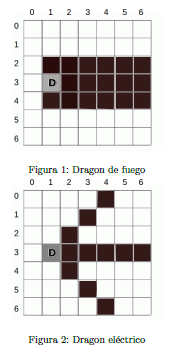
\includegraphics[scale = 1.0]{i1.PNG}\hspace{50mm}  
\end{center} 
\end{figure}
\\Los ataques se hacen en la direcci\'on hacia donde los dragones estan volteando (arriba, abajo, izquierda o
derecha).
\\
Tu trabajo es, dada una cuadricula de $\mathrm{N \times M}$, la cantidad de dragones de fuego y electricos y sus posiciones,
encontrar si existe una casilla que no es alcanzada por los ataques. No se puede estar en la misma casilla en la que
esta un drag\'on.\\
\\
\textrm{\large Entrada}
\\-Un entero $\mathrm{T \leq 100}$, el n\'umero de casos.
\\-Dos enteros $\mathrm{2 \leq N, M \leq 30}$, la dimensi\'on de la cuadr\'icula.
\\-Dos enteros $\mathrm{F}$ y $\mathrm{E}$, la cantidad de dragones de fuego y el\'ectronicos respectivamente.
Despu\'es siguen $\mathrm{F}$ l\'ineas y $\mathrm{E}$ l\'ineas con las siguientes especificaciones: Dos enteros,
$\mathrm{X}$ y $\mathrm{Y}$ y un car\'acter $\mathrm{C}$, donde $\mathrm{X}$ y $\mathrm{Y}$ son las coordenadas 
del drag\'on: Arriba, Abajo, Izquierda y Derecha, representados por los caracteres $\mathrm{U}$, $\mathrm{D}$,
$\mathrm{L}$, $\mathrm{R}$, respectivamente.\\
\\
\textbf{\large Salida}
\\Por cada caso de entrada se debe imprimir "Pelear" si existe una casilla que no es alcanzada por los ataques o
imprimir "Escapar" en el caso contrario.\\
\\
\textbf{\large Entrada Ejemplo}
\\
2\\
9 9\\
3 0\\
0 1 D\\
8 4 u\\
0 7 D\\
3 4\\
1 2\\
0 1 D\\
0 0 R\\
1 0 R\\
\\
\textbf{}{\large Salida Ejemplo}
\\
Escapar\\
Pelear\\
\\
\textbf{}{\large Entendiendo el problema}\\
En este problema te encuentras en una cuadrícula de $n \times m$ ($2 \leq n, m \leq 30$), y se te pide saber si necesitas escapar, o no, después de que ciertas casillas de la cuadrícula sean atacadas por los dragones de la cuadrícula. Siempre que existe al menos una casilla en la cuadrícula que no sea atacada por ningún dragón, no es necesario escapar.\\
\\
\textbf{}{\large Solución}\\
Es posible marcar todas las casillas que ataca cada dragón. Al terminar con todos los dragones se debe recorrer toda la cuadrícula y revisar si existe al menos una casilla no atacada.\\
\\
\textbf{}{\large Código}\\
\begin{minted}[breaklines,fontsize=\footnotesize,linenos]{cpp}
#include <iostream>
#include <cstring>
#define For(i, a, b) for(int i=a; i<b; ++i)
#define FOR(i, a, b) for(int i=a; i>b; --i)
using namespace std;
 
bool mundo[35][35];
int N, M;
 
void fuego(int x, int y, char d)
{
    if (d == 'U')
        FOR(i, y, -1)
        {
            mundo[i][x] = 1;
            if (x-1 >= 0) mundo[i][x-1] = 1;
            if (x+1 < M) mundo[i][x+1] = 1;
        }
    else if (d == 'D')
        For(i, y, N)
        {
            mundo[i][x] = 1;
            if (x-1 >= 0) mundo[i][x-1] = 1;
            if (x+1 < M) mundo[i][x+1] = 1;
        }
    else if (d == 'L')
        FOR(i, x, -1)
        {
            mundo[y][i] = 1;
            if (y-1 >= 0) mundo[y-1][i] = 1;
            if (y+1 < N) mundo[y+1][i] = 1;
        }
    else
        For(i, x, M)
        {
            mundo[y][i] = 1;
            if (y-1 >= 0) mundo[y-1][i] = 1;
            if (y+1 < N) mundo[y+1][i] = 1;
        }
}
 
void electrico(int x, int y, char d)
{
    mundo[y][x] = 1;
    if (d == 'U')
    {
        FOR(i, y-1, -1) mundo[i][x] = 1;
        for(int i=y-1, j=x-1; i >= 0 and j >= 0; i--, j--) mundo[i][j] = 1;
        for(int i=y-1, j=x+1; i >= 0 and j < M; i--, j++) mundo[i][j] = 1;
    }
    if (d == 'D')
    {
        For(i, y+1, N) mundo[i][x] = 1;
        for(int i=y+1, j=x-1; i < N and j >= 0; i++, j--) mundo[i][j] = 1;
        for(int i=y+1, j=x+1; i < N and j < M; i++, j++) mundo[i][j] = 1;
    }
    if (d == 'L')
    {
        FOR(i, x-1, -1) mundo[y][i] = 1;
        for(int i=y-1, j=x-1; i >= 0 and j >= 0; i--, j--) mundo[i][j] = 1;
        for(int i=y+1, j=x-1; i < N and j >= 0; i++, j--) mundo[i][j] = 1;
    }
    if (d == 'R')
    {
        For(i, x+1, M) mundo[y][i] = 1;
        for(int i=y-1, j=x+1; i >= 0 and j < M; i--, j++) mundo[i][j] = 1;
        for(int i=y+1, j=x+1; i < N and j < M; i++, j++) mundo[i][j] = 1;
    }
}
 
int main()
{
    int T;
    cin>>T;
    while(T--)
    {
        int F, E;
        cin>>N>>M>>F>>E;
         
        For(i, 0, N)
            memset(mundo[i], 0, sizeof(mundo[i]));
         
        For(i, 0, F)
        {
            char d;
            int x, y;
            cin>>y>>x>>d;
            fuego(x, y, d);
        }
        For(i, 0, E)
        {
            char d;
            int x, y;
            cin>>y>>x>>d;
            electrico(x, y, d);
        }
        bool escapar = false;
        For(i, 0, N)
            For(j, 0, M)
                if (!mundo[i][j])
                    escapar = true;
                     
        if (!escapar)
            cout<<"Escapar"<<endl;
        else
            cout<<"Pelear"<<endl;
    }
    return 0;
}
\end{minted}

\newpage
\hspace{5 cm}---\textrm{\large E - Escribiendo mensajes\footnote{UVA Online Judge}}\\
\\
\hspace{10 cm}---\textrm{\raggedright\normalsize  Límite de tiempo: 3 segundos}
\\

\hfill
\begin{tabular}{@{}l@{}}
\textbf{Dificultad:} $\star$\\
\textbf{Temas:} Implementación\\
\textbf{Complejidad:} $O(n)$
\end{tabular}\\
\\El flojo fue v\'ictima de un asalto, le robaron su celular y ahora tiene un viejo celular que tiene un teclado como
el siguiente:
\begin{figure}[h!] 
\begin{center} 
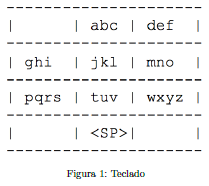
\includegraphics[scale = 1.0]{i2.PNG}\hspace{50mm}  
\end{center} 
\end{figure}
\\Al 
flojo Mau no le gusta ese celular porque para escribir una letra tiene que presionar varias veces una misma
tecla. Por ejemplo, para escribir la "a", \'el tiene que presionar la misma tecla una vez, pero para escribir la "b" tiene
que presionar la misma tecla dos veces, y para la "c", tres veces. Para escribir un espacio, basta con presionar una
vez la tecla $<SP>$.
El fl
ojo Mau tiene que mandar un mensaje de texto con su celular, pero como es muy 
flojo no quiere mandar
el mensaje si debe presionar muchas teclas. Tu tarea es ayudar a contar el n\'umero de teclas que el 
ojo Mau debe
presionar para poder escribir un mensaje.\\
\\
\textrm{\large Entrada}
\\Un entero $\mathrm{T}$, el n\'umero de casos de prueba. Las siguiente $\mathrm{T}$ l\'neas contienen s\'olo espacios y caracteres en
min\'uscula.\\
\\
\textrm{\large Salida}
\\Para cada caso de prueba debes imprimir una l\'inea especificando el n\'umero del caso seguido del n\'umero de
teclas que el 
ojo Mau debe presionar para escribir el mensaje de ese caso.\\
\\
\textbf{}{\large Entrada Ejemplo}\\
2\\
el flojo mau es muy flojo\\
come frutas y verduras\\
\\
\textbf{}{\large Salida Ejemplo}
\\
Case \#1: 52\\
Case \#2: 48\\
\\
\textrm{\large Entendiendo el problema}\\
Dada una cadena de caracteres, se te pide encontrar el número de tecleos necesarios para escribir dicha cadena usando un teclado multitap.\\
\\
\textrm{\large Solución}\\
Lo único que necesitamos es tener el número de tecleos, $T[x]$, necesarios para escribir el caracter $x$. Con esto podemos recorrer la cadena $s$ e ir sumando $T[s[i]]$ a nuestro resultado.\\
\\
\textrm{\large Código}\\
\begin{minted}[breaklines,fontsize=\footnotesize,linenos]{cpp}
#include <iostream>
#include <cstdio>
#define For(i, a, b) for(int i=a; i<b; ++i)
using namespace std;
 
int main()
{
    int T[26];
    for (int i=0, v=0; i<26; i++)
    {
        if (i+'a' == 's' or i+'a' == 'z')
            T[i] = 4;
        else
        {
            T[i] = v+1;
            v = (v+1)%3;
        }
    }
     
    int casos;
    string basura;
    cin>>casos;
    getline(cin, basura);
    For(j, 0, casos)
    {
        int total = 0;
        string L = "";
        getline(cin, L);
        For(i, 0, L.length())
            if (L[i] == ' ') total++;
            else total += T[L[i]-'a'];
        cout<<"Case #"<<j+1<<": "<<total<<endl;
    }
    return 0;
}
\end{minted}

\newpage
\hspace{5 cm}---\textrm{\large F - ¿Y el problema F?\footnote{Mauricio Eduardo Montalvo Guzmán - Grupo de Algorimia Avanzada y Programación Competitiva}}\\
\\
\hspace{10 cm}---\textrm{\raggedright\normalsize  Límite de tiempo: 1 segundo}
\\

\hfill
\begin{tabular}{@{}l@{}}
\textbf{Dificultad:} $\star \star$ \\
\textbf{Temas:} Cadenas, Implementación,\\
Timewaster, Ordenamiento \\
\textbf{Complejidad:} $O(n \log n)$
\end{tabular}\\
\\
\\Se tiene una enorme cadena de caracteres la cual est\'a codificada y tiene ciertas contraseñas escondidas, dependiendo
del tipo y cantidad de contraseñas que contenga la cadena original se le asigna un valor, sabemos que
podemos dividir dicha cadena en $\mathrm{N}$ subcadenas que son propuestas como \'utiles, estas $\mathrm{N}$ subcadenas pueden caer
en uno de los siguientes 4 tipos de cadenas: cadenas pal\'indromos regulares, cadenas espejo, cadenas pal\'indromos
espejo y cadenas basura, cada una de estas cadenas tiene un significado especial y un valor :
\\ 
\begin{enumerate}
\item Pal\'indromos Regulares-Valor 1:
Cadena de caracteres que se lee igual hacia atr'as que hacia adelante. Ejemplo: "RECONOCER".
\item Cadena Espejo - Valor 2:
Cadena de caracteres que, cuando se lee de atr\'as hacia adelante, cada caracter tiene su respectivo "caracter
espejo". Ejemplo: "3SI2E".\\
Aqu\'i se muestra la tabla de caracteres con sus correspondientes espejos, no todos los caracteres tiene un
espejo.
\begin{figure}[h!] 
\begin{center} 
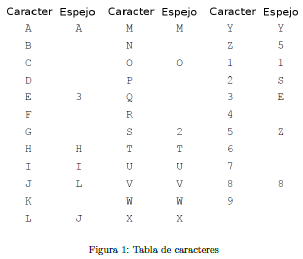
\includegraphics[scale = 1.0]{i3.PNG}\hspace{50mm}  
\end{center} 
\end{figure}
\\
\item Cadena Pal\'indromo Espejo - Valor 3:
Existen caracteres que son su mismo espejo, por ejemplo el espejo de "A" es "A" y el espejo de "8" es "8", una
cadena pal\'indromo espejo es un pal\'indromo compuesto \'unicamente por caracteres que son su mismo espejo.
Ejemplo: "A8OMO8A".
\item Cadena Basura - Valor 0:
Toda cadena que no cumple con alguna de las condiciones anteriores.\\
\end{enumerate}
\'Las cadenas pal\'indromo espejo tengan son las mas especiales debido a que los investigadores estan seguros de que son contraseñas de cuentas bancarias codificadas, sabiendo esto, podemos obtener el valor de la cadena orginal, que es la suma de los valores de sus subcadenas.
Tu tarea es, dado un grupo de $\mathrm{M}$ cadenas obtener cual es la que tiene mayor valor.\\
\\
\textbf{\large Entrada}
\\La primer l\'Inea de entrada sera un n\'umero entero N, que indica el numero de casos de prueba. Cada caso de
prueba comienza con dos enteros $\mathrm{M, (1 \leq M \leq 10)}$ y $\mathrm{P, (1 \leq P \leq 50)}$, que indican el n\'umero de cadenas a evaluar
y el n\'umero de subcadenas que contiene cada cadena, respectivamente. Cada cadena a evaluar esta compuesta por
dos l\'ineas, la primera contiene la cadena y la segunda contiene $\mathrm{P}$ enteros que son los ndices donde termina cada
subcadena, la subcadena 1 comienza en el \'indice 0. La longitud de cada cadena no sobrepasa los 10000 caracteres.\\
\\
\textbf{\large Salida}
\\Para cada caso de prueba debes imprimir una l\'inea especificando el n\'umero del caso seguido del n\'umero de teclas que el ojo Mau debe presionar para escribir el mensaje de ese caso.\\
\\
\textbf{\large Entrada Ejemplo}
\\1\\
2 3\\
NOTAPALINDROMEISAPALINILAPASIMIRRORED\\
13 28 36\\
2A3MEASATOYOTACOSAS\\
6 13 18\\
\\
\textbf{\large Salida Ejemplo}
\\1 5\\
2A3MEAS\\
ATOYOTA\\
\\
\textbf{\large Entendiendo el problema}\\
Se te es dada una serie de cadenas y cada una de ellas está delimitada en subcadenas. Debes decidir cuál cadena es la 
cadena que tiene el mayor puntaje total; donde el puntaje total de 
cada cadena es la suma del puntaje de sus subacadenas, los 
puntajes para cada tipo de subacadena se definen en el problema. Una vez obtenida la cadena con mayor puntaje se deben imprimir, en orden lexicográfico, sus subcadenas que tienen un puntaje mayor a cero.\\
\\
\textbf{\large Solución}\\
El problema anterior es trivial de resolver manteniendo un
vector de vectores con las subcadenas útiles para cada cadena
y al final del procesamiento se obtendría cuál es la que tuvo 
el mayor valor total de manera lineal para después solo ordenar sus
subcadenas útiles, por lo que solo nos quedaría programar 
subrutinas que nos digan si una cadena es palíndroma regular (una cadena $s$ es palíndroma si $s_i = s_{n-i-1}$ $\forall\ i = 0, \dots, n-1$), es espejo (una cadena $s$ es espejo si  $s_i = \text{mirror}(s_{n-i-1}) \ \forall\ i = 0 \dots n-1$, donde, \text{mirror}(c) es una función que regresa el caracter espejo de $c$) o ambas.

Por lo tanto la complejidad del problema sería $O(n m \log n)$ , donde, $n$ es la cantidad de cadenas y $m$ es la longitud de la subcadena más grande de la cadena con el mayor valor.\\
\\
\textbf{\large Código}\\

\begin{minted}[breaklines,fontsize=\footnotesize,linenos]{cpp}
#include <iostream>
#include <algorithm>
#include <vector>
#include <map>
#define For(i, a, b) for(int i=a; i<b; ++i)
using namespace std;

bool isPalindromo(string A)
{
	int m1 = A.length()/2, m2 = A.length()/2;
	if (!(A.length()%2)) m1--;
	
	for(int i = m1, j = m2; i >= 0 and j < A.length(); i--, j++)
		if (A[i] != A[j]) return false;
	return true;
}

bool isEspejo(string A)
{
	char letra[] = {'A', 'E', 'H', 'I', 'J', 'L', 'M', 'O', 'S', 'T', 'U', 'V', 'W', 'X', 'Y', 'Z', '1', '2', '3', '5', '8'};
	char espej[] = {'A', '3', 'H', 'I', 'L', 'J', 'M', 'O', '2', 'T', 'U', 'V', 'W', 'X', 'Y', '5', '1', 'S', 'E', 'Z', '8'};
	map <char, char> letraEsp;
	For(i, 0, 21)
		letraEsp[letra[i]] = espej[i];
		
	int m1 = A.length()/2, m2 = A.length()/2;
	if (!(A.length()%2)) m1--;
	
	for(int i = m1, j = m2; i >= 0 and j < A.length(); i--, j++)
		if (A[j] != letraEsp[A[i]]) return false;
	return true;
}

bool isPalEsp(string A)
{
	char letra[] = {'A', 'H', 'I', 'M', 'O', 'T', 'U', 'V', 'W', 'X', 'Y', '1', '8'};
	bool sirve[26];
	For(i, 0, 13)
		sirve[letra[i]-'A'] = true;
	
	int m1 = A.length()/2, m2 = A.length()/2;
	if (!(A.length()%2)) m1--;
	for(int i = m1, j = m2; i >= 0 and j < A.length(); i--, j++)
		if (A[i] != A[j] or (A[i] == A[j] and !sirve[A[i]-'A'])) return false;
	return true;
}

int main()
{
	int T;
	cin>>T;
	while(T--)
	{
		int M, P, valor[15] = {0}, nEsp[15] = {0};
		vector <vector <string> > utiles;
		string palabra[15];
		cin>>M>>P;
		utiles.assign(M, vector<string> ());
		For(i, 0, M)
		{
			int indice[60];
			cin>>palabra[i];
			For(k, 0, P)
				cin>>indice[k];
			int pos = 0;
			For(k, 0, P)
			{
				string A = "";
				For(j, pos, indice[k]+1)
					A = A + palabra[i][j];
				//cout<<A<<endl;
				pos = indice[k]+1;
				if (isPalEsp(A))
				{
					valor[i] += 3;
					utiles[i].push_back(A);
					nEsp[i]++;
				}
				else if (isEspejo(A))
				{
					valor[i] += 2;
					utiles[i].push_back(A);
				}
				else if (isPalindromo(A))
				{
					valor[i] += 1;
					utiles[i].push_back(A);
				}
			}
		}
		int mayor = 0;
		For(i, 0, M)
			if (valor[i] > valor[mayor])
				mayor = i;
		sort(utiles[mayor].begin(), utiles[mayor].end());
		cout<<palabra[mayor]<<endl;
		cout<<nEsp[mayor]<<" "<<valor[mayor]<<endl;	
		For(j, 0, utiles[mayor].size())
			cout<<utiles[mayor][j]<<endl;	 
	}
	return 0;
}

\end{minted}


\newpage
\subsection{Estructura de datos no lineales}
\hspace{5 cm}---\textrm{\large H - Haciendo Anagramas\footnote{Waterloo Local Contest 2005 September 24 (Richard Krueger)}}\\
\\
\hspace{10 cm}---\textrm{\raggedright\normalsize  Límite de tiempo: 4 segundos}
\\

\hfill
\begin{tabular}{@{}l@{}}
\textbf{Dificultad:} $\star \star$ \\
\textbf{Temas:} Ordenamiento, Cadenas \\
\textbf{Complejidad:} $O(n^2 * m \log m)$
\end{tabular}\\
\\
\\Muchos aficionados a los crucigramas suelen utilizar anagramas (grupos de palabras con las mismas letras en diferente orden) por ejemplo: AMOR, ROMA, OMAR, MORA, RAMO, ARMO y MARO. Sin embargo, no todas las palabras cumplen con este atributo, ya que no importa como trates de ordenar sus letras no podr\'ias formar otra palabra. Estas palabras se llaman ananagramas, un ejemplo es SEXY.
Es obvio que la definici\'on anterior depende del dominio con el que nosotros estemos trabajando, t\'u podr\'ias
pensar que APARCAMIENTO es un ananagrama, pero cualquier m\'edico te podr\'ia desmentir f\'acilmente ya que el te dir\'ia que existe METACARPIANO. Un posible dominio podr\'ia ser todo el idioma español, pero esto podr\'ia acarrear algunos problemas. Nosotros podemos restringir el dominio, por ejemplo, Geograf\'ia, en cuyo caso NEPAL se vuelve un anagrama relativo (PANEL no esta en el mismo dominio), pero QUERETARO no lo es ya que puede transformarse a TERRAQUEO.
T\'u debes escribir un programa que lea un diccionario de un dominio restringido de palabras y determinar todos
los posibles ananagramas relativos. Debes notar que las palabras de una sola letra son, ipso facto, ananagramas
relativos ya que no se pueden "reorganizar"de ning\'un otra forma. Nuestro diccionario no contendr\'ia m\'as de mil palabras.\\
\\
\textbf{\large Entrada}
\\La entrada consiste en una serie de lineas. Ninguna l\'inea tendra mas de 80 caracteres de largo, pero puede
contener cualquier n\'umero de palabras. Las palabras consisten de hasta 20 caracteres (may\'usculas y min\'usculas) letras y no se cortaran entre lineas. Los espacios pueden aparecer libremente entre las palabras y por lo menos un espacio separa m\'ultiples palabras en la misma l\'inea. Tenga en cuenta que las palabras que contienen las mismas letras pero con diferente capitalizaci\'on se consideran anagramas entre si, por ejemplo CoNsErVaDorA y cOnvErsAdOra son anagramas. El archivo de entrada termina con una linea consistente del s\'mbolo \#.\\
\\
\textrm{\large Salida}
\\La salida consistir\'ia de una serie de lineas. Cada l\'inea consistir\'ia de una sola palabra que ser\'ia un ananagrama relativo en el diccionario de entrada. Las palabras deber\'ian ser puestas en orden lexicogr\'afico (sensible a capitalizaci\'on). Se asegura que siempre habr\'a por lo menos unananagrama relativo.\\
\\
\textbf{\large Entrada Ejemplo}
\\ladder came tape soon leader acme RIDE lone Dreis peat\\
ScAlE orb eye Rides dealer NotE derail LaCeS drIed\\
noel dire Disk mace Rob dries\\
\\
\textbf{\large Salida Ejemplo}
\\Disk\\
NotE\\
derail\\
drIed\\
eye\\
ladder\\
soon\\
\\
\\
\textbf{\large Entendiendo el problema}\\
Un ananagrama es una palabra que no es un anagrama, dado un diccionario debemos decir cuáles no son anagramas entre sí.\\
\\
\textbf{\large Solución}\\
Una primera solución ingenua sería ver si cada palabra contra
todas las demás es anagrama relativo y las que no lo son 
marcarlas para después imprimirlas, esto nos dejaría con el 
problema de ver si una palabra es anagrama de otra, esto se 
puede hacer ordenando los caracteres de ambas y si coinciden en
todas sus letras estamos ante dos anagramas, esto nos deja 
ante una solución con complejidad $O(n^2 * m \log m)$ donde 
$n$ es la cantidad de palabras y $m$ es el tamaño de la 
palabra más grande, para este concurso este era la 
complejidad mínima esperada para pasar los casos de prueba 
del juez.

Un segudo enfoque es ordenar cada cadena e insertarlas en un árbol binario de 
búsqueda balanceado; para cada palabra checaremos si es 
que existe dentro de la estructura de datos así evitando la
fuerza bruta cuadrática, esta solución tiene una complejidad de $O(n*m * \log (n) * \log (m))$.\\
\\
\\
\textbf{\large Código}\\

\begin{minted}[breaklines,fontsize=\footnotesize,linenos]{cpp}
#include <bits/stdc++.h>
using namespace std;

set<string> ananagrama;
vector<string> arr;

bool compare(string a, int apos, string b, int bpos)
{
    if(apos != bpos)
    {
        transform(a.begin(), a.end(), a.begin(), ::tolower);
        transform(b.begin(), b.end(), b.begin(), ::tolower);
        sort(a.begin(), a.end());
        sort(b.begin(), b.end());
        if(a == b)
            return true;
        else
            return false;
    }
    return false;
}

int main()
{
    string palabra;
    while((cin >> palabra) and palabra != "#")
    {
        arr.push_back(palabra);
    }
    bool bandera=false;
    for(int i=0; i<(int)arr.size(); ++i)
    {
        bandera = false;
        for(int j=0; j<(int)arr.size(); ++j)
        {
            if ((bandera = compare(arr[i],i, arr[j],j)) and bandera)
                break;
        }
        if( not bandera)
            ananagrama.insert(arr[i]);
    }
    for(set<string>::iterator  i=ananagrama.begin(); i!=ananagrama.end(); ++i)
    {
        cout << *i << "\n";
    }
    return 0;
}

\end{minted}
\newpage
\section{Teor\'ia de N\'umeros}
\newpage
\section{Combinatoria}
%\hspace{1 cm}--- Linus
\hspace{5 cm}---\textrm{\large C - Cortando Pizza\footnote{UVA Online Judge}}\\
\\
\hspace{10 cm}---\textrm{\raggedright\normalsize  Límite de tiempo: 1 segundo}
\\

\hfill
\begin{tabular}{@{}l@{}}
\textbf{Dificultad:} $\star \star$ \\
\textbf{Temas:} Matemáticas\\
\textbf{Complejidad:} $O(1)$
\end{tabular}
\\
\\Ricardo dice ser muy inteligente y que su inteligencia y perspicacia le ayudar\'an en todo. \'El dice que si su
inteligencia le permite hacer una actividad realizando un esfuerzo f\'isico menor ¿Por que debe de cansarse m\'as de
la cuenta? Tambi\'en \'el dice que si usa su cerebro para realizar un menor esfuerzo no es por holgazaner\'ia sino una
muestra elegante de su superioridad intelectual.
En alguna ocasi\'on Ricardo se pregunt\'o c\'omo cortar una pizza en siete rebanadas y repartirlas entre sus amigos,
para ello el tamaño de las rebanadas puede no ser el mismo. Pens\'o un poco y lleg o a la conclusi\'on de que pod  a
obtener las siete rebanadas realizando s\'olo tres cortes -de orilla a orilla- a la pizza, con un cortador de pizza.
Aqu\'i mostramos la forma en que Ricardo cort\'o aquella pizza:
\\
\begin{figure}[h!] 
\begin{center} 
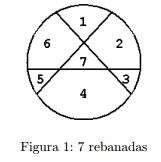
\includegraphics[scale = 1.0]{reb.PNG}\hspace{50mm}  
\end{center} 
\end{figure}
\\
Uno de sus amigos, quien nunca crey\'o en la inteligencia de Ricardo, pens\'o "Si Ricardo puede hacerlo, ¿Por qu\'e no
podr\'ia hacerlo mi computadora?" As\'i que este amigo intento hacer algo similar (pero no exactamente igual a \'el
porque Ricardo lo criticar\'ia por haberle robado la idea) con ayuda de su computadora. \'El escribi\'o un programa que
dado el n\'umero de cortes en la pizza dice el n\'umero m\'aximo de rebanadas que se pueden obtener con exactamente
ese n\'umero de cortes.
Tu trabajo aqu\'i es escribir un programa similar. Es seguro que el amigo de Ricardo no te criticar\'a por hacer el
mismo trabajo que \'el.
\\
\textrm{\large Entrada}
\\
El archivo de entrada contiene un entero por l\'inea "....Ecuación... n (0 <= n <= 4, 295, 113, 503" que representa el n\'umero de
cortes que se deben hacer de lado a lado de la pizza. Un n\'umero negativo con entrada.
\\
\textrm{\large Salida}
\\
La salida debe ser un entero, el n\'umero m\'aximo de rebanadas que se pueden producir.
\\
\textrm{\large Entrada Ejemplo}
\\
5\\
10\\
-100\\
\\
\textrm{\large Entrada Ejemplo}
\\
16\\
56\\
\\
\textrm{\large Entendiendo el problema}\\
\\El problema se puede ver como el máximo número de regiones en las que el plano puede ser cortado con $n$ líneas, el cual es un problema muy conocido.\\ 

\textrm{\large Solución}\\
\\Definamos nuestro resultado como $f(n)$. Claramente $f(1) = 2$, y dado que cada nueva línea nos crea $n$ nuevas secciones, ya que divide cada sección en dos, entonces $f(n) = f(n-1) + n$.
Por lo tanto:
\begin{align*}
f(n) & = n + f(n-1) \\
     & = n + n-1 + f(n-2) \\
     & = n + n-1 + ... + 2 + f(1) \\
     & = n + n-1 + ... + 2 + 1 + 1 \\
     & = \sum_{i = 1}^n i + 1 \\
     & = \frac{n(n+1)}{2} + 1
\end{align*}\\
\textrm{\large Código}\\
\begin{minted}[breaklines,fontsize=\footnotesize,linenos]{cpp}
#include<iostream>
using namespace std;
int main()
{
    long long quesos = 0, n;
    cin >> n;
    while(n >= 0)
    {
        quesos = n*(n+1)/2 + 1;
        cout << quesos << endl;
        cin >> n;
    }
    return 0;
}
\end{minted}

\newpage
\section{Teor\'ia de Gr\'aficas}
\newpage
%\hspace{1 cm}--- Linus
\hspace{5 cm}---\textrm{\large B - Buscando Oro\footnote{LightOJ Online Judge}}\\\\
\\
\hspace{10 cm}---\textrm{\raggedright\normalsize  Límite de tiempo: 3 segundos}
\\

\hfill
\begin{tabular}{@{}l@{}}
\textbf{Dificultad:} $\star \star \star \star$\\
\textbf{Temas:} Grafos, \\Programación dinámica\\
\textbf{Complejidad:} $O(k^2 2^k)$
\end{tabular}\\
\\
\\Has descubierto la Ciudad de Oro. Como te encanta el oro, has empezado a recolectarlo. Pero hay tanto oro
que te est\'as cansando mientras lo recolectas, as\'i que quieres saber cu\'al es el m\'inimo esfuerzo necesario para
obtener todo el oro.
La ciudad est\'a descrita con una cuadr\'icula 2D, donde tu posici\'on inicial est\'a marcada con una 'x'. Un espacio
vac\'io se denotar\'a con un '.'. Y los lugares que contienen oro se denotar\'an con una 'g'. En cada movimiento
puedes desplazarte a todos los 8 lugares adyacentes dentro de la ciudad.\\
\\
\textrm{\large Entrada}
\\
\\La primera l\'inea ser\'a un entero T (1 <= T <= 100), que denota el n\'umero de casos. Cada caso empezar\'a con
dos enteros, m y n (0 < m; n <= 20) denotando los renglones y columnas de la ciudad, respectivamente. Las
siguientes m l\'ineas contienen n caracteres que describen las ciudad. Habr\'a s\'olo una 'x' en la ciudad y a lo m\'as
15 posiciones de oro.\\
\\
\textrm{\large Salida}
\\
\\Para cada caso de prueba debes imprimir un entero indicando el m\'inimo n\'umero de pasos requeridos para
recolectar todo el oro de la ciudad y regresar a la posici\'on inicial.\\
\\
\textrm{\large Entrada Ejemplo}
\\
2\\
5 5\\
x....\\
g....\\
g....\\
.....\\
g....\\
5 5\\
x....\\
g....\\
g....\\
.....\\
.....\\
\\
\textrm{\large Salida Ejemplo}
\\
Case 1: 8\\
Case 2: 4\\
\\

\textrm{\large Entendiendo el problema}\\
\\Dada una cuadrícula de $n \times m$ ($1 \leq n, m \leq 20$), donde existen $k$ ($1 \leq k \leq 15$) posiciones especiales, y una posición inicial, se pide encontrar el mínimo número de pasos necesarios para pasar por todas las $k$ posiciones especiales y regresar a la posición inicial.\\
\\
\textrm{\large Solución}\\
\\Para resolver el problema hay que notar que lo que necesitamos es un ciclo hamiltoniano mínimo. El conjunto de vértices del grafo serán las $k$ posiciones especiales más la posición inicial, y dos vértices $u$, $v$, estarán unidos por una arista con peso igual al número mínimo de pasos para llegar de $u$ a $v$. Debido a que para cada posición de la cuadrícula es posible moverse a los 8 vecinos adyacentes, la distancia mínima entre dos posiciónes es la norma uniforme entre ellas. Una vez construido el grafo hay que encontrar el ciclo hamiltoniano mínimo utilizando programación dinámica.\\
\\
\textrm{\large Código}\\
\begin{minted}[breaklines,fontsize=\footnotesize,linenos]{cpp}
#include <iostream>
#include <cstring>
#include <cstdlib>
#include <cstdio>
#include <vector>
#include <map>
#define For(i, a, b) for(int i=a; i<b; ++i)
using namespace std;
 
struct punto
{
    int x, y;
};
 
struct nodo
{
    string S;
    int pos[20];
};
 
int tabla[30][35000];
nodo I[35000];
int dist[30][30], N = 1;
map <string, int> Ind;
 
int max(int a, int b)
{
    return a > b ? a : b;
}
 
void getSubStrings(int t, int x, int n, int* pos, string A)
{
    A = A + (char)(x+'0');
    if (t == n)
    {
        Ind[A] = *pos;
        I[*pos].S = A;
        For(k, 1, A.length())
        {
            string B = A;
            int u = int(B[k]-'0');
            B.replace(k, 1, "");
            I[*pos].pos[u] = Ind[B];
        }
        (*pos)++;
        return;
    }
 
    for( ; x < N-1; x++)
        getSubStrings(t+1, x+1, n, pos, A);
}
 
void iniTabla()
{
    int pos = 0;
    For(i, 0, N)
        getSubStrings(0, 0, i, &pos, "");
}
 
void HamCycle()
{
    For(i, 0, N)
        tabla[i][0] = dist[i][0];
 
    For(j, 1, 1<<(N-1))
    {
        For(i, 0, N)
        {
            if (j == (1<<(N-1))-1 and i) return;
            int min = -1;
            For(k, 1, I[j].S.length())
            {
                int u = int(I[j].S[k]-'0'), S_u = I[j].pos[u];
                if (tabla[u][S_u] + dist[u][i] < min or min == -1)
                    min = tabla[u][S_u] + dist[u][i];
            }
            tabla[i][j] = min;
        }
    }
}
 
int main()
{
    //freopen("entrada.in","r",stdin);
    punto pos[20];
    string mundo[20];
    int T;
    cin>>T;
    For(casos, 0, T)
    {
        int R, C;
        cin>>R>>C;
        For(i, 0, R)
            cin>>mundo[i];
        For(i, 0, R)
            For(j, 0, C)
                if (mundo[i][j] == 'x')
                {
                    pos[0].x = j;
                    pos[0].y = i;
                }
                else if (mundo[i][j] == 'g')
                {
                    pos[N].x = j;
                    pos[N].y = i;
                    N++;
                }
        For(i, 0, N)
            For(j, i+1, N)
                dist[i][j] = dist[j][i] = max(abs(pos[i].x - pos[j].x), abs(pos[i].y - pos[j].y));
 
        iniTabla();
        HamCycle();
        cout<<"Case "<<casos+1<<": "<<tabla[0][(1<<(N-1))-1]<<endl;
        Ind.clear();
        N = 1;
    }
    return 0;
}
\end{minted}
\newpage
%\hspace{1 cm}--- Linus
\hspace{5 cm}---\textrm{\large G - Guiando a Mau por el Bosque\footnote{Waterloo Local Contest 2005 September 24 (Richard Krueger)}}\\
\\
\hspace{10 cm}---\textrm{\raggedright\normalsize  Límite de tiempo: 3 segundos}
\\

\hfill
\begin{tabular}{@{}l@{}}
\textbf{Dificultad:} $\star \star \star \star$ \\
\textbf{Temas:} Teoría de Grafos, Programación Dinámica \\
\textbf{Complejidad:} $O(E + V \log V)$
\end{tabular}\\
\\
\\El flojo Mau se estresa mucho en su trabajo. Para relajarse despu\'es de un d\'ia dif\'icil a \'el le gusta caminar a casa.
Para hacer las cosas a\'un mejores, su ofcina est\'a en un lado del bosque y su casa del otro. Una caminata tranquila
por el bosque viendo los p\'ajaros y las ardillas es muy agradable. El bosque es hermoso y el fl
ojo Mau quiere tomar
una ruta diferente cada d\'ia. \'El tambi\'en quiere llegar a su casa antes del anochecer, por lo que siempre toma un
camino para avanzar hacia su casa. \'El toma un camino de A a B si existe una ruta desde B a su casa que es m\'as
corta que cualquier ruta posible desde A. Calcula cu\'antas rutas diferentes puede tomar el fl
ojo Mau desde su oficina
a la casa.\\
\\
\textrm{\large Entrada}
\\
\\La entrada contiene varios casos de prueba seguidos por una l\'inea que contiene un 0. El fl
ojo Mau ha numerado
cada intersecci\'on de diferentes caminos, empezando con el 1. Su oficina est\'a numerada con el 1 y su casa con el
2. La primera l\'inea de cada caso contiene el n umero de intersecciones $N (1 < N >= 10^3)$, y el n\'umero de caminos
M. Las siguientes M l\'ineas contienen, cada una, un par de intersecciones y un entero d (1 <= d <= 1000) indicando
que hay un camino de longitud d entre dichas intersecciones. El fl
ojo Mau puede atravezar un camino en cualquier
direcci\'on. Hay a lo m\'as un camino entre cada par de intersecciones.\\
\\
\textrm{\large Salida}
\\
\\Para cada caso de prueba debes imprimir un s\'olo entero m\'odulo 1000000009 indicando el n\'umero de rutas
diferentes que el fl
ojo Mau puede tomar.\\
\\
\textrm{\large Entrada Ejemplo}
\\
5 6\\
1 3 2\\
1 4 2\\
3 4 3\\
1 5 12\\
4 2 34\\
5 2 24\\
7 8\\
1 3 1\\
1 4 1\\
3 7 1\\
7 4 1\\
7 5 1\\
6 7 1\\
5 2 1\\
6 2 1\\
0\\
\\
\textrm{\large Salida Ejemplo}
\\
2\\
4\\
\\
\\
\textrm{\large Entendiendo el problema}\\
Dado un grafo, encontrar la cantidad de rutas distintas que hay entre el origen $s$ y el destino $t$ con la restricción de que sólo se puede ir de un nodo $u$ a un nodo $v$ si la distancia mínima de $v$ a $t$ es menor que la distancia mínima de $u$ a $t$.\\
\\
\textrm{\large Solución}\\
Se puede observar que el grafo generado por sólo seguir dichas aristas 
es un grafo dirigido acíclico (DAG por sus siglas en inglés), que se puede generar fácilmente sacando todas las distancias desde $t$ a todos los demás nodos con un algoritmo Dijkstra en $O(E+V \log V)$ y después con un pase a la lista de adyacencia formamos nuestro DAG.
\\
Sobre un DAG la respuesta al número de caminos posibles desde un origen
es bien conocido y se obtiene vistando los nodos en un orden topológico (DFS o BFS para obtener el orden $O(V+E)$) de manera que cuando visitemos un nodo ya habremos visitado todos los nodos que nos llevan a él usando la siguiente recurrencia:
\[
\displaystyle f(s, u) = \begin{cases} 1 & u = s \\ \sum_{e = (v, u) \in E} \, f(s, v) & \text{cualquier otro caso} \end{cases}
\]
done la línea de abajo nos dice que sumemos todas las aristas que llegan a $u$ desde $v$, es decir, la cantidad de caminos que llegan a un nodo es la suma de la cantidad de caminos que llegan él.

Por último puesto que la respuesta puede ser muy grande usamos aritmética modular para 
presentar la solución.\\
\\
\textrm{\large Código}\\

\begin{minted}[breaklines,fontsize=\footnotesize,linenos]{cpp}
#include <bits/stdc++.h>
using namespace std;
//look at my code my code is amazing
#define FOR(i, a, b) for (int i = int(a); i < int(b); i++)
#define FOREACH(it, a) for (typeof(a.begin()) it = (a).begin(); it != (a).end(); it++)
#define ROF(i, a, b) for (int i = int(a); i >= int(b); i--)
#define REP(i, a) for (int i = 0; i < int(a); i++)
#define INF 1000000000
#define INFLL 1000000000000000000LL
#define ALL(x) x.begin(), x.end()
#define MP(a, b) make_pair((a), (b))
#define X first
#define Y second
#define EPS 1e-9
#define DEBUG(x)   cerr << #x << ": " << x << " "
#define DEBUGLN(x) cerr << #x << ": " << x << " \n"
typedef pair<int, int> ii;
typedef vector<int> vi;
typedef long long ll;
typedef vector<bool> vb;
//ios_base::sync_with_stdio(0);//fast entrada/salida ;-)
//cin.tie(NULL); cout.tie(NULL);
int V, E;
vector< vector<pair<ll,ll> > > AdjList;
vector< vector<ll> > daglist;
vi dist, paths;
vb visited;
vi topo;

void toposort(ll u)
{
	visited[u] = true;
	REP(i, daglist[u].size())
	{
		ll v = daglist[u][i];
		if(not visited[v])
		{
			toposort(v);
		}
	}
	topo.push_back(u);
}

void solve()
{
	AdjList.assign(V, vector<pair<ll,ll> >());
	daglist.assign(V, vector<ll>());
	visited.assign(V, false);
	topo.assign(0, 0);
	REP(i, E)
	{
		ll u, v, w;
		cin >> u >> v >> w;
		u--, v--;
		AdjList[u].push_back(pair<ll,ll> (v, w));
		AdjList[v].push_back(pair<ll,ll> (u, w));
	}
	set<ii> cola;
	dist.assign(V, INF);
	paths.assign(V, 0);
	paths[0] = 1;
	dist[1] = 0;
	cola.insert(ii(0, 1));
	while(not cola.empty())
	{
		ll u = (*(cola.begin())).Y;
		ll d = (*(cola.begin())).X;
		cola.erase(cola.begin());
		if(d > dist[u])
			continue;
		REP(i, AdjList[u].size())
		{
			ll v = AdjList[u][i].X;
			ll w = AdjList[u][i].Y;
			if(d+w <= dist[v])
			{
				dist[v] = d+w;
				cola.insert(ii(dist[v], v));
			}
		}
	}
	REP(u, AdjList.size())
	{
		REP(i, AdjList[u].size())
		{
			int v = AdjList[u][i].X;
			if(u != v and dist[v] < dist[u])
			{
				daglist[u].push_back(v);
			}
		}
	}
	toposort(0);
	ROF(i, topo.size()-1, 0)
	{
		ll u = topo[i];
		REP(j, daglist[u].size())
		{
			ll v = daglist[u][j];
			paths[v] = (paths[v] + paths[u]) % 1000000009LL;
		}
	}
	cout << paths[1] << '\n';
}

int main()
{
	ios_base::sync_with_stdio(0);//fast entrada/salida ;-)
	cin.tie(NULL); cout.tie(NULL);
	while(cin >> V and V)
	{
		cin >> E;
		solve();
	}
	return 0;
}
\end{minted}

\newpage
\section{Paradigmas de programaci\'on}
\subsection{Greedy}
%\hspace{1 cm}--- Linus
\hspace{5 cm}---\textrm{\large A - Abejas\footnote{Mauricio Eduardo Montalvo Guzmán - Grupo de Algorimia Avanzada y Programación Competitiva}}\\
\\
\hspace{10 cm}---\textrm{\raggedright\normalsize  Límite de tiempo: 1 segundo}
\\

\hfill
\begin{tabular}{@{}l@{}}
\textbf{Dificultad:} $\star \star$ \\
\textbf{Temas:} Geometría, Ordenamiento, \\
Algoritmos Voraces \\
\textbf{Complejidad:} $O(n \log n)$
\end{tabular}\\
\\
\\Era un hermoso viernes al medio d\'ia en la FES Acatl\'an, los j\'ovenes estudiantes descansaban tranquilamente en los pastos y las bancas de las \'areas comunes de la FES, cuando de pronto, un cumulo de abejas comenz\'o a atacar a las personas, las abejas sal\'an de todos lados y picaban a cualquier persona que se pusiera en su camino, todos
comenzaron a correr tratando de huir de las abejas pero para algunos estudiantes les fue imposible escapar, extraño
¿no?
Despues de varios d\'ias de investigaci\'on, los integrantes del Grupo de Algoritmia resolvieron el gran misterio
acerca del evento de las abejas, un estudiante de MAC, llamado Peter, fue el culpable del acontecimiento. Peter era
un chico muy extraño y callado, descubrieron que ten\'a un odio irracional hacia las personas y por eso avent\'o un
panal de abejas aquel d\'a.
A pesar de todo, Peter era un chico muy inteligente y no hac\'ia las cosas al azar, descubrieron que, basandose
en sus conocimientos de matem\'aticas y computaci\'on, logro desarrollar un sistema perfectamente elaborado para
molestar a la gente. Peter ve\'ia a la FES como una gran cuadr\'cula (similar al plano cartesiano) donde pod\'ia
identicar la posici\'on de cualquier objeto con sus coordenadas en $\mathrm{X}$ y $\mathrm{Y}$ , as\'i es como logr\'o identificar las posiciones
de todos los panales de abejas que hab\'a en la FES. Ya que tena identificados los panales s\'olo esperaba a que hubiera
una hora pico donde cierto n\'umero N de personas se encontraran cerca de un panal, en ese momento comenzaba
su proceso para molestar. Peter sab\'a que si golpeba el panal con cierta fuerza $\mathrm{F}$ las abejas saldr\'ian muy enojadas
y picar\'ian a todo aquel que se encontrara en un radio $\mathrm{R}$ alrededor del panal, muchas veces era imposible poder
afectar las $\mathrm{N}$ personas cerca del panal as\' que Peter eleg\'a un n\'Uumero $\mathrm{K}$, $\mathrm{(K \leq N)}$, de personas a las que al menos
quer\'a afectar. J\'amas se logr\'o descubrir como es que Peter calculaba el nivel de fuerza $\mathrm{F}$ con el que era necesario
golpear un panal.
La historia de Peter es muy interesante, tan interesante que t\'u est\'as obsesionado con poder emular el proceso
que ten\'a Peter para molestar a la gente, as\'i que desarrollar\'as un programa al que dadas las coordenadas de un
panal, el n\'umero de personas cerca del panal y el n\'umero de personas a las que Peter quer\'ia molestar, calcule el
area m\'inima de la zona afectada por las abejas para poder molestar al menos al n\'umero de personas que Peter
eligi\'o.\\
\\
\\
\textrm{\large Entrada}
\\La primer l\'inea de entrada ser\'ia un entero $\mathrm{C}$, $\mathrm{(1 < C \leq 500)}$ que indica el n\'umero de casos de prueba. Cada caso de prueba comienza con una l\'inea que contiene dos n\'umeros flotantes $\mathrm{PX}$ y $\mathrm{PY}$ , $\mathrm{(-500 \leq PX, PY \leq 500)}$ que indican las coordenadas del panal, la siguiente l\'inea contiene dos enteros $\mathrm{N}$ y $\mathrm{K}$, $\mathrm{(1 < K \leq N < 200)}$ que
indican el n\'umero de personas cerca del panal y el n\'umero de personas que Peter quiere molestar respectivamente, de ah\'i siguen N l\'ineas donde cada una contiene dos n\'umeros flotantes $\mathrm{X_i, Y_i}$, $\mathrm{(-500 \leq X_i; Y_i \leq 500)}$ que indican
las coordenadas de la persona i, cada caso de prueba termina con un \*.\\
\\
\textrm{\large Salida}
\\Por cada caso de entrada se debe imprimir "Pelear" si existe una casilla que no es alcanzada por los ataques o
imprimir "Escapar" en el caso contrario.\\
\\
\textrm{\large Entrada Ejemplo}
\\2\\
9 9\\
3 0\\
0 1 D\\
8 4 u\\
0 7 D\\
3 4\\
1 2\\
0 1 D\\
0 0 R\\
1 0 R\\
\\
\textrm{\large Salida Ejemplo}
\\Escapar\\
Pelear\\
\\


\textrm{\large Entendiendo el problema}
\\Dado un punto base y $n$ puntos adicionales, quieres saber cuál es el área mínima del círculo que cubre al menos $k$ puntos adicionales con centro en el punto base.\\

\textrm{\large Solución}
\\Siguiendo una estrategia \textit{greedy}, o voraz, podemos ver 
que el círculo que buscamos es aquél que tiene como radio la distancia al $k$-ésimo punto más cercano al centro.\\

\textrm{\large Código}
\\La dificultad recae en implementar un algoritmo de ordenamiento cuya complejidad sea $O(n\log n)$ y ordenar por distancias, pero aprovechando las bondades de la \texttt{STL} de \texttt{C++} tenemos lo siguiente.

\begin{minted}[breaklines,fontsize=\footnotesize,linenos]{cpp}
#include <iostream>
#include <cstdio>
#include <algorithm>
#define For(i, a, b) for(int i=a; i<b; ++i)
#define PI 3.14159265359
using namespace std;

struct punto
{
	double x, y, dist;
};

bool myfunction(punto A, punto B){ return A.dist < B.dist; }

int main()
{
	int T;
	cin>>T;
	while (T--)
	{
		double Cx, Cy;
		int N, K;
		string basura;
		punto puntos[200];
		cin>>Cx>>Cy>>N>>K;
		For(i, 0, N)
		{
			cin>>puntos[i].x>>puntos[i].y;
			puntos[i].dist = (Cy-puntos[i].y)*(Cy-puntos[i].y) + (Cx-puntos[i].x)*(Cx-puntos[i].x);
		}
		cin>>basura;
		sort(puntos, puntos+N, myfunction);
		printf("%.2lf\n",PI*puntos[K-1].dist);
	}
	return 0;
}
\end{minted}

\newpage
\newpage
\section{Concurso de programación}{\large XII semana de MAC}\\
\\
%\hspace{1 cm}--- Linus
\hspace{5 cm}---\textrm{\large A - Asombroso League of Legends\footnote{Sergio Adrián Lagunas Pinacho - Grupo de Algorimia Avanzada y Programación Competitiva}}\\
\\
\hspace{10 cm}---\textrm{\raggedright\normalsize  Límite de tiempo: 3 segundos}
\\

\hfill
\begin{tabular}{@{}l@{}}
\textbf{Dificultad:} $\star$ \\
\textbf{Temas:} Ad-hoc \\
\textbf{Complejidad:} $O(1)$
\end{tabular}\\
\\
\\League of Legends es un juego clasificaci\'on MOBA (Multiplayer Online Battle Arena), en el que combaten varios
campeones en enfrentamientos \'epicos, en los que el equipo que juegue mejor en equipo gana.
En \'este problema nos centraremos en 2 campeones, Lux y Volibear; Volibear est\'a persiguiendo a Lux, la cu\'al
tiene poca vida, tal que si Volibear alcanza a Lux, \'esta morir\'a sin poder hacer nada al respecto.
Afort
unadamente, Lux tiene un hechizo que le permite hacer que Volibear deje de moverse durante cierto
tiempo(T); el hechizo lo puede usar cada C segundos (a C tambi\'en se le llama "enfriamiento" de hechizo).
Tu tarea consiste en, sabiendo las velocidades de los campeones (Lux y Volibear), el tiempo que el hechizo de
Lux deja atrapado a Volibear, y el enfriamiento del hechizo de Lux, determinar si Lux ser\'a alcanzada por Volibear
o no.\\
\\
\textrm{\large Entrada}
\\
\\La primera l\'inea contendr\'a un n umero N $(0 < N \leq 100)$, siendo N el n\'umero de casos de prueba. Cada una
de las siguientes N l\'ineas tendr\'a 4 enteros, V1, V2, T y C, $(0 < V1,V2 \leq 500)  (0 < T,C <= 10)$ las velocidades de
Volibear, Lux, el tiempo que el hechizo de Lux atrapa a Volibear, y el enfriamiento de su hechizo respectivamente.
(Las velocidades V1 y V2 est\'an dadas en unidades/segundo, y T,C est\'an dados en segundos. Tambi\'en supon-
dremos que Volibear y Lux empiezan en puntos diferentes, Lux est a adelante de Volibear, y ambos corren en l\'nea
recta)\\
\\
\textrm{\large Salida}
\\
\\Para cada caso de prueba, se tendr\'a que imprimir una l\'inea, imprimiendo "Se muere" si Volibear alcanza a Lux,
y "Se salva" en caso contrario.
\\
\\
\textrm{\large Entrada Ejemplo}
\\
2\\
10 300 1 2\\
300 100 1 10\\
\\
\textrm{\large Salida Ejemplo}
\\
\\Se salva\\
Se muere\\
\\
\textrm{\large Entendiendo el problema}\\
Hay dos objetos que se mueven sobre una recta infinita,
cuya posición al inicio es distinta una del otro, y quieres saber si el objeto $a$ puede alcanzar al objeto $b$ en algún momento en el tiempo; sabiendo que, el objeto $a$ se mueve a una velocidad $v_a$ durante $c$ segundos y se mantiene inmóvil durante $t$ segundos,  mientras que el objeto $b$ nunca para de moverse a una velocidad constans $v_b$.\\
\\
\textrm{\large Solución}\\
Si observamos lo que pasa durante un ciclo de tiempo de tamaño $c+t$ podemos ver que el objeto $a$ (el que persigue) solo se moverá $c * v_a$ unidades de distancia mientras que el objeto $b$ se moverá $(c+t)*v_b$ unidades de distancia, por lo tanto si $c*v_a \leq (c+t)*v_b$ con cada ciclo de tiempo se irá alejando  o manteniendo la misma distancia a $b$ y en caso contrario $b$ será alcanzado,sin importar donde empiecen.\\
\\
\textrm{\large Código}\\

\begin{minted}[breaklines,fontsize=\footnotesize,linenos]{cpp}
#include <iostream>
#include <cstdio>
using namespace std;

int main()
{
//	freopen("DataLoL.out","w",stdout);
//	freopen("DataLoL.in","r",stdin);
	int n,c1,c2,T,C;
	cin>>n;
	while(n--)
	{
		cin>>c1>>c2>>T>>C;
		c2 *= C;
		c1 = (C - T)*c1;
		if(c1 > c2)
		{
			cout<<"Se muere"<<endl;
		}
		else
		{
			cout<<"Se salva"<<endl;
		}
	}
}

\end{minted}
\newpage
%\hspace{1 cm}--- Linus
\hspace{5 cm}---\textrm{\large B - Boby EL Minotauro\footnote[1]{Modificado de un problema original de UVA Online Judge}}\\
\\
\hspace{10 cm}---\textrm{\raggedright\normalsize  Límite de tiempo: 3 segundos}\\

\hfill
\begin{tabular}{@{}l@{}}
\textbf{Dificultad:} $\star$ \\
\textbf{Temas:} Ad-hoc, Cadenas \\
\textbf{Complejidad:} $O(n)$
\end{tabular}\\
\\
\\
Desafortunadamente para el “flojo Mau”, un día se topó con el malvado minotauro devorador de hombres conocido como ... Boby, y cayó directo en su trampa. Boby no es cualquier minotauro, es un minotauro que habla, pero el sólo entiende frases que son palíndromos. Mau se dió cuenta que si le hablaba con palíndromos a Boby, él lo dejaría ir. Afortunadamente Mau tiene consigo un teléfono inteligente con un programa que identifica frases palindrómicas, el cual tú codificaste para él ... ¿o no?.\\
\\
\textrm{\large Entrada}
\\
\\Te serán dadas muchas frases. Cada frase sólo contendrá letras mayúsculas de la ‘A’ hasta la ‘Z’ y los siguientes
caracteres: ‘.’, ‘,’, ‘!’, ‘?’. El final de la entrada será una línea conteniendo la palabra “HECHO”, que no deberá ser procesada. Cada frase tendrá a lo más 200 caracteres.\\
\\
\\
\\
\textrm{\large Salida}
\\
\\Para cada frase imprime una línea con la palabra “NO SERAS COMIDO” si la frase es un palíndromo, o “OH NO!” si no es un palíndromo.
\\
\\
\textrm{\large Entrada Ejemplo}
\\
\\ROMA TIBI SUBITO MOTIBUS IBIT AMOR.\\
ME DEJARIAS IR?\\
ARRIBA LA BIRRA\\
TRAIGAN AL MINOTAURO!\\
HECHO\\
\\
\\
\textrm{\large Salida Ejemplo}
\\
\\NO SERAS COMIDO\\
OH NO!\\
NO SERAS COMIDO\\
OH NO!\\
\\Anotaciones:
Un palíndromo es una frase que se lee igual de atrás hacia adelante y de adelante hacia atrás. Tienes que determinar si son palíndromos o no, ignorando signos de puntuación.\\
\\
\textrm{\large Entendiendo el problema}\\
El problema te pide saber si una cadena es un palíndromo.\\
\\
\textrm{\large Solución}\\
Se dice que una cadena es un palíndromo si para elemento $s_i$ de la cadena $s$ se cumple que $s_i = s_{n-i+1}$ donde $n$ es el tamaño de cadena e $i = 0, 1, \dots, n-1$ . Podemos checar esto eliminando los caracteres especiales y haciendo la comprobación lineal caracter por caracter, aunque con hacer la comprobación para una mitad es suficiente.\\
\\
\textrm{\large Código}\\

\begin{minted}[breaklines,fontsize=\footnotesize,linenos]{cpp}
#include <cstdio>
#include <iostream>
#include <cstdlib>
#include <cmath>
#include <algorithm>
#include <string>
#include <set>
#include <cctype>
#include <vector>
#include <map>
#include <cctype>
using namespace std;
typedef long long ll;

string frase ;

void solve()
{
	int n = frase.size();
	string frase_bonita = "";

	for (int i = 0; i < n; ++i)
	{
		if(not (frase[i] == '.' or frase[i] == ',' or frase[i] == '!' or frase[i] == '?' or frase[i] == ' ' or frase[i] == '\n') )
		{
		//if(isalpha(frase[i]))
			frase_bonita += frase[i];
		}
	}
	n = frase_bonita.size();
	for (int i = 0, j = n-1; i < (n/2)+1; ++i, --j)
	{
		if(frase_bonita[i] != frase_bonita[j])
		{
			//cout << frase_bonita[i] << " " << frase_bonita[j] << '\n';
			printf("OH NO!\n");
			return;
		}
	}
	printf("NO SERAS COMIDO\n");
}

int main()
{
    //int k = 1;
	while(getline(cin, frase) and frase != "HECHO")
	{
		solve();
	}
	return 0;
}
\end{minted}
\newpage
%\hspace{1 cm}--- Linus
\hspace{5 cm}---\textrm{\large C - Coleccionista\footnote[1]{Maximiliano Vera Luna - Grupo de Algoritmia Avanzada y Programación Competitiva}}\\
\\
\hspace{10 cm}---\textrm{\raggedright\normalsize  Límite de tiempo: 3 segundos}\\
\\

\hfill
\begin{tabular}{@{}l@{}}
\textbf{Dificultad:} $\star$ \\
\textbf{Temas:} Implementación \\
\textbf{Complejidad:} $O(n)$
\end{tabular}\\
\\
\\
Hernán es un joven apasionado por los videojuegos, le gustan de todo género, desde shooters, plataformas, carreras y estrategia hasta llegar a los de aventura. Uno de sus juegos favoritos es Pokémon. Pokémon es un juego en el que tu objetivo es conseguir todos los monstruos disponibles(llamados pokémon) y las medallas de todos los gimnasios para así demostrar que has vencido a los mejores.\\
\\Aunque a Hernán le encantan todas las versiones de este juego, desde Rojo y Azul hasta X y Y, él no siempre quiere capturar a todos los pokémon disponibles en algunas versiones, ya sea porque considera que algunos son débiles o pequeños, e incluso feos.\\
\\Debido a esto(y a que no le gusta hacer algo tan fácil), te ha pedido que le ayudes con una sencilla tarea.\\ \\Dados el número total de pokémon disponibles en cada versión y dos listas de pokémon, la primera será la lista de los que ya posee y la segunda la lista de los que no le interesan, determina las siguientes dos cosas:
\begin{itemize}
\item Cuántos y cuáles pokémon le faltan por capturar (solo de los que le interesan).
\item Cuantos y cuales pokémon que posee puede cambiar, ésto es, los pokémon que ya tiene y no le interesan.
\end{itemize}
Los pokémon se identificarán por enteros para facilitar su procesamiento.\\
\\Es sabido que Hernán no posee mas de una especie del mismo pokémon por versión.\\
\\
\textrm{\large Entrada}
\\
\\La entrada consta de varios casos de prueba.
Cada caso consta de 3 líneas, la primera línea ser´a un entero N, $(10 ≤ N ≤ 1000)$ que indica el total de pokémon en la versión del juego.\\
\\La segunda línea contiene un entero A, $(0 ≤ A ≤ N)$ el número de pokémon que Hernán ha capturado en esa versión, seguido por una lista de A enteros que representan a estos pokémon. Todos estos n´umeros están separados por un espacio.\\
\\La tercera línea contiene un entero X, $(0 (≤ X ≤ N)$ el total de pokémon que no le interesan a Hernán, seguido por X enteros que representan a los mismos. Todos estos números están separados por un espacio. Para facilitar su identificación, los pokémon estan representados por números desde $1$ hasta $N$.\\
\\
\textrm{\large Salida}
\\
\\Para cada caso imprime dos líneas:\\
\\La primera línea será un entero $F$ que representará el número de pokémon que le interesa capturar a Hernán y aún no tiene, seguido por $F$ enteros que representan estos pokémon impresos en orden ascendente.\\
\\La segunda constará de un entero $C$ que representará el número de pokémon que Hernán puede cambiar, seguido por $C$ enteros que serán los pokémon cambiables impresos en orden ascendente.\\
\\
\\
\textrm{\large Entrada Ejemplo}
\\
11\\
5 3 5 9 10 11\\
6 2 3 4 5 9 11\\
\\
\\
\textrm{\large Salida Ejemplo}
\\
4 1 6 7 8\\
4 3 5 9 11\\
\\
\textrm{\large Entendiendo el problema}\\
Dadas la cantidad de pokémon existentes, los pokémon que ya capturaste y los pokémon que no te interesan tener, debes obtener dos cosas:
\begin{itemize}
\item Cuántos y cuáles pokémon que sí te interesan te faltan obtener.
\item Cuántos y cuáles pokémon de los que ya tienes no te interesan.
\end{itemize}
\textrm{\large Solución}\\
Para la solución necesitamos poder almacenar cuáles pokémon tenemos, y de esos cuáles no me interesan. Dado que el número total de pokémon es pequeño ($\leq 1000$), es posible crear arreglos de booleanos, \texttt{yatengo[]} y \texttt{nomeinteresan[]} para este propósito. Para responder la primer pregunta necesitamos contar los pokémon $x$ tales que \texttt{yatengo[x] == false} y \texttt{nomeinteresan[x] == false}. Para la segunda, tenemos que contar aquellos pokémon tales que \texttt{yatengo[x] == true} y \texttt{nomeinteresan[x] == true}.\\
\\
\textrm{\large Código}

\begin{minted}[breaklines,fontsize=\footnotesize,linenos]{cpp}
#include<iostream>
#include<vector>
#include<cstdio>
using namespace std;
int main()
{
    int estampas,aux,tengo,desinteres,cont1,cont2,cont=0;;
    vector<int> yatengo;
    vector<int> nomeinteresan;
    while(cin>>estampas)
    {
        cont1=0;
        cont2=0;
        cont++;
        yatengo.assign(estampas+1,0);
        nomeinteresan.assign(estampas+1,0);
        cin>>tengo;
        for(int i=0;i<tengo;i++)
        {
            cin>>aux;
            yatengo[aux]=1;
        }
        cin>>desinteres;
        for(int i=0;i<desinteres;i++)
        {
            cin>>aux;
            nomeinteresan[aux]=1;
        }
        for(int i=1;i<estampas+1;i++)
        {
            if(nomeinteresan[i]==0 && yatengo[i]==0)
            {
                cont1++;
            }
        }
        cout<<cont1;
        for(int i=1;i<estampas+1;i++)
        {
            if(nomeinteresan[i]==0 && yatengo[i]==0)
            {
                cout<<" "<<i;
            }
        }
        cout<<endl;
        for(int i=1;i<estampas+1;i++)
        {
            if(nomeinteresan[i]==1 && yatengo[i]==1)
            {
                cont2++;
            }
        }
        cout<<cont2;
        for(int i=1;i<estampas+1;i++)
        {
            if(nomeinteresan[i]==1 && yatengo[i]==1)
            {
                cout<<" "<<i;
            }
        }
        cout<<endl;
    }
    return 0;
}
\end{minted}
\newpage
%\hspace{1 cm}--- Linus
\hspace{5 cm}---\textrm{\large D - Dominó\footnote[1]{Maximiliano Vera Luna - Grupo de Algoritmia Avanzada y Programación Competitiva}}\\
\\
\hspace{10 cm}---\textrm{\raggedright\normalsize  Límite de tiempo: 1 segundo}\\
\\

\hfill
\begin{tabular}{@{}l@{}}
\textbf{Dificultad:} $\star\star$ \\
\textbf{Temas:} Búsquedas \\
\textbf{Complejidad:} $O(n \log n)$
\end{tabular}\\
\\
\\Mauricio tiene $N$ piezas de domino en fila. Cada pieza se divide en dos partes iguales en tamaño, - la superior y la inferior -. Cada una de las partes contiene un número del 1 al 6.
\\A Mauricio le encantan los números pares, así que quiere que la suma de los números de las mitades superiores y la suma de los números de las mitades inferiores sea par.\\
\\Para lograr eso, Mauricio puede rotar las piezas de dominó 180 grados. Después de una rotación las mitades cambian de lugares. Esta acción toma 1 segundo. Ayuda a Mauricio a averiguar el tiempo mínimo que debe gastar girando piezas de dominó para que se cumpla lo que él quiere.\\
\\
\textrm{\large Entrada}
\\
\\La primera línea contiene un entero $T(1 < T < 50)$, el número de casos de prueba. Para cada uno de los siguientes $T$ casos, hay una línea que contiene un entero $N(1 ≤ N ≤ 100)$, el número de piezas de dominó que tiene Mau. Las siguientes $N$ líneas contienen dos enteros $X_i, Y_i,(1 ≤ X_i, Y_i ≤ 6)$ cada una, separados por un espacio. \\El número $X_i$ es el que esta escrito inicialmente en la mitad superior del i-ésimo dominó, mientras que $Y_i$ es el que está escrito en la mitad inferior.\\
\\
\textrm{\large Entrada}
\\
\\Para cada caso imprime sólo una línea, esta deberá decir “Caso T: ” seguido por el mínimo de segundos requeridos para realizar la tarea. T es el caso actual empezando a numerarlos desde 1. Si resulta imposible lograr tal tarea, imprime un ’-1’ (sin comillas).\\
\\
\\
\textrm{\large Entrada Ejemplo}
\\
2\\
2\\
4 2\\
6 4\\
1\\
2 3\\
\\
\textrm{\large Salida Ejemplo}
\\
Caso 1: 0\\
Caso 2: -1\\
\\
\textrm{\large Entendiendo el problema}\\
Dado una línea alineada de dominos, debemos verificar si es posible hacer que la suma de las partes inferiores y la suma de las superiores es par, ésto mediante la rotación de las fichas de dominó.\\
\\
\textrm{\large Solución}
Obtenemos las sumas de ambas partes, podemos dividir estas sumas en tres casos:
\begin{enumerate}
\item Si las sumas son pares, el problema esta resuelto y la respuesta es 0.
\item Si una suma es par y la otra impar no existe una solución debido a que cada ficha puede ser o con ambas partes pares o ambas impares o una par y la otra impar, pero al rotar cualquiera de estos tres tipos de fichas se sigue sin obtener una solución.
\item Si ambos sumas son impares, basta con encontrar una ficha con una parte par y la otra impar, al rotarla se obtendra una solución, si tal ficha no existe entonces no hay solución.
\end{enumerate}
\textrm{\large Código}\\

\begin{minted}[breaklines,fontsize=\footnotesize,linenos]{cpp}
#include <iostream>
#include <sstream>
#include <algorithm>
#include <vector>
#include <map>
#include <set>
#include <queue>
#include <list>
#include <stack>
#include <cmath>
#include <cstdlib>
#include <cstdio>
#include <cstring>
#include <cctype>
#include <climits>
using namespace std;
int izq[105],der[105];
int n,sumi,sumd;
 
int main()
{
    int t,cont=0;
    cin>>t;
    while(t--)
    {
        cont++;
        cin>>n;
        cout<<"Caso "<<cont<<": ";
        sumi = sumd = 0;
        bool b = false;
        for(int i=0;i<n;i++)
        {
            cin>>izq[i]>>der[i];
            sumi += izq[i];
            sumd += der[i];
        }
        if((sumi&1) and (sumd&1))
        {
            for(int i=0; i<n; i++)
            {
                if( (izq[i]&1) != (der[i]&1))
                {
                    b = true;
                    break;
                }
            }
            if(b)
                cout<<1<<endl;
            else
                cout<<-1<<endl;
        }
        else if( !(sumi&1) and !(sumd&1) )
        {
            cout<<0<<endl;
        }
        else
        {
            cout<<-1<<endl;
        }
    }
    return 0;
}
\end{minted}
\newpage
%\hspace{1 cm}--- Linus
\hspace{5 cm}---\textrm{\large E- Esto es fácil\footnote[1]{Sergio Adrián Lagunas Pinacho - Grupo de Algoritmia Avanzada y Programación Competitiva}}\\
\\
\hspace{10 cm}---\textrm{\raggedright\normalsize  Límite de tiempo: 5 segundos}\\
\\

\hfill
\begin{tabular}{@{}l@{}}
\textbf{Dificultad:} $\star\star$ \\
\textbf{Temas:} Búsquedas \\
\textbf{Complejidad:} $O(n \log n)$
\end{tabular}\\
\\
\\
Este problema es fácil, tienes que buscar 2 enteros en una lista, tal que sumados den otro número.\\
\\
\textrm{\large Entrada}
\\
\\La primera línea tendrá un número $T$ que representa el número de casos de prueba.\\
\\Las siguientes $3T$ líneas contendrán los casos de prueba, cada caso de prueba tendrá $3$ líneas, la primera línea tendrá un número $N (2 ≤ N ≤ 10000)$ que representa la cantidad de números que tendrá el arreglo, la segunda línea tendrá $N$ números enteros $K_i (1 ≤ i ≤ N) (0 ≤ |K_i| ≤ 10000)$ los números sobre los cuáles tienes que buscar la pareja de números, y la tercera línea tendrá un número entero $M (0 ≤ |M| ≤ 20000)$.\\
\\
\\
\\
\textrm{\large Salida}
\\
\\Se imprimirán $T$ líneas, una por cada caso de prueba, con la palabra “SI” si es que existen 2 números $K_i$ y $K_j$ tales que $K_i + K_j = M$, y “NO” en caso contrario.
\\
\\
\textrm{\large Entrada Ejemplo}
\\
2\\
3\\
1 2 3\\
4\\
5\\
6 7 8 9 10\\
11\\
\\
\textrm{\large Salida Ejemplo}
\\
SI\\
NO\\
\\
\textrm{\large Entendiendo el problema}\\
Dada una lista con $n$ elementos, debemos determinar si existe un par de elementos de la lista cuya suma sea igual a un número $M$ dado.\\
\\
\textrm{\large Solución}\\
Para cada elemento $a_j$ del arreglo A, mientras no hayamos determinado que existe una solucion, debemos verficar si existe $a_k$ tal que $a_j + a_k =M$, eso lo realizamos mediante una busqueda binaria (debemos ordenar los elementos de A); esto debido a la limitante de tiempo del problema, si para cada elemento $a_j \in A$ buscaramos linealmente a su complemento $a_k$, la complejidad sería cuadrada y obtendríamos como veredicto $Tiempo$ $Limite$ $Excedido$.

Nota: Dado que los elementos de $A$ son relativamente pequeños es posible disminuir la complejidad del problema a $O(n)$, esto marcado en un arreglo en la posición $a_i$ si $a_i \in A$, ahorrandonos la el ordenamiento y la busqueda binaria.\\
\\
\textrm{\large Código}

\begin{minted}[breaklines,fontsize=\footnotesize,linenos]{cpp}
#include <iostream>
#include <cstdio>
#include <cstdlib>
#include <algorithm>
#define For(X,A,B) for(X=A; X<B; X++)
#define Maxt 1000
using namespace std;
 
int arr[1000]={0};
int var;
 
void busca(int a,int b,int valor)
{
    if(a == b && arr[b]==valor)
        {var = 1; return;}
    else if(a == b && arr[b]!=valor)
        {var = 0; return;}
 
    int mitad = (a+b)>>1;
 
    if(valor <= arr[mitad])
        busca(a,mitad,valor);
    else
        busca(mitad+1,b,valor);
}
 
int main(int argc, char const *argv[])
{
    //freopen("Data.in","r",stdin);
    //freopen("Data.out","w",stdout);
    int i,j,n,casos,sum,tam,x;
 
    scanf("%d",&casos);
    while(casos--)
    {
        scanf("%d",&tam);
 
        for(i=0; i<tam; i++)
            scanf("%d",&arr[i]);
 
        scanf("%d",&sum);
 
        //Cosas
        var = 0;
        sort(arr,arr+tam);
        For(j,0,tam)
        {
            x = sum - arr[j];
            if(x>0)
                busca(0,tam-1,x);
 
            if(var)
            {
                printf("SI\n");
                break;
            }
        }
        if(var == 0)
            printf("NO\n");
    }
    return 0;
}
\end{minted}
\newpage
%\hspace{1 cm}--- Linus
\hspace{5 cm}---\textrm{\large F- Falsa Simulación\footnote[1]{Sphere Online Judge}}\\
\\
\hspace{10 cm}---\textrm{\raggedright\normalsize  Límite de tiempo: 1 segundo}\\
\\

\hfill
\begin{tabular}{@{}l@{}}
\textbf{Dificultad:} $\star \star$ \\
\textbf{Temas:} Ad-Hoc, Estructuras de Datos\\
\textbf{Complejidad:} $O(n+m)$ construcción,\\ $O(1)$ por consulta.\\
\end{tabular}\\
\\
\\El siguiente problema consta de una simulación muy concreta... ¿o no?. Tendrán una matriz $M$ de tamaño 1234(filas) × 5678(columnas). Está inicialmente llena con enteros desde el 1, 2, . . . , 1234×5678 en orden ascendente de izquierda a derecha y de arriba a abajo. (La primera fila está llena con los enteros 1, 2, . . . , 5678; la segunda
con los enteros 5679, 5680, . . . , 11376, etc) Existen 4 tipos de comandos:\\
\begin{itemize}
\item “R x y” intercambia la $x$-ésima y $y$-ésima fila de $M$.
\item “C x y” intercambia la $x$-ésima y $y$-ésima columna de $M$.
\item “Q x y” imprime $M(x, y)$ (El entero que está en la posición $(x,y)$ en la matriz $M$).
\item “W z” imprime $x$ e $y$ donde $z = M(x, y)$.
\end{itemize}

Entrada\\
\\Te será dada una lista de comandos válidos, uno por línea. La entrada termina con el fin de archivo.\\
\\
\textrm{\large Salida}
\\
\\Cada que recibas el comando “Q x y” imprime una línea con el valor $M(x, y)$, y cada que recibas el comando “W z” imprime una línea con los valores $x$ e $y$ separados por un espacio, la posición en la que se encuentra el número $z$.
\\
\\
\textrm{\large Entrada Ejemplo}
\\
R 1 2\\
Q 1 1\\
Q 2 1\\
W 1\\
W 5679\\
C 1 2\\
Q 1 1\\
Q 2 1\\
W 1\\
W 5679\\
7\\
\\
\textrm{\large Salida Ejemplo}
\\
5679\\
1\\
2 1\\
1 1\\
5680\\
2\\
2 2\\
1 2\\
\\
\textrm{\large Entendiendo el problema}\\
Para el propósito de entender el problema supongamos que se tiene una matriz de $n$ filas por $m$ columnas de la siguiente manera, suponiendo que $n = m = 5$:\\
\begin{figure}[h!] 
\begin{center} 
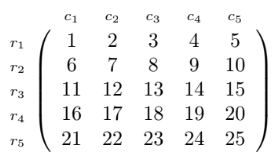
\includegraphics[scale = .8]{a1.PNG}\hspace{50mm}  
\end{center} 
\end{figure}
\\Si quisieramos efectuar la operación \texttt{R 1 2} obtendriamos lo siguiente:
\begin{figure}[h!] 
\begin{center} 
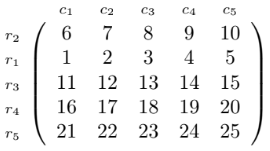
\includegraphics[scale = .8]{a2.PNG}\hspace{50mm}  
\end{center} 
\end{figure}\\
\\ de donde la respuesta para \texttt{W 9} sería \texttt{1 4}.
\\
\\
\textrm{\large Solución}\\

La solución ingenua consiste en mantener una matriz e ir simulando cada uno de las consultas en $O(n)$ u $O(m)$ , pero se puede ver en primera instancia que esta solución no es factible para nuestras restricciones ya que ni siquiera pasaría las restricciones de memoria.

Una solución que nos permite hacer consultas y modificaciones a la matriz en $O(1)$, se logra mediante el uso de dos vectores por renglones y columna uno que te relacione el índice original y índice actual, y visceversa.

\DeclarePairedDelimiter\ceil{\lceil}{\rceil}
\DeclarePairedDelimiter\floor{\lfloor}{\rfloor}
Sólo queda saber que para obtener los índices de una matriz de la forma original dado el valor de $z$ debemos hacer: $x=\floor{z/m}+1$, $y=(z \mod m)+1$; y para obtener $z$ conociendo $x$ y $y$ hacemos: $z=(x-1)m + y$.\\ \\
\\
\textrm{\large Código}

\begin{minted}[breaklines,fontsize=\footnotesize,linenos]{cpp}
#include <iostream>
#include <cstdio>
#include <algorithm>
#include <vector>
using namespace std;
typedef vector<int> vi;

#define N 1234
#define M 5678

vi rows(N+3, 0);
vi cols(M+3, 0);
vi rr = rows;
vi cc = cols;

void solveR()
{
	int x, y;
	scanf("%d %d", &x, &y);
	swap( rows[x], rows[y] );
	rr[rows[x]] = x;
	rr[rows[y]] = y;
}

void solveC()
{
	int x, y;
	scanf("%d %d", &x, &y);
	swap( cols[x], cols[y] );
	cc[cols[x]] = x;
	cc[cols[y]] = y;
}

void solveQ()
{
	int x, y;
	scanf("%d %d", &x, &y);
	printf("%d\n", ((rows[x]-1) * M) + cols[y] );
}

void solveW()
{
	int z;
	cin >> z;
	--z;
	printf("%d %d\n", rr[(z / M)+1], cc[(z%M)+1]);
}

int main()
{
	for (int i = 0; i < M+3; ++i)
	{
		cc[i] = cols[i] = i;
	}
	for (int i = 0; i < N+3; ++i)
	{
		rr[i] = rows[i] = i;
	}
	char orden;
	while(cin >> orden)
	{
		switch(orden)
		{
			case 'R':
				solveR();
				break;
			case 'C':
				solveC();
				break;
			case 'Q':
				solveQ();
				break;
			case 'W':
				solveW();
				break;
		}
	}
	return 0;
}
\end{minted}
\newpage
%\hspace{1 cm}--- Linus
\hspace{5 cm}---\textrm{\large G- Geométra Hermann\footnote[1]{Edgar García Rodríguez - Grupo de Algoritmia Avanzada y Programación Competitiva}}\\
\\
\hspace{10 cm}---\textrm{\raggedright\normalsize  Límite de tiempo: 3 segundos}\\
\\

\hfill
\begin{tabular}{@{}l@{}}
\textbf{Dificultad:} $\star$ \\
\textbf{Temas:} Matemáticas \\
\textbf{Complejidad:} $O(1)$
\end{tabular}\\
\\
\\
Durante el siglo XIX el matemático Hermann Minkowski investigó acerca de un tipo de geometría no euclidiana, llamada geometría de taxi. En la geometría de taxi la distacia entre dos puntos $T_1(x_1, y_1)$ y $T_2(x_2, y_2)$ es definida
como $D(T_1, T_2) = |x_1 − x_2| + |y_1 − y_2|$. \\Cualquier otra definición se define igual que en la geometría euclidiana, incluyendo la definición del círculo: Un círculo es el conjunto de todos los puntos en un plano a una distancia dada(radio) de un punto dado(centro del círculo). \\ \\Nosotros estamos interesados en la diferencia de las áreas de dos
círculos con radio $R$, uno de los cúales está dado en un espacio normal(euclideano) y el otro en una geometría de taxi.\\ Dicha tarea ha sido encomendada a tí.\\
\\
\textrm{\large Entrada}
\\
Cada línea tendrá un solo número entero $1 ≤ R ≤ 10000$. Deberás leer hasta el final del archivo.\\
\\
\textrm{\large Salida}
\\
Para cada caso deberás imprimir dos líneas, la primera contendrá el area del círculo con radio $R$ en una geometría euclidiana y la segunda línea será el area del círculo con radio $R$ en una geometría de taxi. \\ 
\\Tu salida deberá ser redondeada a 4 lugares decimales.\\ 
\\Además puedes asumir de manera segura de usando valores flotantes de precisión doble y $\pi$ igual $3.141592653589793$ será suficiente.
\\
\\
\textrm{\large Entrada Ejemplo}
\\
21\\
9384\\
887\\
\\
\\
\textrm{\large Salida Ejemplo}
\\
1385.4424\\
882.0000\\
276646940.0487\\
176118912.0000\\
2471707.7105\\
1573538.0000\\
\\
\textrm{\large Entendiendo el problema}\\
Debes encontrar el área de un círuclo con radio $r$ utilizando una distancia euclideana y un círculo con radio $r$ utilizando una distancia Manhattan.\\
\\
\textrm{\large Solución}\\
El círculo en una geometría con la distancia euclideana es trivial. Para el otro caso hay que observar que un círculo en una geometría con la distancia Manhattan es en realidad un cuadrado rotado de lado $\sqrt{2r^2}$, por lo tanto su área es $2r^2$.\\
\\
\textrm{\large Código}\\

\begin{minted}[breaklines,fontsize=\footnotesize,linenos]{cpp}
#include <stdio.h>
#include <math.h>
 
int main()
{
    double PI = atan(1.0)*4.0;
    double R;
    while(scanf("%lf", &R)==1)
    {
        printf("%.4lf\n", (double)PI*R*R);
        printf("%.4lf\n", (double)R*R*2.0);
    }
    return 0;
}
\end{minted}
\newpage
%\hspace{1 cm}--- Linus
\hspace{5 cm}---\textrm{\large I- Investigando Laberinto\footnote[1]{Maximiliano Vera Luna - Grupo de Algoritmia Avanzada y Programación Competitiva}}\\
\\
\hspace{10 cm}---\textrm{\raggedright\normalsize  Límite de tiempo: 3 segundos}\\
\\

\hfill
\begin{tabular}{@{}l@{}}
\textbf{Dificultad:} $\star \star$ \\
\textbf{Temas:} Flood fill \\
\textbf{Complejidad:} $O(nm)$
\end{tabular}\\
\\
\\Un laberinto es representado en una cuadrídula de dos dimensiones como está ilustrado en la figura siguiente.
\begin{figure}[h!] 
\begin{center} 
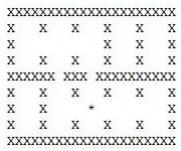
\includegraphics[scale = 1.0]{as.PNG}\hspace{50mm}  
\end{center} 
\end{figure}
Cada punto de la cuadrícula es representado por un carácter. Un carácter espacio ( ) representa los lugares en donde puedes caminar.\\
\\Las paredes del laberinto son representadas por letras mayúsculas (de A a Z), esto es, lugares dónde no puedes caminar.\\
\\Tu tarea es, dado un punto de inicio dentro del laberinto, representado por un asterisco (*), debes de marcar todos los posibles lugares a donde puedes llegar caminando con el carácter gato (\#). El asterisco debe ser reemplazado por el car´acter gato.\\
\\La forma en que puedes caminar es 4 conexidad, esto significa que solo puedes moverte hacia arriba, abajo, izquierda o derecha.\\
\\La cuadricula presentada anteriormente quedaría:
\begin{figure}[h!] 
\begin{center} 
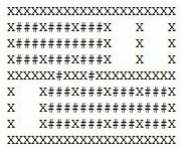
\includegraphics[scale = 1.0]{ad.PNG}\hspace{50mm}  
\end{center} 
\end{figure}
\\
\\
\textrm{\large Entrada}
\\
La primera línea de entrada es $T$, el número de casos. La primera línea de cada caso son dos enteros, $N$ y $M$, el número de renglones y el número de columnas de la cuadrícula respectivamente.\\
\\Las siguientes $N$ lineas contienen $M$ carácteres, las cuales representan al laberinto.\\
\\
\textrm{\large Salida}
\\
$N$ líneas de $M$ carácteres cada una, las cuales representa a la cuadrícula marcada en la forma en que se indicó.\\
\\Imprime una línea en blanco al final de cada caso.\\
\\
\\
\textrm{\large Entrada Ejemplo}
\\
2\\
5 5\\
XXXXX\\
X* X\\
X X\\
XX XX\\
XXXXX\\
5 9\\
AAAAAAAAA\\
C* D B\\
C D B\\
C D B\\
EEEEEEEEE\\
\\
\\
\textrm{\large Salida Ejemplo}
\\
XXXXX\\
X\#\#\#X\\
X\#\#\#X\\
XX\#XX\\
XXXXX\\
AAAAAAAAA\\
C\#\#\#D B\\
C\#\#\#D B\\
C\#\#\#D B\\
EEEEEEEEE\\
\\
\textrm{\large Entendiendo el problema}\\
Dado una cuadrícula de $n \times m$, con algunas paredes dentro de ella, y un punto inicial, se te pide marcar todos los lugares dentro de la cuadrícula a los que puedes llegar, sabiendo que no puedes atravezar paredes y que sólo te puedes mover hacia arriba, abajo, izquierda o derecha.\\
\\
\textrm{\large Solución}\\
Este es un problema muy común y su solución es conocida como algoritmo de relleno por difusión (flood fill en inglés), que es básicamente una búsqueda. 
\\
\textrm{\large Código}\\

\begin{minted}[breaklines,fontsize=\footnotesize,linenos]{cpp}
#include<iostream>
#include<string>
#include<vector>
#include<cstdio>
using namespace std;
vector<string> v;
int dfs(int i,int j)
{
    if(i>0 && j>0 && j<v[i].size() && i <v.size() && v[i][j]!='#' && (v[i][j]==' ' || v[i][j]=='*'))
    {
        v[i][j]='#';
        dfs(i,j+1);
        dfs(i+1,j);
        dfs(i-1,j);
        dfs(i,j-1);
    }
    return 0;
}
int main()
{
    string aux;
    int t,a,b;
    cin>>t;
    while(t--)
    {
        cin>>a>>b;//a=filas, b=columnas
        getline(cin,aux);
        for(int i=0;i<a;i++)
        {
            getline(cin,aux);
            v.push_back(aux);
        }
        for(int k=0;k<v.size();k++)
        {
            for(int l=0;l<v[k].size();l++)
            {
                if(v[k][l]=='*')
                {
                    dfs(k,l);
                }
            }
        }
        for(int k=0;k<v.size();k++)
        {
            cout<<v[k]<<endl;
        }
        cout<<endl;
        v.clear();
    }
    return 0;
}
\end{minted}
\newpage
\hspace{5 cm}---\textrm{\large H- Historia de los Relojes\footnote[1]{Sergio Adrián Lagunas Pinacho - Grupo de Algoritmia Avanzada y Programación Competitiva}}\\
\\
\hspace{10 cm}---\textrm{\raggedright\normalsize  Límite de tiempo: 3 segundos}\\
\\

\hfill
\begin{tabular}{@{}l@{}}
\textbf{Dificultad:} $\star$ \\
\textbf{Temas:} Matemáticas \\
\textbf{Complejidad:} $O(1)$
\end{tabular}\\
\\
\\El interés medieval en contribuciones mecánicas es bien ilustrado por la invención del reloj mecánico, el más viejo el cual es controlado por contrapesos, y un brazo oscilante con un engranage. Esto fué en 1386.\\
\\Los relojes controlador por resortes aparecieron por la mitad del siglo 15, haciendo posible construir mecanismos más compactos, y preparando el camino para el reloj portatil.\\
Los primeros relojes de péndulo controlador por resortes fueron comúnmente puestos en pequeñas repisas de pared, y después sobre repisas. \\Muchos relojes de soporte tenían un cajoncito para guardar la llave del vidrio. Los relojes
de soporte más recientes, hechos después de 1660, tenían diseño arquitectónico, con pilares a los lados.\\
\\El los siglos 17 - 18 en Francia, los relojes de mesa se convirtieron en un objeto de diseño monumental.\\
\\Uno de los primeros relojes atómicos fué un reloj controlado por amoniaco . Este fué hecho en 1949 en el ”National Bureau of Standards”, Washington, D.C.\\
\\La historia de los relojes es fascinante, pero no tiene que ver con éste problema. En éste problema te darán el ángulo entre las manecillas de un reloj en forma de círculo, como el que se muestra en la figura, y tienes que indicar si existe una hora del día tal que el ángulo entre ambas manecillas sea el ingresado por el usuario.\\
\\Para éste problema, supondremos que el reloj tiene 60 marcas, una para cada minuto, y que tanto la manecilla de los minutos, tanto como la de las horas sólo pueden estar apuntando a alguna de las marcas.
\begin{figure}[h!] 
\begin{center} 

\includegraphics[scale = 0.80]{re.PNG}\hspace{50mm}  
\end{center} 
\end{figure}
\\
\\
\\
\textrm{\large Entrada}
\\
Está dada por varias líneas, cada una describiendo un caso de entrada. Cada linea contiene un entero A que
representa el ángulo entre las manecillas $(0 ≤ A ≤ 180)$.
\\
\\
\textrm{\large Salida}
\\
Para cada caso de entrada imprime una línea con la palabra “Caso i: ” (i es el número de caso), seguido por un espacio, seguido por un caracter. Si existe al menos una hora del día tal que el ángulo mínimo entre las manecillas del reloj sea exactamente A grados, imprime el caracter será ”Y”. En caso contrario será ”N”.
\\
\\
\textrm{\large Entrada Ejemplo}
\\
90\\
65\\
66\\
67\\
128\\
0\\
180\\
\\
\\
\textrm{\large Salida Ejemplo}
\\
Caso 1: Y\\
Caso 2: N\\
Caso 3: Y\\
Caso 4: N\\
Caso 5: N\\
Caso 6: Y\\
Caso 7: Y\\
\\
\textrm{\large Entendiendo el problema}\\
Dado un ángulo, quieres saber si es posible que las dos manecillas de un reloj convencional, con 60 marcas, pueden crear dicho ángulo.\\
\\
\textrm{\large Solución}\\
Dado que sólo hay 60 marcas en el reloj, los 360 grados estarán divididos en 60 marcas separadas por 6 grados, así que las manecillas podrán formar un ángulo si y sólo si el ángulo es múltiplo de 6.\\
\\
\textrm{\large Código}\\

\begin{minted}[breaklines,fontsize=\footnotesize,linenos]{cpp}
#include<iostream>
#include<cstdlib>
#include<ctime>
#include<cstdio>
using namespace std;
int main()
{
    int a,cont=0;
    while(cin>>a)
    {
        cont++;
        cout<<"Caso "<<cont<<": ";
        if(a%6)
        {
            cout<<"N\n";
        }
        else
        {
            cout<<"Y\n";
        }
    }
}
\end{minted}

\newpage
\section{Cuarto concurso de programación}{\large Cuarto concurso Interno de Programación}\\
\\

\hspace{5 cm}---\textrm{\large A- Annie la Hija de la Oscuridad\footnote[1]{Édgar García Rodríguez - Grupo de Algoritmia Avanzada y Programación Competitiva}}\\
\\
\hspace{10 cm}---\textrm{\raggedright\normalsize  Límite de tiempo: 3 segundos}\\
\\

\hfill
\begin{tabular}{@{}l@{}}
\textbf{Dificultad:} $\star$ \\
\textbf{Temas:} Ad-hoc \\
\textbf{Complejidad:} $O(1)$
\end{tabular}\\
\\
\\League of Legends es un videojuego de género MOBA, desarrollado por Riot Games para Microsoft Windows y OS X.\\
\\Los jugadores (invocadores), se agrupan en 2 equipos de campeones (champions, o bien champs), 3 vs 3 o 5 vs 5. A partir de diciembre del 2013 hay 118 campeones disponibles en los servidores normales, pero este número aumenta periódicamente. Cada equipo comienza en lados opuestos de un mapa en un área llamada Base, cerca de lo que se llama Nexo (o Nexus).\\ \\El objetivo del juego es destruir el Nexo del equipo rival. Para destruir un nexo, cada equipo debe llegar a la base enemiga eliminando unas torretas que la protegen.\\
\\Cada jugador gana niveles al matar súbditos (NPCs que aparecen constantemente y atacan al otro equipo) del equipo contrario y derrotar a monstruos neutrales. Matar monstruos, campeones enemigos y destruir torretas proporciona oro necesario para mejorar al Campeón y facilitar así las batallas.\\
\begin{figure}[h!] 
\begin{center} 
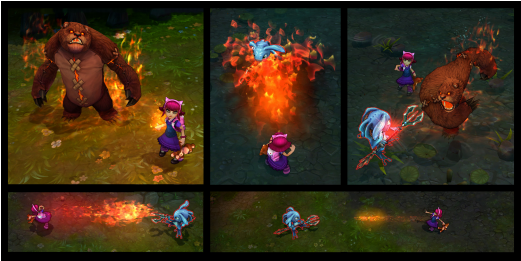
\includegraphics[scale = 0.90]{annie.PNG}\hspace{50mm}  
\end{center} 
\end{figure}\\ \\ \\ \\ \\ \\ \\ \\
\\Figura 1: Arriba a la izquierda “Tibbers”, arriba al centro “Incinerar”, Abajo a la izquierda “Desintegrar”\\
\\
Uno de estos champs es Annie, tu objetivo es ayudarla a determinar cuando podrá encadenar sus tres hechizos  ofensivos a un campeón enemigo. Los hechizos que conoce Annie son los siguientes:
\begin{itemize}
\item “Desintegrar” Annie lanza una bola de fuego imbuida de Maná a cualquier campeón en un area de $600u^1$ a su alrededor
\item “Incinerar” Annie lanza un abrasador cono de fuego, dañando a todos los enemigos de la zona. Este cono tiene  una apertura de 35° y además tiene un alcance de $500u$ (imagine una rebanada de pizza circular, con centro en Annie).
\end{itemize}
Puedes asumir de manera segura que no hay obstáculos entre Annie y su objetivo; además puedes despreciar el tiempo entre el lanzamiento de cada hechizo.
\\
\\
\textrm{\large Entrada}
\\
La primer línea de la entrada será un número $2 ≤ T ≤ 20$ que será el número de casos. Cada caso comenzará con tres números $0 ≤ A_x, A_y ≤ 10000$ y $1 ≤ Q ≤ 50$ donde los primeros dos son las coordenadas de Annie y el tercero el número de consultas para ese caso. Las siguientes $Q$ líneas tendrán dos números $0 ≤ E_x, E_y ≤ 10000$ que es la posición de el campeón objetivo. Se asegura que todos los números en la entrada son enteros.\\
\\
\\
\textrm{\large Salida}
\\
Para cada consulta deberas imprimir una línea que dirá “FULL COMBO” si puedes encadenar los 3 hechizos contra el campeón objetivo al mismo tiempo, si no puede, imprime “OUTPLAYED”.
\\
\\
\textrm{\large Entrada Ejemplo}
\\
2\\
0 1 1\\
490 2\\
23 4 1\\
700 900\\
\\
\\
\textrm{\large Salida Ejemplo}
\\
FULL COMBO\\
OUTPLAYED\\
\\
\\Sugerencias: 
$c_2 = a_2 + b_2$
\\
\textrm{\large Entendiendo el problema}\\
Dadas las posiciones de Annie y de un campeón en el plano, se nos pide saber si Annie es capaz de encadenar los tres hechizos que conoce al campeón enemigo. El problema nos dice que no habrá obstáculos entre ellos y que el lanzamiento de los hechizos es de manera instantánea.\\
\\
\textrm{\large Solución}\\
Lo que necesitamos para poder encadenar los tres hechizos es que la distancia entre Annie y el campeón sea menor o igual a 500$u$ ya que de éste modo los tres ataques pueden alcanzar al campeón.\\
\\
\textrm{\large Código}\\

\begin{minted}[breaklines,fontsize=\footnotesize,linenos]{cpp}
#include<bits/stdc++.h>
 
using namespace std;
 
#define FOR(i, a, b) for (int i = int(a); i < int(b); i++)
#define REP(i, a) for (int i = 0; i < int(a); i++)
#define INF 1000000000
typedef pair<int, int> ii;
typedef vector<int> vi;
typedef vector<ii> vii;
typedef long long ll;
typedef vector<bool> vb;
 
int casos, q;
ii annie, campeon;
 
int distancia_squared(ii u, ii v)
{
    return (u.first-v.first)*(u.first-v.first) + (u.second-v.second)*(u.second-v.second);
}
 
void querea()
{
    scanf("%d %d", &campeon.first, &campeon.second);
    int dis_squ = distancia_squared(annie, campeon);
    if( dis_squ <= 250000 )
        printf("FULL COMBO\n");
    else
        printf("OUTPLAYED\n");
 
}
 
void solve()
{
    scanf("%d %d", &annie.first, &annie.second);
    scanf("%d", &q);
    REP(i, q)
        querea();
}
 
int main()
{
    freopen("Annie.in", "r", stdin);
    freopen("Annie.out", "w", stdout);
    scanf("%d", &casos);
    while(casos--)
        solve();
    return 0;
}
\end{minted}
\newpage
%\hspace{1 cm}--- Linus
\hspace{5 cm}---\textrm{\large B- Colores\footnote[1]{Sergio Adrián Lagunas Pinacho - Grupo de Algoritmia Avanzada y Programación Competitiva}}\\
\\
\hspace{10 cm}---\textrm{\raggedright\normalsize  Límite de tiempo: 1 segundo}\\
\\ \\ \\ \\

\hfill
\begin{tabular}{@{}l@{}}
\textbf{Dificultad:} $\star$ \\
\textbf{Temas:} Ad-hoc \\
\textbf{Complejidad:} $O(1)$
\end{tabular}\\
\\
\\
Manuel Nicolás tiene éstos códigos de colores:\\
0 0 0 = Blanco\\
0 0 1 = Azul\\
0 1 0 = Rojo\\
0 1 1 = Morado\\
1 0 0 = Amarillo\\
1 0 1 = Verde\\
1 1 0 = Naranja\\
1 1 1 = Negro\\
\\Pero su amigo Mir Ist Kalt cambió los códigos, tal que los 1’s los volvió 0’s, y visceversa.\\
\\Tu trabajo es ayudar a Manuel Nicolás a decirle a qué color corresponde cada código cambiado.\\
\\
\\
\textrm{\large Entrada}
\\
La primera línea contendrá un entero $N (1 ≤ N ≤ 20)$, el número de casos de prueba. Las siguientes $N$ líneas tendrán $3$ dígitos, $di_1, di_2, di_3$ separados por un espacio $(0 ≤ d_{i1}, d_{i2}, d_{i3} ≤ 1)  (1 ≤ i ≤ N)$.
\\
\\
\textrm{\large Salida}
\\
Se tendrán que imprimir $N$ líneas, una por cada caso de prueba, todas terminando con salto de línea; cada línea tendrá el color correspondiente a su código.\\
\\
\\
\textrm{\large Entrada Ejemplo}
\\
4\\
0 0 0\\
1 1 1\\
0 0 1\\
0 1 1\\
\\
\\
\textrm{\large Salida Ejemplo}
\\
Negro\\
Blanco\\
Naranja\\
Amarillo\\
\\
\textrm{\large Entendiendo el problema}\\
Nos dan un diccionario de colores cuyo código está en binario. En el problema se te da el código alterado (intercambiando unos y ceros) de un color y se te pide imprimir el color correspondiente del código original.
\\
\textrm{\large Solución}\\
Directa.\\
\\
\textrm{\large Código}\\

\begin{minted}[breaklines,fontsize=\footnotesize,linenos]{cpp}
#include<iostream>

using namespace std;

typedef vector<int> vi;
typedef vector<pair<int,int> > vii;
typedef vector<vi> vvi;
#define rep(a,b) for(int a=0;a<b;a++)
#define For(a,b,c) for(int a=b;a<c;a++)
int main()
{
    std::ios_base::sync_with_stdio(false);
    int n,a,b,c;
    string v[8] = {"Negro","Naranja","Verde","Amarillo","Morado","Rojo","Azul","Blanco"};
    cin>>n;
    rep(i,n){
        cin>>a>>b>>c;
        cout<<v[4*a + 2*b + c]<<endl;
    }
    return 0;
}
\end{minted}
\newpage
%\hspace{1 cm}--- Linus
\hspace{5 cm}---\textrm{\large C - CandyLand\footnote[1]{David Felipe Castillo Velázquez - Grupo de Algoritmia Avanzada y Programación Competitiva}}\\
\\
\hspace{10 cm}---\textrm{\raggedright\normalsize  Límite de tiempo: 1 segundo}\\
\\

\hfill
\begin{tabular}{@{}l@{}}
\textbf{Dificultad:} $\star$ \\
\textbf{Temas:} Sliding window \\
\textbf{Complejidad:} $O(n)$
\end{tabular}\\
\\
Mágicamente has sido transportado a la asombrosa tierra de CandyLand, donde hay tantos dulces de tantos sabores como nunca habías imaginado. Siendo un fanático de los dulces no puedes contener la felicidad y empiezas a probar todos los dulces existentes y asignas a cada dulce un valor de sabrosidad.\\ \\ Sin embargo no todo puede ser tan perfecto, tu tiempo en CandyLand está a punto de acabar y serás transportado de regreso a tu vida cotidiana, pero no quieres irte con las manos vacías.\\
\\Enfrente de ti hay una línea con $1 ≤ N ≤ 106$ dulces numerados del $1$ al $N$, donde al i-ésimo dulce le has asignado un valor de sabrosidad $−100 ≤ S_i ≤ 100$. Y convenientemente tienes a tu disposición un brazo robótico capaz de agarrar exactamente $1 ≤ K ≤ 103$
, $K ≤ N$ dulces consecutivos de dicha línea, y una computadora.\\ \\Debido a que hay algunos dulces que no te gustan tanto, quieres agarrar $K$ dulces tales que la suma de su valor de sabrosidad sea el máximo posible. Como la cantidad de dulces es muy grande necesitas hacer un programa que te diga cuál es el índice del primer dulce de la izquierda que debe agarrar el brazo robótico para lograr tu objetivo.\\
\\
\\
\textrm{\large Entrada}
\\
La primer línea contendrá el número $1 ≤ T ≤ 50$ de casos. Para cada caso habrá dos líneas.\\ \\La primer línea de cada caso contendrá dos enteros $N$ y $K$. La segunda línea de cada caso contendrá $N$ enteros Si, $1 ≤ i ≤ N$.
\\
\\
\textrm{\large Salida}
\\
Para cada caso deberás imprimir dos enteros en una línea, el índice del primer dulce de la izquierda que debe agarrar el brazo robótico para lograr tu objetivo, si hay más de una opción imprime el que tenga el menor índice, y la suma máxima del valor de sabrosidad que puedes conseguir.\\
\\Nota\\
El brazo robótico tiene que agarrar exactamente $K$ dulces.
\\
\\
\textrm{\large Entrada Ejemplo}
\\
1\\
10 4\\
1 -5 5 10 -1 3 -2 -3 9 4\\
\\
\\
\textrm{\large Salida Ejemplo}
\\
3 17\\
\\
\textrm{\large Entendiendo el problema}\\
El problema se reduce a: dado un arreglo de $n$ enteros, encontrar el subarreglo de tamaño exactamente $k$, tal que la suma del subarreglo sea máxima.\\
\\
\textrm{\large Solución}\\
La solución $O(nk)$ es demasiado lenta para este problema. Sea \texttt{a[]} el arreglo de enteros. Si declaramos un arreglo \texttt{v[i]} $:= \sum_{j=1}^i$ \texttt{a[j]}, entonces la suma del subarreglo de tamaño $k$ empezando en la posición $i$ es: \texttt{v[i+k]-v[i-1]}. Con esta observación tenemos una solución $O(n)$.\\
\\
\textrm{\large Código}\\

\begin{minted}[breaklines,fontsize=\footnotesize,linenos]{cpp}
#include <iostream>
#include <cstdio>
#include <cstring>
#include <algorithm>
 
#define For(i, a, b) for(int i=a; i<b; ++i)
#define INF (1<<30)
 
using namespace std;
 
int v[1000005];
 
int main()
{
    int T;
    scanf("%d", &T);
 
    while (T--)
    {
        int N, K;
        scanf("%d %d", &N, &K);
 
        int res = -INF, ind = 1;
        For(i, 1, N+1)
        {
            scanf("%d", &v[i]);
            v[i] += v[i-1];
        }
 
        For(i, K, N+1)
            if (v[i] - v[i-K] > res)
                res = v[i]-v[i-K], ind = i-K+1;
 
        printf("%d %d\n", ind, res);
    }
 
    return 0;
}
\end{minted}
\newpage
%\hspace{1 cm}--- Linus
\hspace{5 cm}---\textrm{\large D - Raíces Digitales\footnote[1]{Sergio Adrián Lagunas Pinacho - Grupo de Algoritmia Avanzada y Programación Competitiva}}\\
\\
\hspace{10 cm}---\textrm{\raggedright\normalsize  Límite de tiempo: 1 segundo}\\
\\

\hfill
\begin{tabular}{@{}l@{}}
\textbf{Dificultad:} $\star \star$ \\
\textbf{Temas:} Ad-hoc \\
\textbf{Complejidad:} $O(k)$
\end{tabular}\\
\\
\\
Recientemente Manuel Nicolás León descubrió qué es la raáz digital, y decidió compartir su conocimiento contigo.\\
Digamos que $S(n)$ es la suma de los dígitos de $n$, por ejemplo, $S(4089) = 4 + 0 + 9 + 8 = 21$, entonces la raíz
digital del número $n$ es:
\begin{enumerate}
\item $rd(n) = S(n)  		si S(n) < 10$
\item $rd(n) = rd(S(n)) 	si S(n) ≥ 10$
\end{enumerate}
Por ejemplo, $rd(4098) = rd(21) = rd(3) = 3$.
\\ \\Manuel le tiene miedo a los números grandes, por eso los números con los que trabajará serán a lo mas 10100.\\
\\Para todos esos números, Manuel ha probado que \\$rd(n) = S(S(S(S(n))))(n ≤ 10^100)$.\\
\\Ahora Manuel quiere encontrar números rápidamente dada su raiz digital. El problema es que todavía no ha aprendido a hacer lo que te va a preguntar. Tu tarea es, dados los núumeros $k$ y $d$, encontrar números exactamente de $k$ dígitos (sin ceros al principio), con su raíz digital igual a $d$.
\\
\\
\textrm{\large Entrada}
\\
La primera línea tendrá un número $T (T ≤ 500)$ que representa el número de casos de prueba.\\
Las siguientes $T$ líneas contendrán los casos de prueba, cada caso tendrá 2 números, $k$ y $d (1 ≤ k ≤ 100; 1 ≤ d ≤ 9)$.
\\
\\
\textrm{\large Salida}
\\
Se imprimirán $2T$ líneas, $2$ por cada caso de prueba: la primera línea de cada caso de prueba tendrá el número $n$ más grande tal que $rd(n) = d$, y el número de dígitos de $n$ sea igual a $k$; la segunda línea de cada caso de prueba tendrá el número $n$ más chico tal que $rd(n) = d$, y el número de dígitos de $n$ sea igual a $k$.\\
\\Puedes tener la seguridad de que dichos números siempre existen, y son únicos.
El primer dígito de cada número impreso no tiene que ser un $0$.
\\
\\
\textrm{\large Entrada Ejemplo}
\\
2\\
1 3\\
1 7\\
\\
\\
\textrm{\large Salida Ejemplo}
\\
3\\
3\\
7\\
7\\
\\
\textrm{\large Entendiendo el problema}\\
En el problema se define $S(n)$ como la suma de los dígitos de $n$ y
\[
rd(n) =
\left\{
	\begin{array}{ll}
		S(n)     & \mbox{si } S(n) < 10 \\
		rd(S(n)) & \mbox{si } S(n) \geq 10   \\
	\end{array}
\right.
\]
Se nos da $1 \leq k \leq 100$ y $1 \leq d \leq 9$, y se nos pide encontrar el número más pequeño $min$ y el número más grande $max$ tales que $rd(min) = rd(max) = d$ y tanto $min$ como $max$ contengan $k$ dígitos.\\ 
\\
\textrm{\large Solución}
Éstos dos números se construyen de la siguiente manera:
\begin{align*}
& min = (1)(\underbrace{0\ ...\ 0 }_{k-2})(d-1) \\
& max = (\underbrace{9\ ...\ 9}_{k-1})(d)
\end{align*}
\\
\textrm{\large Código}\\

\begin{minted}[breaklines,fontsize=\footnotesize,linenos]{java}
import java.util.*;
import java.io.*;
 
class D
{
    public static void main(String[] args)
    {
        MyScanner sc = new MyScanner();
        int T = sc.nextInt();
 
        while (T-- > 0)
        {
            int k = sc.nextInt(), d = sc.nextInt();
 
            for(int i = 0; i < k-1; i++)
                System.out.print(9);
            System.out.println(d);
 
            if (k > 1)
                System.out.print(1);
            for(int i = 1; i < k-1; i++)
                System.out.print(0);
            if (k > 1)
                System.out.println(d-1);
            else
                System.out.println(d);
        }
    }
};
\end{minted}
\newpage
%\hspace{1 cm}--- Linus
\hspace{5 cm}---\textrm{\large E - Buscando Asiento\footnote[1]{Sergio Adrián Lagunas Pinacho - Grupo de Algoritmia Avanzada y Programación Competitiva}}\\
\\
\hspace{10 cm}---\textrm{\raggedright\normalsize  Límite de tiempo: 1 segundo}\\
\\
\hfill
\begin{tabular}{@{}l@{}}
\textbf{Dificultad:} $\star \star$ \\
\textbf{Temas:} Ad-hoc \\
\textbf{Complejidad:} $O(1)$
\end{tabular}\\
\\
\\
Manuel Nicolás León es un chico muy especial... cuando va a conferencias le gusta que la silla de su izquierda y la silla de su derecha estén desocupadas.\\
\\Este año irá a una conferencia a la cuál irán sólo chicos igual de especiales que él (que les gusta que las sillas adyacentes a la suya estén desocupadas). Para el problema tienes que decir si es posible que todos los chicos, incluyendo Manuel, estén a gusto, ésto es, que todos los chicos tengan libres las sillas adyacentes a la suya.\\
\\
\\
\textrm{\large Entrada}
\\
La primera línea tendrá un número $T$ que representa el número de casos de prueba.\\
\\Las siguientes $T$ líneas contendrán los casos de prueba, cada caso tendrá 2 números, $A$ y $B (1 ≤ A ≤ B ≤ 500)$ indicando el número de chicos, y el número de sillas disponibles respectivamente.\\
\\Los chicos escogen las sillas uno por uno, escogiendo una silla que tenga sus 2 sillas adyacentes desocupadas (Si es una de las sillas de la orilla, basta con que la única silla adyacente que tiene est´e desocupada).\\
\\Tu tarea es, dadas éstas condiciones, decir si los chicos se sentirán a gusto o no.
\\
\\
\textrm{\large Salida}
\\
Se imprimirán $T$ líneas, una por cada caso de prueba, con alguna de las siguientes palabras: “Si” si siempre es posible que todos los chicos estén a gusto, “No” si es imposible que todos los chicos estén a gusto, o “Tal vez” si depende de cómo se vayan sentando los chicos.\\
\\
\\
\\
\textrm{\large Entrada Ejemplo}
\\
3\\
1 3\\
2 3\\
3 3\\
\\
\textrm{\large Salida Ejemplo}
\\
Si\\
Tal vez\\
No\\
\\
\textrm{\large Entendiendo el problema}\\
El problema nos dice que hay $A$ niños que se quieren sentar en $B$ asientos, sin embargo cada uno de los niños quiere sentarse en un asiento tal que sus dos vecinos estén desocupados. Los niños van sentándose uno por uno escogiendo cualquier asiento que cumpla con los requerimientos. Debemos ver si siempre es posible que estén agusto independientemente de cómo se vayan sentado (caso ``Si''), si depende de los asientos que escojan (caso ``Tal vez''), o sin importar que asientos escojan no es posible que estén agustos (caso ``No'').\\ 
\\
\textrm{\large Solución}\\
\begin{enumerate}
\item Caso ``No''. Si $A > \Big\lceil \frac{B}{2} \Big\rceil$. Pues la mejor forma en que se pueden ir sentando es dejando un espacio de separación, si así no es posible sentarlos, entonces no hay forma de que estén agusto.
\item Caso ``Si''. Si $A \leq \Big\lceil \frac{B}{3} \Big\rceil$. La ``peor'' forma en la que se pueden acomodar los niños es si cada uno se coloca a dos asientos de separación de sus vecinos, ya que si se sientan a un asiento de separación sería la forma más ``compacta'', y si se sientan a más de dos, entonces un tercer niño puede sentarse en medio de ellos. Ésto se vería de la siguiente forma:
\[
...010\underbrace{010}_{3}010...
\]

Por lo tanto se puede apreciar que cada niño ``cubre'' tres asientos.
\item Caso ``Tal vez''. Si $\Big\lceil \frac{B}{3} \Big\rceil < A \leq \Big\lceil \frac{B}{2} \Big\rceil$
\end{enumerate}
\textrm{\large Código}\\

\begin{minted}[breaklines,fontsize=\footnotesize,linenos]{java}
import java.util.Scanner;
 
class E
{
    public static void main(String[] args)
    {
        Scanner sc = new Scanner(System.in);
 
        int T = sc.nextInt();
         
        while (T-- > 0)
        {
            int n = sc.nextInt(), s = sc.nextInt();
 
            int limNo = s % 2 == 0 ? s / 2 : s / 2 + 1;
            int limSi = s % 3 == 0 ? s / 3 : s / 3 + 1;
 
            if (n > limNo)
                System.out.println("No");
            else if (n <= limSi)
                System.out.println("Si");
            else
                System.out.println("Tal vez");
        }
    }
};
\end{minted}
\newpage
%\hspace{1 cm}--- Linus
\hspace{5 cm}---\textrm{\large F - Fibonacci\footnote[1]{Sergio Adrián Lagunas Pinacho - Grupo de Algoritmia Avanzada y Programación Competitiva}}\\
\\
\hspace{10 cm}---\textrm{\raggedright\normalsize  Límite de tiempo: 1 segundo}\\
\\

\hfill
\begin{tabular}{@{}l@{}}
\textbf{Dificultad:} $\star$ \\
\textbf{Temas:} Ad-hoc \\
\textbf{Complejidad:} $O(1)$
\end{tabular}\\
\\
\\Manuel Nicolás León es un chico muy curioso, tanto que durante una de sus clases se le ocurrió una sucesión de dígitos parecida a la de Fibonacci, la cuál empieza con 2 dígitos, 1 y 1, y para la cual cual(es)quiera dígito(s) que se le vaya a añadir es igual a los dígitos que equivalen a la suma de los valores numéricos de los 2 dígitos anteriores,
así el tercer dígito sería $1+1=2$, el cuarto sería $1+2=3$, el quinto $2+3=5$, el sexto $3+5 = 8$, y así sucesivamente.\\
\\Lo interesante de ésta sucesión empieza del dígito $7$ en adelante; dado que $5+8 = 13$, los dígitos $7$ y $8$ serían el $1$ y el $3$ respectivamente; el dígito que ocuparía la posición $9$ sería $1+3=4$, y así sucesivamente, dando lugar a algo como ésto:\\
\\
\hspace{5 cm}\textrm{112358134...}
\\
\\Manuel Nicolás León se pregunta si hay alguna forma de saber cualquier dígito de la sucesi´on con ayuda de un
programa, para lo cu´al te ha pedido tu ayuda: tienes que programarlo.
\\
\\
\textrm{\large Entrada}
\\
La primera línea contendrá un entero $N (1 ≤ N ≤ 20)$, el número de casos de prueba. Las siguientes $N$ líneas tendrán un número entero positivo Si $(1 ≤ Si ≤ 109)$  $(1 ≤ i ≤ N)$ que representa el dígito requerido.
\\
\\
\textrm{\large Salida}
\\
Se tendrán que imprimir $N$ líneas, una por cada caso de prueba, todas terminando con salto de línea; cada línea tendrá un dígito $D_i (0 ≤ D_i ≤ 9)$  $(1 ≤ i ≤ N)$ que representa el dígito que está en la posición Si requerido.\\
\\
\\
\textrm{\large Entrada Ejemplo}
\\
6\\
1\\
2\\
3\\
7\\
8\\
9\\
\\
\\
\textrm{\large Salida Ejemplo}
\\
1\\
1\\
2\\
1\\
3\\
4\\
\\
\textrm{\large Entendiendo el problema}\\
En este caso se nos da una cadena de dígitos $F$ cuya construcción se parece a la sucesión de Fibonacci. La forma de construirla es sumar los dos últimos dígitos de la cadena y concatenar el resultado. Los primeros dígitos de la cadena son los siguientes:
\[
\underbrace{1123581347}_{10}112...
\]
Y se nos pide saber cuál es el $n$-ésimo dígito de la cadena $F$.\\
\\
\textrm{\large Solución}\\
Los dígitos señalados siempre se van a repetir, debido a que se toman los dos últimos dígitos para construir los siguientes. Por lo tanto sólo debemos guardar los diez primeros dígitos y el $n$-ésimo dígito de $F$ será $F[n\%10]$.\\
\\
\textrm{\large Código}\\

\begin{minted}[breaklines,fontsize=\footnotesize,linenos]{cpp}
#include <bits/stdc++.h>

using namespace std;
typedef vector<int> vi;
typedef vector<pair<int,int> > vii;
typedef vector<vi> vvi;
#define rep(a,b) for(int a=0;a<b;a++)
#define For(a,b,c) for(int a=b;a<c;a++)
int main()
{
    std::ios_base::sync_with_stdio(false);
    int n,x,v[10]={1,1,2,3,5,8,1,3,4,7};//1123581347
    cin>>n;
    while(n--)
    {
        cin>>x;
        x--;
        printf("%d\n",v[x%10]);
    }
    return 0;
}
\end{minted}
\newpage
%\hspace{1 cm}--- Linus
\hspace{5 cm}---\textrm{\large G - Código\footnote[1]{Maximiliano Luna Vera - Grupo de Algoritmia Avanzada y Programación Competitiva}}\\
\\
\hspace{10 cm}---\textrm{\raggedright\normalsize  Límite de tiempo: 1 segundo}\\

\hfill
\begin{tabular}{@{}l@{}}
\textbf{Dificultad:} $\star$ \\
\textbf{Temas:} Ad-hoc \\
\textbf{Complejidad:} $O(NM)$
\end{tabular}
\\
\\
Mau es un chico al que le encanta descifrar c´odigos. Recientemente un amigo suyo le contó acerca de un nuevo código que ha estado desarrollando. Este código consiste en colocar el mensaje a codificar sin espacios en una cuadrícula de $M × N$, siendo $M$ el número de renglones y $N$ el número de columnas. \\Luego se rota la cuadrícula 90 grados. Así, al leer normalmente el mensaje colocado en la cuadrícula, éste será incomprensible.\\
\\Un ejemplo se muestra en la siguiente imagen:
\begin{figure}[h!] 
\begin{center} 
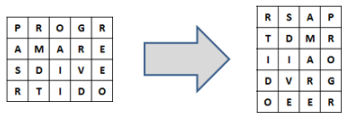
\includegraphics[scale = 0.90]{fig.PNG}\hspace{50mm}  
\end{center} 
\end{figure}
\\Mau puede decodificar este código, pero no lo suficientemente rápido, por eso te ha pedido ayuda a ti, su amigo programador, para implementar un programa que descifre este tipo de códigos.\\
\\Tu tarea será, dado el mensaje codificado, imprimir el mensaje original que fue colocado en la cuadrícula.
\\
\\
\textrm{\large Entrada}
\\
La primera línea contiene un entero $T(1 ≤ T ≤ 50)$, el número de casos de prueba. Para cada uno de los siguientes $T$ casos siguen $2$ líneas.\\
\\La primera de ellas contiene dos enteros $M$ y $N$,$(1 ≤ M, N ≤ 50)$, que representan el número de renglones y columnas respectivamente en las que esta colocado el mensaje original.\\
\\La segunda contiene el mensaje codificado, de tamaño $M × N$ el cual podrá estar formado de letras mayúsculas, letras minúsculas y números.
\\
\\
\textrm{\large Salida}
\\
Para cada caso imprime solo una línea que debe contener el mensaje original, con la distinción de mayúsculas y minúsculas.
\\
\\
\textrm{\large Entrada Ejemplo}
\\
1\\
4 5\\
RSAPTDMRIIAODVRGOEER\\
\\
\\
\textrm{\large Salida Ejemplo}
\\
PROGRAMARESDIVERTIDO\\
\\
\textrm{\large Entendiendo el problema}\\
En el problema se nos da una $S$ cadena de tamaño $N\times M$ codificada. La forma en que se codifico la cadena fue metiéndola en una matriz de tamaño $N \times M$ y rotarla 90 grados en sentido del reloj. Después de ésto se agarran los caracteres dentro de la matriz rotada en orden de arriba hacia abajo y de izquierda a derecha. La tarea consiste en decodificar el mensaje.\\
\\
\textrm{\large Solución}\\
 Para hacerlo hay que meter la cadena en una matriz de $M \times N$, rotarla 90 grados en sentido contrario al reloj e imprimir los caracteres en el mismo orden. Esto se puede lograr con puro manejo de índices.\\
\\
\textrm{\large Código}\\

\begin{minted}[breaklines,fontsize=\footnotesize,linenos]{cpp}
#include<iostream>
#include<cstdio>
#include<cstdlib>
#include<string>
using namespace std;
int main()
{
    int t,m,n;
    string s;
    cin>>t;
    while(t--)
    {
        cin>>m>>n;
        cin>>s;
        for(int i=m-1;i>=0;i--)
            for(int j=0;j<n;j++)
                cout<<s[i+m*j];
        cout<<endl;
    }
 
    return 0;
}
\end{minted}
\newpage
\section{concurso de programación}{\large XIII Semana de MAC}\\
\\
\hspace{5 cm}---\textrm{\large D - El Desafío\footnote[1]{Kenny Yahir Méndez Ramírez - Grupo de Algoritmia Avanzada y Programación Competitiva}}\\
\\
\hspace{10 cm}---\textrm{\raggedright\normalsize  Límite de tiempo: 1 segundo}\\
\\

\hfill
\begin{tabular}{@{}l@{}}
\textbf{Dificultad:} $\star$ \\
\textbf{Temas:} Matemáticas \\
\textbf{Complejidad:} $O(1)$
\end{tabular}\\
\\
Fer y Dianita son grandes amigas, están la mayor parte del tiempo juntas y siempre se la pasan muy bien. Por alguna extraña razón a Fer le gustan los números naturales que son múltiplos del 3 y a Dianita los que son múltiplos del 5.\\
\\Entre las cosas que disfrutan hacer es comer frituras, pero a su amigo Kenny no le agrada, (el piensa que no son para nada saludables), así que un día deliveradamente ellas le propusieron lo siguiente: “Si nos dices cuál es la suma de nuestros números favoritos que son menores a $N$, hoy no comeremos papitas, más sin embargo si te equivocas, tú nos las tendrás que invitar”. \\ \\Kenny se preocupa por sus amigas, así que aceptó el desafío y no quiere equivocarse (además también es algo tacaño); la cuestión es que no es muy bueno haciendo cálculos tan rápido. ¿Podrías ayudar a nuestro amigo Kenny diciéndole cuál es la respuesta correcta dado un cierto $N$?\\
\\
\textrm{\large Entrada}
\\
La primera línea de entrada contendrá un entero $C$, que indica el número de casos de prueba. En las siguientes $C$ lineas aparecerá un entero $N$.\\
\\
\textrm{\large Salida}
\\
Para cada caso de entrada deberás imprimir una sola línea que contenga un entero, la respuesta al problema
planteado.\\
\\Restricciones fácil
$C = 100$\\
$1 ≤ N ≤ 50000$\\
1\\
\\Restricciones difícil
C = 100000\\
$1 ≤ N ≤ 109$\\
\\
\\
\textrm{\large Entrada Ejemplo}
\\
3\\
10\\
15\\
100\\
\\
\\
\textrm{\large Salida Ejemplo}
\\
23\\
45\\
2318\\
\\Notas: 
Se asegura que la respuesta cabe en un entero de 64 bits.\\
\\
\textrm{\large Entendiendo el problema}
Dado un entero $N$ se quiere determinar la suma de los múltipos de 3 y 5 que son menores a $N$. No se deben sumar dos o más veces el mismo número.\\
\\
\textrm{\large Solución}
\\
\textrm{\large Caso Fácil}\\
Para el caso fácil podemos correr 2 ciclos que verifiquen qué números son divisibles por 3 y por 5 respectivamente, sumarlos, incrementar \texttt{i} en 3, 5, y en alguno de los 2 ciclos no contar a aquellos números que son múltiplos de ambos, ya que estaríamos contándolos 2 veces. Esta idea corre en $O(n)$. Lo cual es bueno si $n$ no es ``grande''.\\
\\
\textrm{\large Caso Difícil}\\
Para el caso dificil, la idea anterior no funcionaría ya que las restricciones obligarían a usar un ciclo demasiado grande, entonces usamos una idea mejor:

Pensemos en la suma de los primeros $n$ múltiplos de 3 como:
\begin{eqnarray*}
3 + 6 + 9 + \hdots + 3n\\
3 (1 + 2 + 3 + \hdots +n)
\end{eqnarray*}
Nos percatamos que el segundo factor de la expresión anterior es la suma de los primeros $n$ naturales, entonces queda como:
\begin{eqnarray*}
3 \frac{n(n+1)}{2}
\end{eqnarray*}
De manera similar para el caso de 5:
\begin{eqnarray*}
5 \frac{n(n+1)}{2}
\end{eqnarray*}

Entonces la suma de las expresiones anteriores es casi lo que queremos, esto porque en cada una de ellas se está contemplando los múltiplos de 5 y 3 al mismo tiempo, así que solo necesitamos eliminar una vez la suma de éstos:
\begin{eqnarray*}
15 \frac{n(n+1)}{2}
\end{eqnarray*}
Ahora ¿cómo encontramos los primeros $n$ múltiplos menores a $N$?, fácil, basta con hacer una división entera de $N-1$ entre el divisor deseado. De esta manera  nuestro programa se vería de la siguiente forma:
\\
\textrm{\large Código}
\begin{minted}[breaklines,fontsize=\footnotesize,linenos]{cpp}
#include <iostream>
#include <cstdio>
#define For(x,a,b) for(int x=a; x<b; x++)
using namespace std;

typedef long long ll;

ll mtres(ll n){ll r = n/3; return (r*(r+1)/2)*3;}
ll mcinco(ll n){ll r= n/5; return (r*(r+1)/2)*5;}
ll mquince(ll n){ll r= n/15; return (r*(r+1)/2)*15;}

int main()
{
	int T,N;
	
	scanf("%d",&T);
	
	For(j,0,T)
	{
		scanf("%d",&N);
		
		printf("%lld\n",mtres(N-1)+mcinco(N-1)-mquince(N-1));
	}
	return false;
}
\end{minted}
\newpage
%\hspace{1 cm}--- Linus
\hspace{5 cm}---\textrm{\large A - Avería\footnote[1]{Maximiliano Vera Luna - Grupo de Algoritmia Avanzada y Programación Competitiva}}\\
\\
\hspace{10 cm}---\textrm{\raggedright\normalsize  Límite de tiempo: 1 segundo}\\
\\

\hfill
\begin{tabular}{@{}l@{}}
\textbf{Dificultad:} $\star$ \\
\textbf{Temas:} Matemáticas \\
\textbf{Complejidad:} $O(\log \min(a, b))$
\end{tabular}\\
\\Marta es una chica a la que le encanta conducir, ella es muy hábil al volante y conduce su auto a todas horas y a todos lugares en cualquier tipo de clima. Debido a esto y a la lluvia, el pobre automóvil de Marta ha sufrido una pequeña avería.\\
\\Durante estas fuertes lluvias, los limpiaparabrisas de su auto se han descompuesto. Ahora cada uno de los dos limpiaparabrisas realiza su recorrido (ida y vuelta) en tiempos distintos, lo que ocasiona que si ella los detiene cuando alguno de los dos llega al final de su primer recorrido, el otro se encuentre obstruyendo su vista y la distraiga, por lo que podría tener un accidente.\\
\\Por lo tanto Marta te ha pedido ayuda a tí. Dado el tiempo en segundos en que cada uno de los limpiaparabrisas de su auto hace su recorrido, calcula el mínimo de segundos que deben pasar para que ambos regresen a su posición de partida. Toma en cuenta que su posición de partida es la misma que tienen los limpiaparabrisas en buenas condiciones cuando están apagados.\\
\begin{figure}[h!] 
\begin{center} 
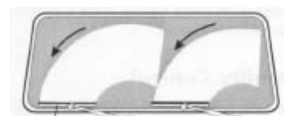
\includegraphics[scale = 0.90]{pa.PNG}\hspace{50mm}  
\end{center} 
\end{figure}
\\Entrada
\\La primera línea de entrada contiene un entero $T$, el número de casos de prueba. Las siguientes $T$ líneas contienen dos enteros diferentes $A$ y $B$, que representan los segundos que tarda cada uno de los limpiaparabrisas en su recorrido.
\\
\\
\textrm{\large Salida}
\\
Para cada caso de prueba imprime una sola línea con un entero que represente el reultado del calculo explicado anteriormente.
\\
\\
\textrm{\large Entrada Ejemplo}
\\
2\\
3 5\\
16 12\\
1\\
\\
\\
\textrm{\large Salida Ejemplo}
\\
15\\
48\\
\\Restricciones
\\Fácil
$1 ≤ T ≤ 100$
$1 ≤ A, B ≤ 500$ con $A$ diferente de $B$.
\\Difícil
$1 ≤ T ≤ 10000$
$1 ≤ A, B ≤ 40000$ con $A$ diferente de $B$.\\
\textrm{\large Entendiendo el problema}
Se tienen dos limpiaparabrisas, los cuales realizan un ciclo en $a$ y $b$ segundos, respectivamente. Se dice que los limpiaparabrisas empiezan a funcionar al mismo tiempo, en la misma posición, y se quiere saber en cuánto tiempo volveran en encontrarse en la misma posición por primera vez.\\

\textrm{\large Solución}\\

Lo que buscamos son dos números $k$, $q$ tal que $ak = bq$, y que $ak$ sea mínimo. La respuesta es $ak$. Es fácil ver que $ak = bq = lcm(a, b)$ nos minimiza este valor.\\

\textrm{\large Caso Fácil}\\
Para el caso fácil, se puede ir aumentando por si misma una de las variables hasta que la otra la divida exactamente, esto es el primer momento en el que ambos se encuentran en su punto de inicio otra vez.\\

\textrm{\large Caso Difícil}\\
Para el caso difícil, las restricciones no nos permiten hacer el mismo cálculo debido al numero de casos de prueba.\\

La solución es ver que el Mínimo Común Multiplo de dos números se puede calcular de la siguiente forma:

$$\textnormal{MCM}(a,b) = \frac{ab}{\textnormal{MCD}(a, b)}$$

donde MCD es el máximo común divisor de los dos números.

Ahora, para calcular el Máximo Común Divisor de dos números eficientemente, podemos utilizar el algoritmo de Euclides.

La siguiente rutina basada en ese algoritmo nos devuelve el $\textnormal{MCD}(a, b)$ y la calcula en $O(\log n)$ donde $n$ es el máximo de $a$ y $b$.\\

\textrm{\large Código}\\
\begin{minted}[breaklines,fontsize=\footnotesize,linenos]{cpp}
#include<iostream>
#include<algorithm>
using namespace std;
 
int gcd(int a, int b) { return b == 0 ? a : gcd(b, a % b); }
int lcm(int a, int b) { return a * (b / gcd(a, b)); }
 
int main()
{
    int n, a, b;
    cin >> n;
    for(int i = 0; i < n; i++)
    {
        cin >> a >> b;
        cout << lcm(a, b) << endl;
    }
    return 0;
}
\end{minted}
\newpage
%\hspace{1 cm}--- Linus
\hspace{5 cm}---\textrm{\large C - Conejos\footnote[1]{David Felipe Castillo Velázquez - Grupo de Algoritmia Avanzada y Programación Competitiva}}\\
\\
\hspace{10 cm}---\textrm{\raggedright\normalsize  Límite de tiempo: 1 segundo}\\
\\

\hfill
\begin{tabular}{@{}l@{}}
\textbf{Dificultad:} $\star \star \star \star$ \\
\textbf{Temas:} Matemáticas \\ Exponenciación de matrices \\
\textbf{Complejidad:} $O(\log n)$
\end{tabular}\\
\\
Johanna es una brillante matemática amante de los conejos que recientemente consiguió una pareja de bellos conejos a los que nombró Fibonacci y Lucas (se desconoce cuál de los dos conejos es la hembra).\\ \\Al cabo de unos meses los pequeños conejos se reprodujeron y Johanna empezó a darse cuenta que el número de parejas de conejos que habían cada mes eran: $1, 1, 2, 3, 5, 8, ...$ y no tardó en deducir que el número de parejas $f_n$ en el mes $n$ estaba
dada por la recurrencia $f_n = f_{n−1} + f_{n−2}$.\\
\\Johanna tiene dos hermanas menores, Isabella y Karen, quienes también aman a los conejos, y es por eso que Johanna ha decidido regalarles todos sus conejos, sin embargo no quiere que se peleen entre ellas, por lo tanto necesita regalarles exactamente la misma cantidad de parejas de conejos a cada una.\\
\\Para poderles regalar la misma cantidad de pares de conejos a Isabella y Karen, Johanna necesita que el número total de parejas de conejos sea par, así que a ella sólo le interesan los meses en lo que esto sucede y a dichos meses los ha nombrado conejo-meses. Así en los primeros 4 conejo-meses el número de parejas de conejos son: 2, 8, 34
y 144.\\ \\Johanna necesita tu ayuda para determinar cuántos conejos tendrá en el N-ésimo conejo-mes. \\Como este número puede ser muy grande Johanna te pide que imprimas el resultado módulo $109 + 7 (1000000007)$.
\\
\\
\textrm{\large Entrada}
\\
La primera línea contiene un entero $t$, el número de casos de prueba. Las siguientes $t$ líneas contienen un entero $N$
\\
\\
\textrm{\large Salida}
\\
Para cada caso de prueba debes imprimir, en una línea, el número de pares de conejos que tendrá Johanna en el N-ésimo conejo-mes.\\
\\Restricciones
\\Fácil
t = 100\\
$1 ≤ N ≤ 1000$\\
\\Difícil
t = 1000\\
$1 ≤ N ≤ 1018$\\
\\
\\
\textrm{\large Entrada Ejemplo}
\\
5\\
1\\
2\\
5\\
10\\
43\\
\\
\\
\textrm{\large Salida Ejemplo}
\\
2\\
8\\
610\\
832040\\
461493940\\
\\Notas
Recordar que:\\
$(a + b) \%M = (a \%M) + (b \%M)$
$(a × b) \%M = ((a \%M) × (b \%M)) \%M$\\
\\
\textrm{\large Entendiendo el problema}\\
El problema consistía en encontrar el $n$-ésimo fibonacci par. \\

\textrm{\large Solución}\\
Sea $f_n = 4f_{n-1} + f_{n-2}$, con $f_1 = 2$ y $f_2 = 8$. Mostraremos que $f_n$ nos da el $n$-ésimo fibonacci par. Dado que cada tercer elemento de la sucesión de fibonacci es par, basta con probar que $fib_n = 4fib_{n-3} + fib_{n-6}$.
\begin{align*}
fib(n) & = fib_{n-1} + fib_{n-2} \\
       & = fib_{n-2} + 2fib_{n-3} + fib_{n-4} \\
       & = 3fib_{n-3} + 2fib_{n-4} \\
       & = 3fib_{n-3} + fib_{n-4} + fib_{n-5} + fib_{n-6} \\
       & = 4fib_{n-3} + fib_{n-6}
\end{align*}
Sea $f_n = 4f_{n-1} + f_{n-2}$, con $f_1 = 2$ y $f_2 = 8$. Mostraremos que $f_n$ nos da el $n$-ésimo fibonacci par. Dado que cada tercer elemento de la sucesión de fibonacci es par, basta con probar que $fib_n = 4fib_{n-3} + fib_{n-6}$.

\begin{align*}
fib(n) & = fib_{n-1} + fib_{n-2} \\
       & = fib_{n-2} + 2fib_{n-3} + fib_{n-4} \\
       & = 3fib_{n-3} + 2fib_{n-4} \\
       & = 3fib_{n-3} + fib_{n-4} + fib_{n-5} + fib_{n-6} \\
       & = 4fib_{n-3} + fib_{n-6}
\end{align*} 

Con esto sólo necesitamos calcular $f_n$. 
\\
\textrm{\large Caso Fácil}\\
Para el caso fácil era posible hacerlo en $O(n)$ con un \textbf{for}.\\
\\
\textrm{\large Caso Difícil}\\
Sin embargo para las restricciones difíciles ésto ya no era posible. Para resolver el caso difícil necesitamos observar que:\\
$$
 \begin{pmatrix}
  f_3 \\
  f_2 \\
 \end{pmatrix}
 =
 \begin{pmatrix}
  1 & 1 \\
  1 & 0 \\
 \end{pmatrix}
 \begin{pmatrix}
  f_2 \\
  f_1 \\
 \end{pmatrix}
$$

Utilizando el mismo razonamiento tenemos:

 \begin{align*}
 \begin{pmatrix}
  f_4 \\
  f_3 \\
 \end{pmatrix} 
 & =
 \begin{pmatrix}
  1 & 1 \\
  1 & 0 \\
 \end{pmatrix}
 \begin{pmatrix}
  f_3 \\
  f_2 \\
 \end{pmatrix} \\
 & =
 \begin{pmatrix}
  1 & 1 \\
  1 & 0 \\
 \end{pmatrix}^2
 \begin{pmatrix}
  f_2 \\
  f_1 \\
 \end{pmatrix} 
\end{align*}

Generalizando ésta idea se obtiene:

$$
 \begin{pmatrix}
  f_n \\
  f_{n-1} \\
 \end{pmatrix}
 =
 \begin{pmatrix}
  1 & 1 \\
  1 & 0 \\
 \end{pmatrix}^{n-2}
 \begin{pmatrix}
  f_2 \\
  f_1 \\
 \end{pmatrix}
$$

Ahora sólo necesitamos obtener 
$\begin{pmatrix}
  1 & 1 \\
  1 & 0 \\
 \end{pmatrix}^n$ de forma eficiente. Basándonos en el hecho de que
 
 $$
 x^n = \left\{ 
  \begin{array}{l l}
    (x^{n \over 2})(x^{n \over 2}) & \quad \text{si $n$ es par}\\
    x(x^{n \over 2})(x^{n \over 2}) & \quad \text{si $n$ es impar}
  \end{array} \right.
$$

podemos utilizar el siguiente procedimiento para calcularlo en $O(\log(n))$\\
\textrm{\large Código}
\begin{minted}[breaklines,fontsize=\footnotesize,linenos]{cpp}
#include <iostream>
#include <cstdio>
#include <cstring>
#include <algorithm>
#include <vector>
#include <bitset>
#include <cmath>
#include <queue>
 
#define For(i, a, b) for(int i=(a); i<(b); ++i)
#define INF (1<<30)
#define MP make_pair
#define MOD 1000000007
 
using namespace std;
 
typedef pair <int, int> ii;
typedef vector <vector <int> > vvi;
 
int madd(int a, int b)
{
    return (a + b) % MOD;
}
 
int mmult(int a, int b)
{
    return (1LL*a*b) % MOD;
}
 
vvi matmult(vvi A, vvi B)
{
    vvi C(2, vector <int>(2, 0));
    For(i, 0, 2)
        For(j, 0, 2)
            For(k, 0, 2)
                C[i][j] = madd( C[i][j], mmult(A[i][k], B[k][j]) );
 
    return C;
}
 
vvi matexp(vvi X, long long n)
{
    if (n == 1)
        return X;
 
    vvi ans = matexp(X, n >> 1);
    if (n & 1)
        return matmult( matmult(ans, ans), X );
 
    return matmult(ans, ans);
}
 
int main()
{
    int tt;
    scanf("%d", &tt);
 
    while (tt--)
    {
        long long n;
        scanf("%lld", &n);
 
        if (n == 1)
            printf("2");
        else if (n == 2)
            printf("8");
        else
        {
            vvi X(2, vector <int> (2, 1));
            X[0][0] = 4;
            X[1][1] = 0;
 
            X = matexp(X, n-2);
 
            printf("%d\n", madd( mmult(X[0][0], 8), mmult(X[0][1], 2) ) );
        }
    }   
 
    return 0;
}
\end{minted}
\newpage
\section{5to concurso Interno}{\large de programación}\\
\\

\hspace{5 cm}---\textrm{\large A - Analizando Exámenes\footnote[1]{Og Astorga Díaz - Grupo de Algoritmia Avanzada y Programación Competitiva}}\\
\\
\hspace{10 cm}---\textrm{\raggedright\normalsize  Límite de tiempo: 1 segundo}\\
\\

\hfill
\begin{tabular}{@{}l@{}}
\textbf{Dificultad:} $\star$ \\
\textbf{Temas:} Ad-hoc \\
\textbf{Complejidad:} $O(n)$
\end{tabular}\\
\\
Acaba de pasar la semana de exámenes en la FES Acatlán y los profesores están preocupados porque sospechan que muchos alumnos hicieron trampa durante las pruebas. Los profesores ya calificaron los exámenes y ahora están buscando exámenes sospechosos. Ayúdalos con su tarea (Aunque hayas hecho trampa en algún examen).\\
\\Un profesor desea comparar dos exámenes y contar el número de coincidencias en las respuestas.\\
\\Haz un programa que lea los resultados de dos alumnos y cuente el número de respuestas iguales que tienen.
\\
\\
\textrm{\large Entrada}
\\
La primera línea contiene un entero $n$, $1 ≤ n ≤ 1000$, el número de preguntas del exámen.\\ Las siguientes dos líneas contienen cada una $n$ enteros $a_i ∈ {0, 1}$, los resultados de cada pregunta del examen donde 0 es respuesta equivocada y 1 es respuesta correcta.
\\
\\
\textrm{\large Salida}
\\
Deberás imprimir un entero $k$ que indica la cantidad de coincidencias entre los dos exámenes.
\\
\\
\textrm{\large Entrada Ejemplo}
\\
5\\
0 1 0 0 1\\
0 1 1 0 1\\
\\
\\
\textrm{\large Salida Ejemplo}
\\
4\\
\\
\textrm{\large Entendiendo el problema}\\
Dados dos arreglos $A$ y $B$, de tamaño $n$, se te pide saber cuántos índices $i$ cumplen que $a[i] = b[i]$.\\
\\
\textrm{\large Solución}\\
Directa.\\
\\
\textrm{\large Código}\\
\begin{minted}[breaklines,fontsize=\footnotesize,linenos]{cpp}
import java.util.*;
 
class Amain
{
    public static void main(String[] args)
    {
        Scanner sc = new Scanner(System.in);
 
        int a[] = new int[1005], b[] = new int[1005];
        int n = sc.nextInt();
         
        for(int i = 0; i < n; i++)
            a[i] = sc.nextInt();
 
        for(int i = 0; i < n; i++)
            b[i] = sc.nextInt();
 
        int ans = 0;
        for(int i = 0; i < n; i++)
            ans += a[i] == b[i] ? 1 : 0;
 
        System.out.println(ans);
    }
}
\end{minted}
\newpage
%\hspace{1 cm}--- Linus
\hspace{5 cm}---\textrm{\large B - Buscando maíz\footnote[1]{Kenny Yahir Méndez Ramírez - Grupo de Algoritmia Avanzada y Programación Competitiva}}\\
\\
\hspace{10 cm}---\textrm{\raggedright\normalsize  Límite de tiempo: 1 segundo}\\
\\

\hfill
\begin{tabular}{@{}l@{}}
\textbf{Dificultad:} $\star$ \\
\textbf{Temas:} Ad-hoc \\
\textbf{Complejidad:} $O(N)$
\end{tabular}\\
\\
Anselmo es alumno de MAC, como ustedes sabrán, al igual que la mayoría se encuentra en la semana de éxamenes y tareas. Por fortuna cuenta con un buen equipo, por lo que hasta el momento todo ha marchado bien.\\
\\Ha concluido casi todos sus trabajos, pero, como sabemos, siempre hay algo que se nos escapa, y para Anselmo no fue la excepción. Hoy mientras platicaba con sus amigos en las jardineras, se percató de que una de sus tareas se entrega hoy alas 15.00 hrs !.\\ \\Como dijimos, trataban de llevar los trabajos al día, por lo que parte de esta tarea ya está hecha, y como en todo equipo, a cada integrante le tocó una actividad, lo malo es que, de entre las partes que faltan, está la que le corresponde a Anselmo. Vamos a resumir el objetivo de la tarea a presentar en un enunciado:\\
\\Dados los diferentes tipos de pagos $(S)$ que se realizan en las cajas de la FES, y la Matriz de probabilidades de transición de un tipo de pago a otro, queremos saber, cuál es la probabilidad condicional de que la persona $t + k$ , $k > 0$, realice un pago $X = b$ si sabe que la persona $t$ hizo un tipo de pago $X = a$, donde $a, b ∈ {1, . . . , S}$.\\
\\A una parte del equipo le correspondió obtener una muestra de $N$ personas observando que tipo de pago realizaba una persona al llegar a las cajas de la facultad (esto es lo que ya tienen). A a partir de ésta se debe obtener la Matriz de transiciones que se mencionó antes y con ella se podrán aplicar los métodos necesarios para poder responder la pregunta del párrafo anterior.\\
\\Bien, pues la creación de la matriz de transiciones es la parte que Anselmo debe de terminar. Como no quiere cometer errores porque sabe que de eso depende la calificación de todo el equipo te ha pedido a ti, (que eres muy listo y muy rápido) que lo ayudes, para que pueda acabar pronto.\\
\\Definimos la matriz de transición de la siguente manera:\\
\begin{figure}[h!] 
\begin{center} 
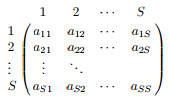
\includegraphics[scale = 0.67]{ma.PNG}\hspace{50mm}  
\end{center} 
\end{figure}
Donde $a_{ij}$ corresponde a la probabilidad de que la persona $t + 1$ hago un pago $j$ dado que la persona $t$ hizo un pago $i$.
\\
\\
\textrm{\large Entrada}
\\
Un entero $C$, $1 ≤ C ≤ 100$, que es el número de casos a procesar seguido de una línea en blanco. Por cada caso de entrada, se recibirán dos enteros $5 ≤ N ≤ 500$ , $3 ≤ S ≤ 15$ y a continuación $N$ observaciones dónde apareceran los tipos de pagos $X = {1, 2, . . . , S}$.
\\
\\
\textrm{\large Salida}
\\
Deberán aparecer $C$ matrices de transición una por cada caso de la entrada, donde los elementos deberán estar redondeados a dos lugares decimales. Habrá una linea en blanco después de cada matriz.
\\
\\
\textrm{\large Entrada Ejemplo}
\\
2\\
8 4\\
1 2 3 1 1 3 2 4\\
5 3\\
1 2 3 3 1\\
\\
\\
\textrm{\large Salida Ejemplo}
\\
0.33 0.33 0.33 0.00\\
0.00 0.00 0.50 0.50\\
0.50 0.50 0.00 0.00\\
0.00 0.00 0.00 0.00\\
0.00 1.00 0.00\\
0.00 0.00 1.00\\
0.50 0.00 0.50\\
\\
\textrm{\large Entendiendo el problema}\\
Dada una serie de $N$ observaciones y a lo más $S$ tipos de pago, se quiere encontrar una matriz de transiciones entre estos estados. Éstas son las probabilidades de cada estado por cada entrada de la matriz. Esta matriz no es simétrica.
\\
\textrm{\large Solución}\\
Se recorre la cadena de observaciones, se identifica el tipo de observación $o_i$ y $o_{i-1}$, y en una matriz se cuentan dichas incidencias, esta incidencia debe ser del tipo $s= o_{i-1} \rightarrow s' = o_{i}$. Entonces por cada una de estas incidencias podemos hacer \texttt{mat[s][s']++}. Al final cada renglón de la matriz se normaliza por el total de observaciones del tipo $s$.
\\
\textrm{\large Código}\\
\begin{minted}[breaklines,fontsize=\footnotesize,linenos]{java}
import java.util.*;

class Bmain
{
	public static void main(String[] args)
	{
		Scanner sc = new Scanner(System.in);
		int tt = sc.nextInt();
		 
		while (tt-- > 0)
		{
			double mat[][] = new double[20][20], tot[] = new double[20];
			int arr[] = new int[505];
			int S, N;

			N = sc.nextInt();
			S = sc.nextInt();

			for(int j = 0; j < N; j++)
			{
				arr[j] = sc.nextInt();
				arr[j]--;
			}

			for(int j = 0; j < N-1; j++)
			{
				tot[arr[j]]++;
				mat[arr[j]][arr[j+1]]++;
			}

			for(int i = 0; i < S; i++)
			{
				for(int j = 0; j < S; j++)
				{
					if(tot[i] > 0)
						System.out.printf("%.2f ", mat[i][j] / tot[i]);
					else
						System.out.printf("%.2f ", mat[i][j]);
				}
				System.out.println();
			}
			System.out.println();
		}
	}
}
\end{minted}
\newpage
%\hspace{1 cm}--- Linus
\hspace{5 cm}---\textrm{\large C - Contando nombres\footnote[1]{David Felipe Castillo Velázquez - Grupo de Algoritmia Avanzada y Programación Competitiva}}\\
\\
\hspace{10 cm}---\textrm{\raggedright\normalsize  Límite de tiempo: 1 segundo}\\
\\

\hfill
\begin{tabular}{@{}l@{}}
\textbf{Dificultad:} $\star \star \star$ \\
\textbf{Temas:} Matemáticas \\
\textbf{Complejidad:} $O(n^2)$
\end{tabular}\\
\\
Kenny es un ser polinominal, es decir, se le conoce por varios nombres, e.g, “Kenny”, “Kevin”, “Kenan”. Queremos creer que a Kenny no le molesta tener varios nombres, pero al parecer a su novia sí; “¡Se llama Kenny!”, grita cada vez que alguien lo llama con otro nombre. \\ \\Para intentar reducir su enojo, decidimos utilizar nombres que contengan las mismas letras que “Kenny”, i.e, anagramas. Después de un tiempo nos dimos cuenta que ahora
teníamos nombres de sobra para Kenny, y nos dió curiosidad saber exáctamente cuántos. ¿Y por qué detenernos sólo con “Kenny”?
\\
\\
\textrm{\large Entrada}
\\
La primer línea contendrá $t$, $1 ≤ t ≤ 100$, el número de casos de prueba. Para cada caso de prueba, en una línea, habrá una cadena $S$, compuesta por puras letras minúsculas, $1 ≤ longitud(S) ≤ 200$.
\\
\\
\textrm{\large Salida}
\\
Para cada caso de prueba tendrás que imprimir un entero $k mod 10^9 + 7 (1000000007)$, que indica el número de anagramas distintos que existen para la cadena $S$.
\\
\\
\textrm{\large Entrada Ejemplo}
\\
3\\
kenny\\
algoritmia\\
aaaa\\
\\
\\
\textrm{\large Salida Ejemplo}
\\
60\\
907200\\
1\\
\\
\textrm{\large Entendiendo el problema}\\
Dada una cadena de tamaño $n$, compuesta por letras minúsculas, se te pide saber cuántas cadenas diferentes puedes formar usando los caracteres de la cadena.\\
\\
\textrm{\large Solución}\\
Sabemos que podemos acomodar los $n$ caracteres de la cadena en $n!$ formas, creando este número de cadenas. Sin embargo existen algunas cadenas que se repiten, en especial, si $a_i$ es la cantidad que se repite el $i$-ésimo tipo de caracter de la cadena, entonces se repiten $a_1!a_2!...a_k!$ cadenas. Por lo tanto la respuesta es $\displaystyle \frac{n!}{a_1!a_2!...a_k!} = \displaystyle \binom{n}{a_1}\binom{n-a_1}{a_2}...\binom{n-a_1-...-a_{k-1}}{a_k}$\\
\\
\textrm{\large Código}\\
\begin{minted}[breaklines,fontsize=\footnotesize,linenos]{cpp}
#include <bits/stdc++.h>
 
#define For(i, a, b) for(int i=a; i<b; ++i)
#define INF (1<<30)
#define MP make_pair
#define MOD 1000000007
 
using namespace std;
 
typedef pair <int, int> ii;
typedef long long ll;
 
int C[205][205], v[30];
 
int main()
{
    //std::ios_base::sync_with_stdio(false);
 
    For(i, 0, 201)
        For(j, 0, i+1)
            C[i][j] = i == j or j == 0 ? 1 : (C[i-1][j] + C[i-1][j-1]) % MOD;
 
    int tt;
    scanf("%d", &tt);
 
    while (tt--)
    {
        memset(v, 0, sizeof v);
         
        char s[205];
        scanf("%s", s);
 
        int n = strlen(s);
        For(i, 0, n)
            v[s[i]-'a']++;
 
        int ans = 1;
        For(i, 0, 'z'-'a'+1)
        {
            if (v[i] > 0)
                ans = (ans*C[n][v[i]]) % MOD;
            n -= v[i];
        }
 
        printf("%d\n", ans);
    }
 
    return 0;
}
\end{minted}
\newpage
%\hspace{1 cm}--- Linus
\hspace{5 cm}---\textrm{\large D - Dados\footnote[1]{David Felipe Castillo Velázquez - Grupo de Algoritmia Avanzada y Programación Competitiva}}\\
\\
\hspace{10 cm}---\textrm{\raggedright\normalsize  Límite de tiempo: 1 segundo}\\
\\

\hfill
\begin{tabular}{@{}l@{}}
\textbf{Dificultad:} $\star \star$ \\
\textbf{Temas:} Matemáticas \\
\textbf{Complejidad:} $O(1)$
\end{tabular}\\
\\
Seguramente has visto la serie “The Big Bang Theory”, y seguramente has visto el episodio donde Sheldon se basa en unos dados para tomar todas sus decisiones. Cada vez que Sheldon tenía que tomar una decisión lanzaba los dados y le asignaba a cada opción un número, dependiendo de la suma de los dados, elegía la opción asociada.\\
\\Nosotros queremos adoptar la estrategia de Sheldon, sin embargo hay momentos en que definitivamente tenemos preferencia por una opción, por ejemplo, cuando decidimos entre <hacer la tarea> o <programar>, preferimos que salga la segunda.\\
\\De acuerdo a la cantidad de dados que usamos para decidir y el número de caras que tienen los dados, queremos que nos ayudes a saber qué número asociarle a nuestra opción preferida para tener la mayor probabilidad de elegirla.
\\
\\
\textrm{\large Entrada}
\\
La primer línea contendrá el número de casos de prueba $t$, $1 ≤ t ≤ 100$. Para cada caso de prueba, en una línea, habrá dos enteros $n$ y $m$, $1 ≤ n, m ≤ 50$, el número de dados que usamos y el número de caras de los dados, respectivamente. Las caras de los dados están marcadas del $1$ al $m$.
\\
\\
\textrm{\large Salida}
\\
Para cada caso de prueba tendrás que imprimir la suma de los dados que tiene la mayor probabilidad de salir, si existen varias soluciones, imprime la menor de ellas.
\\
\\
\textrm{\large Entrada Ejemplo}
\\
3\\
1 6\\
2 6\\
50 50\\
\\
\\
\textrm{\large Salida Ejemplo}
\\
1\\
7\\
1275\\
\\
\textrm{\large Entendiendo el problema}\\
Dados $n$ dados, todos con $m$ caras, quieres saber cuál es la suma de las caras de los dados con mayor probabilidad de salir al lanzar todos los dados.
\\
\textrm{\large Solución}\\
Sea $a$ y $b$ el mínimo y máximo, respecticamente, valor posible para la suma. Entonces es fácil ver que la respuesta es $\displaystyle \frac{a+b}{2}$.
\\
\textrm{\large Código}\\
\begin{minted}[breaklines,fontsize=\footnotesize,linenos]{cpp}
#include <bits/stdc++.h>
 
#define For(i, a, b) for(int i=(a); i<(b); ++i)
#define INF 1000000000
#define MP make_pair
 
using namespace std;
 
typedef pair <int, int> ii;
typedef long long ll;
 
double p[55][2505];
 
int main()
{
    //std::ios_base::sync_with_stdio(false);
     
    int tt;
    scanf("%d", &tt);
 
    while (tt--)
    {
        int n, m;
        scanf("%d %d", &n, &m);
        printf("%d\n", n == 1 ? 1 : (n*m - n)/2 + n);
    }
 
    return 0;
}
\end{minted}
\newpage
%\hspace{1 cm}--- Linus
\hspace{5 cm}---\textrm{\large E - Encriptando Mensajes\footnote[1]{Kenny Yahir Méndez Ramírez - Grupo de Algoritmia Avanzada y Programación Competitiva}}\\
\\
\hspace{10 cm}---\textrm{\raggedright\normalsize  Límite de tiempo: 1 segundo}\\

\hfill
\begin{tabular}{@{}l@{}}
\textbf{Dificultad:} $\star$ \\
\textbf{Temas:} Implementación \\
\textbf{Complejidad:} $O(n)$
\end{tabular}
\\
\\
David es un chico singular, muy discreto, no le gustan las imprudencias. Por tanto es de esperarse que sus actividades las realice de manera muy reservada. Tanto así que en estos últimos dias se le ha ocurrido la idea de encriptar sus mensajes que manda por Face a sus amigos. Una manera muy fácil de hacerlo, y muy conocida además, es utilizar la operación binaria XOR, esta es, dados dos enteros x y k donde al ´ultimo lo usamos como clave, obtenemos un entero $y = x XOR k$ que puede ser usado para devolvernos el valor de $x$ ejecutando la operación $y XOR k$. Sabiendo esto, nos percatamos que con reconocer el valor de la clave $k$ podemos enviar cualquier mensaje entre todos los que conozcan tal valor.\\ \\Bien, como tú formas parte del circulo social de David deberáss crear tu
propio programa que encripte los mensajes que quieras enviarle, proporcion´andote la clave que David ha elegido para ti.
\\
\\
\textrm{\large Entrada}
\\
La primera línea contendrá un entero $C$ que son los casos a procesar. En los siguientes $C$ bloques aparecer´´4 un un entero $1 ≤ k ≤ 31$ en la primera linea y en la segunda linea el mensaje a encriptar. La linea no usar más 1000 caracteres.
\\
\\
\textrm{\large Salida}
\\
Serán $C$ lineas, en cada una el mensaje encriptado para cada clave correspondiente.
\\
\\
\textrm{\large Entrada Ejemplo}
\\
2\\
5\\
Hola, que tal estas?\\
31\\
\\
\\
\textrm{\large Salida Ejemplo}
\\
Mjid)\%tp‘\%qdi\%‘vqdv:\\
Pfz3?zs?ji~?zlk~?|~v{p?izm{~{\\
\\
\textrm{\large Entendiendo el problema}\\
Dada una cadena $s$ y un entero $k$, se te pide que encriptes $s$ haciendo $x$ XOR $k$ para cada caracter $x$ de $s$.\\
\\
\textrm{\large Solución}\\
Directa.\\
\\
\textrm{\large Código}\\
\begin{minted}[breaklines,fontsize=\footnotesize,linenos]{cpp}
#include <cstdio>
#include <iostream>
#include <string>
#define For(x,a,b) for(int x=(a); x<(b); x++)
using namespace std;
 
int main()
{
    int C,k;
    string cad;
 
    scanf("%d",&C);
 
    For(c,0,C)
    {
        cin >> k;
        getline(cin,cad);
        getline(cin,cad);
 
        For(i,0,cad.size())
        {
            printf("%c ",(cad[i]^k));
        }
        printf("\n");
    }
    return 0;
}
\end{minted}
\newpage
%\hspace{1 cm}--- Linus
\hspace{5 cm}---\textrm{\large F - Focos\footnote[1]{David Felipe Castillo Velázquez - Grupo de Algoritmia Avanzada y Programación Competitiva}}\\
\\
\hspace{10 cm}---\textrm{\raggedright\normalsize  Límite de tiempo: 1 segundo}\\
\\

\hfill
\begin{tabular}{@{}l@{}}
\textbf{Dificultad:} $\star \star$ \\
\textbf{Temas:} Matemáticas \\
\textbf{Complejidad:} $O(1)$
\end{tabular}\\
\\
El interruptor de la luz del cubo de Algoritmia se descompuso, pero afortunadamente, en el CEDETEC, hay un interruptor universal que cambia de estado, de forma un poco peculiar, los focos de todos los cubos. Después de un rato jugando con el interruptor descubrimos que en la i-ésima vez que accionamos el interruptor, los focos de los cubos cuya numeración es divisible por i, cambian de estado; si están apagados se prenden y si están prendidos
se apagan. Por ejemplo, si es la segunda vez que accionamos el interruptor, los focos de los cubos $2, 4, 6, 8, ...$ cambian de estado. El número del cubo de algoritmia es n y suponemos que después de n veces que accionemos el interruptor, el cubo va a tener luz. Ayúdanos a comprobar si ´esto es cierto. El foco del cubo est´a inicialmente
apagado.
\\
\\
\textrm{\large Entrada}
\\
La primer línea contendrá el número de casos de prueba $t, 1 ≤ t ≤ 100$. Para cada caso de prueba, en una línea, habrpa un entero $n, 1 ≤ n ≤ 1018$, descrito anteriormente.
\\
\\
\textrm{\large Salida}
\\
Para cada caso de prueba tendrás que imprimir la cadena “les hace falta estudiar” si es que el foco del cubo de algoritmia termina apagado, o “son unos genios” en caso contrario.
\\
\\
\textrm{\large Entrada Ejemplo}
\\
3\\
7\\
1\\
16\\
S\\
\\
\textrm{\large Salida Ejemplo}
\\
les hace falta estudiar\\
son unos genios\\
son unos genios\\
\\
\textrm{\large Entendiendo el problema}\\
Se te da un arreglo de focos y un interruptor que, al accionarlo la $i$-ésima vez, cambia el estado de los focos que son múltiplos de $i$. Después de accionar $n$ veces el interruptor, quieres saber el estado del $n$-ésimo foco, el cuál está inicialmente apagado.
\\
\textrm{\large Solución}\\
Si el número de divisores de $n$ es par, el foco estará apagado, sino estará prendido. Un entero $n$ tiene un número par de divisores si y sólo si es un cuadrado perfecto.
\\
\textrm{\large Código}\\
\begin{minted}[breaklines,fontsize=\footnotesize,linenos]{cpp}
#include <bits/stdc++.h>
 
#define For(i, a, b) for(int i=a; i<b; ++i)
#define INF (1<<30)
#define MP make_pair
 
using namespace std;
 
typedef pair <int, int> ii;
typedef long long ll;
 
int main()
{
    //std::ios_base::sync_with_stdio(false);
 
    int tt;
    scanf("%d", &tt);
 
    while (tt--)
    {
        int n;
        scanf("%d", &n);
 
        int r = sqrt(n);
        printf("%s\n", r*r == n ? "son unos genios" : "les hace falta estudiar");
    }
 
    return 0;
}
\end{minted}
\newpage
%\hspace{1 cm}--- Linus
\hspace{5 cm}---\textrm{\large G - Grupos\footnote[1]{David Felipe Castillo Velázquez - Grupo de Algoritmia Avanzada y Programación Competitiva}}\\
\\
\hspace{10 cm}---\textrm{\raggedright\normalsize  Límite de tiempo: 1 segundo}\\
\\

\hfill
\begin{tabular}{@{}l@{}}
\textbf{Dificultad:} $\star$ \\
\textbf{Temas:} Ad-hoc \\
\textbf{Complejidad:} $O(nm)$
\end{tabular}\\
\\
La coordinación de MAC necesita asignarle los grupos a los alumnos de nuevo ingreso, sin embargo no quieren asignarlos completamente de forma aleatoria. Ellos quieren evitar que en un grupo haya dos o más personas con exactamente la misma personalidad, pues de ser así, esos alumnos podrían causar muchos problemas.\\
\\Se te ha pedido que ayudes a verificar si es posible realizar una asignación de los alumnos que cumpla los requerimientos de la coordinación, dados el número de alumnos, la personalidad de cada uno de ellos y el número de alumnos que debe tener cada grupo.\\
\\La personalidad de un alumno estará representada por un entero $a_i$. Todos los grupos deben tener la misma cantidad de alumnos.
\\
\\
\textrm{\large Entrada}
\\
La primera línea contiene un entero $t, 1 ≤ t ≤ 100$, el número de casos de prueba. Para cada caso de prueba habrá dos líneas. La primera contendrá dos enteros $n$ y $m$, $1 ≤ n, m ≤ 100$, el número de grupos y el número de alumnos que debe tener cada grupo, respectivamente. La segunda línea tendá $nm$ enteros $a_i$ ,$ 0 ≤ ai ≤ 105$ ,
separados por espacio, que representan la personalidad del alumno i.
\\
\\
\textrm{\large Salida}
\\
Para cada caso de prueba debes imprimir, en una línea, la cadena “si”, si es posible asignar los alumnos de tal forma que no existan dos o más alumnos con la misma personalidad en el mismo grupo. De no existir una asignación, imprime la cadena “no”.
\\
\\
\textrm{\large Entrada Ejemplo}
\\
3\\
4 4\\
5 5 2 3 3 4 8 7 2 5 1 5 2 4 3 2\\
1 1\\
5\\
2 3\\
1 1 1 1 1 1\\
\\
\\
\textrm{\large Salida Ejemplo}
\\
si\\
si\\
no\\
\\
\textrm{\large Entendiendo el problema}\\
Dados $n$ grupos, donde deben haber $m$ alumnos, $nm$ alumnos y la personalidad $a_i$ del $i$-ésimo alumno, quieres saber si es posible asignar los alumnos a los grupos de tal forma que no haya un grupo con más de un alumno de la misma personalidad.
\\
\textrm{\large Solución}\\
Si existen $k > n$ alumnos con la misma personalidad, es imposible crear los grupos, en caso contrario es siempre posible.\\
\\
\textrm{\large Código}\\
\begin{minted}[breaklines,fontsize=\footnotesize,linenos]{cpp}
#include <bits/stdc++.h>
 
#define For(i, a, b) for(int i=a; i<b; ++i)
#define INF (1<<30)
#define MP make_pair
 
using namespace std;
 
typedef pair <int, int> ii;
typedef long long ll;
 
int a[100005];
 
int main()
{
    //std::ios_base::sync_with_stdio(false);
 
    int tt;
    scanf("%d", &tt);
 
    while (tt--)
    {
        memset(a, 0, sizeof a);
 
        int n, m;
        scanf("%d %d", &n, &m);
 
        bool ok = true;
        For(i, 0, n*m)
        {
            int x;
            scanf("%d", &x);
            a[x]++;
            if (a[x] > n)
                ok = false;
        }
 
        printf("%s\n", ok ? "si" : "no");
    }
 
    return 0;
}
\end{minted}
\newpage
\section{concurso de programación}{\large XIV Semana de MAC}\\

%\hspace{1 cm}--- Linus
\hspace{5 cm}---\textrm{\large A - Armando Elecciones\footnote[1]{Silverio Flores Moroni - Grupo de Algoritmia Avanzada y Programación Competitiva}}\\
\\
\hspace{10 cm}---\textrm{\raggedright\normalsize  Límite de tiempo: 5 segundos}\\
\\

\hfill
\begin{tabular}{@{}l@{}}
\textbf{Dificultad:} $\star\star\star$ \\
\textbf{Temas:} Teoría de Gráficas \\
Busquedas \\
\textbf{Complejidad:} $O(n+r)$
\end{tabular}\\
\\
En Maclandia se llevarán a cabo elecciones presidenciales muy pronto, pero dado que conllevan un costo muy elevado, su Instituto Electoral te ha encargado que les digas si es posible determinar quién ganará las elecciones presidenciales, ya que si esto es posible, les ahorrarías mucho dinero.\\
\\En Maclandia ocurren muchas situaciones que no ocurren en los demás paises de su planeta Namek, por ejemplo: debido a ciertas influencias (dinero, dinero, dinero, nepotismo, etc.), el voto de algunas personas vale más que el de otras; además, si una persona vota por cierto candidato todos sus amigos votarán por el mismo candidato; aquellas personas que no tengan amigos con un voto definido, el día de las elecciones votarán por algún candidato según su sano juicio.\\
\\Las personas en Maclandia tienen agregados a todos sus amigos en su red social, y si una persona es amiga de otra, entonces esta otra también es amiga de esa persona. Es bien sabido que los candidatos votarán por ellos mismos.\\
\\Sin embargo en este país existen dos genios: uno malvado y uno bueno. Si alguien es amigo del genio malvado entonces el candidato por el que votaría perderá las elecciones, sin importar el valor de los votos que haya obtenido.\\
\\En caso contrario si alguien es amigo del genio bueno, el candidato por el que votaría ganará las elecciones. Si los genios intentan hacer que el mismo candidato gane y pierda las elecciones entonces se anularán sus poderes y no tendrán poder sobre las elecciones. Si algún genio no tiene amigos, entonces este no podrá ejercer su poder para influir en las elecciones. Los genios sólo pueden ser amigos (directa o indirectamente) de personas que ya tienen predeterminado su voto. Ninguna persona votará por dos candidatos, puesto que ninguna persona será amiga indirecta de dos candidatos al mismo tiempo. Un genio es considerado como una persona en sus relaciones de amistad.\\
\\
\textrm{\large Entrada}
\\
La primera línea será un entero $1 ≤ T ≤ 100$, indicando la cantidad de casos de prueba. Cada caso de prueba se compondrá de varias lineas: la primera tendrá tres números $n$, $c$ y $r$ $(2 ≤ n ≤ c ≤ 500, 0 ≤ r ≤ (n + 2 − c)2)$ indicando el número de votantes, el número de candidatos y el número de relaciones de amistad respectivamente.\\
\\Los votantes son identificados con los números 1 hasta $n$ inclusive. La siguiente línea tendrá $n$ números enteros $(1 ≤ a_j ≤ 10000)$ , el j-ésimo número indicará la cantidad de puntos que vale el voto de la j-ésima persona. En la siguiente línea vendrán $c$ números, los cuales indican el número de cada candidato. $r$ líneas vendrán después, cada una con dos números $−1 ≤ a, b ≤ n$, indicando que las personas $a$ y $b$ son amigas. La persona 0 es el genio bueno, y la persona $−1$ es el genio malvado. Los casos de prueba están separados por una línea en blanco.
\\
\\
\textrm{\large Salida}
\\
Para cada caso, indica en una línea distinta: el número del candidato que ganará las elecciones, si es posible determinar quien las ganara; si no es posible determinar esto, imprime “Es mas facil salir de la friendzone que saber quien ganara” sin las comillas.
\\
\\
\textrm{\large Entrada Ejemplo}
\\
2\\
4 3 3\\
1 10 30 1\\
1 2 3\\
1 4\\
2 0\\
3 -1\\
5 3 2\\
1 50 10 2 20\\
1 2 3\\
1 4\\
2 -1\\
\\
\\
\textrm{\large Salida Ejemplo}
\\
2\\
Es mas facil salir de la friendzone que saber quien ganara\\
\\Explicación de la entrada ejemplo\\
\\En el segundo caso, la persona 2 pierde las elecciones automaticamente porque es amiga del genio malvado, la persona 1 puede juntar 3 puntos resultado de la suma de sus puntos y los de sus amistades, la persona 3 puede juntar 10 puntos. Sin embargo no es posible determinar quien ganará la elección, a pesar de que la persona 3 tiene
más puntos, porque la persona 5, que no es amiga directa/indirecta de algún candidato, cuando vote puede hacerlo por alguno de los dos (1 ó 3) inclinando la balanza a favor de cualquiera.\\
\\
\textrm{\large Entendiendo el problema}\\
Para cada caso de prueba se debe construir una gráfica con las relaciones de amistad como aristas y como vértices las $n$ personas. Cada candidato representa una componente de la gráfica. \\
\\
\textrm{\large Solución}\\
Para cada candidato se realiza una búsqueda en amplitud y por cada vértice que puede alcanzar se suma la cantidad de puntos que ese vértice tiene. Se considera que el genio malo aporta $-\infty$ puntos y el bueno $\infty$. Al final se suman los puntos de aquellas personas que no pertecen a ninguna componente representada por algun candidato; si esta suma más los puntos del segundo candidato más alto (en puntos) es mayor o igual a los puntos del candidato más alto entonces no es posible determinar quién ganará las eleciones, en caso contrario las gana el candidato con más puntos.\\
\\
\textrm{\large Código}\\
\begin{minted}[breaklines,fontsize=\footnotesize,linenos]{cpp}
#include <iostream>
#include <queue>
#include <algorithm>
using namespace std;
 
queue <int> cola;
int matriz[505][505], votos[505], personas[505];
pair <int, int> candidatos[505];
int infinito=100000000;
int n;
 
int buscar()
{
    int suma =0, a, i;
    bool ganaste=false, perdiste=false;
    while (!cola.empty() )
    {
        a=cola.front();
        cola.pop();
        if ( personas[a] ) continue;
 
        if (a==0)   ganaste=true;
        else if (a==n+1) perdiste=true;
        else suma += votos[a];
        personas[a]=1;
        for (i=-1; ++i<=n+1; )
            if (matriz[a][i]==1)
                cola.push(i);
    }
    if (ganaste && !perdiste) suma= infinito;
    if (perdiste && !ganaste) suma =-infinito;
    return suma;
}
 
int main()
{
    int t, c, r, a, b, i, j;
    cin>>t;
    while (t--)
    {
        cin>>n>>c>>r;
 
        //limpiar
        while (!cola.empty() ) cola.pop();
        for (i=-1; ++i<=n+1; )
            for (j=-1; ++j<=n+1; )
                matriz[i][j]=0;
        for (i=-1; ++i<=n+1; )
            personas[i]=0;
        for (i=-1; ++i<c; )
            candidatos[i].first=0;
        votos[0]=votos[n+1]=0;
 
        for (i=0; ++i<=n; )
            cin>>votos[i];
 
        for (i=-1; ++i<c; )
            cin>>candidatos[i].second;
 
        while (r--)
        {
            cin>>a>>b;
            if (a==-1) a=n+1;
            if (b==-1) b=n+1;
            matriz[a][b]=1;
            matriz[b][a]=1;
        }
 
        for (i=-1; ++i<c; )
        {
            cola.push( candidatos[i].second );
            candidatos[i].first = buscar();
        }
 
        sort(candidatos, candidatos+c);
 
        if (candidatos[c-1].first==infinito  || candidatos[c-2].first==-infinito )
            cout<<candidatos[c-1].second<<endl;
        else
        {
            //contar los no amigos
            int otrasuma=0;
            for (i=0; ++i<=n; )
                if ( personas[i]==0 )
                    otrasuma+=votos[i];
            if ( (candidatos[c-2].first + otrasuma) >= candidatos[c-1].first )
                cout<<"Es mas facil salir de la friendzone que saber quien ganara\n";
            else
                cout<<candidatos[c-1].second<<"'\n";
        }
    }
    return 0;
}
\end{minted}
\newpage
%\hspace{1 cm}--- Linus
\hspace{5 cm}---\textrm{\large B - Buscando amigos\footnote[1]{Silverio Flores Moroni - Grupo de Algoritmia Avanzada y Programación Competitiva}}\\
\\
\hspace{10 cm}---\textrm{\raggedright\normalsize  Límite de tiempo: 3 segundos}\\
\\

\hfill
\begin{tabular}{@{}l@{}}
\textbf{Dificultad:} $\star\star\star$ \\
\textbf{Temas:} Matemáticas \\
Teoría de Números \\
\textbf{Complejidad:} $O(n)$
\end{tabular}\\
\\
Después de una intensa jornada de actividades en la semana de MAC, algunos alumnos han encontrado a quien consideran “el amor de su vida”. Sin embargo muchos estudiantes de MAC se consideran a sí mismos matemáticos puros y no le hablan a cualquier persona. Los alumnos que se inscribieron a la semana de MAC recibieron un id (numero de identificación) para poder entrar a las conferencias. Los matemáticos puros sólo le hablarán a la persona cuyo id $a$ sea amigo de su id $b$. Un número a es amigo de b si la suma de los divisores de a (exceptuando sólo a a) es igual a b, nota que si a es amigo de b, b no necesariamente es amigo de a. Algunos alumnos de MAC han recurrido a ti debido a tus grandes conocimientos en estas áreas del saber para saber si “el amor de su vida” les hablará. Por causas fortuitas todos estos amores son matemáticos puros. Tu tarea es determinar si los alumnos tienen oportunidad de hablar con quienes consideran el amor de su vida.
\\
\\
\textrm{\large Entrada}
\\
La primer lpinea de la entrada contendrá un entero $T ≤ 200$, el número de casos de prueba, a continuación se darán $T$ renglones, cada uno con un caso de prueba. Cada renglón tendrá dos números a, b, tales que $1 ≤ a, b ≤ 10000$
\\
\\
\textrm{\large Salida}
\\
Para cada caso de prueba imprime “Quiza y sin quiza”, sin las comillas si a es amigo de b; imprime “Llora desconsoladamente” en caso contrario.
\\
\\
\textrm{\large Entrada Ejemplo}
\\
3\\
6 5\\
3 10\\
1184 1210\\
\\
\\
\textrm{\large Salida Ejemplo}
\\
Llora desconsoladamente\\
Llora desconsoladamente\\
Quiza y sin quiza\\
\\
\textrm{\large Entendiendo el problema}\\
Debemos saber si la suma de los divisores propios de un número $a$ son iguales a un número $b$. 
\\
\textrm{\large Solución}\\
En este concuso se permitió la solucion ``naive'', la cual consisitia en verificar todos los números menores a $a$ y sumar aquellos que lo dividen, después verificar si esa suma es igual a $b$. Sin embargo existe una mejor solucion:

Sean $p_1, p_2, \ldots, p_k$ los factores primos de $a$. Podemos decir que: 
$$a=p_1^{f_1} \times p_2^{f_2} \times \ldots \times p_k^{f_k} $$
La suma de los divisores de $a$, incluyendo a $a$ es:
$$S=\frac{p_1^{f_1+1}-1}{p_1-1} \times \frac{p_2^{f_2+1}-1}{p_2-1} \times \ldots \times \frac{p_k^{f_k+1}-1}{p_k-1} $$
Entonces basta con verificar si $S-a=b$. A pesar de que esta solución se ve mas compleja, computacionalmente es mejor y más rápida.\\
\\
\textrm{\large Código}\\
\begin{minted}[breaklines,fontsize=\footnotesize,linenos]{cpp}
#include <iostream>
using namespace std;
int factores[1000][2], i;
 
void descomponer(int a)
{
    int j =1;
    while (a!=1)
    {
        ++j;
        if (a%j==0)
        {
            ++i;
            factores[i][0]=j;
            while (a%j==0)
            {
                ++factores[i][1];
                a /=j ;
            }
        }
    }
}
 
int geometrica(int j)
{
    int k, res=1;
    for (k=-1; ++k<=factores[j][1]; )
        res *=factores[j][0];
    --res;
    res /=(factores[j][0]-1);
    return res;
}
 
int main()
{
    int t, a, b, j,m, res;
    cin>>t;
    while (t--)
    {
        cin>>a>>b;
        i=-1;
 
        for (j=-1; ++j<1000; factores[j][1]=0);  //limpiar
 
        descomponer(a);
 
        res=1;
        for (j=-1; ++j<=i;)
        {
            res *=geometrica(j);
        }
        res -=a;
        if (res!=b)
            cout<<"Llora desconsoladamente\n";
        else cout<<"Quiza y sin quiza\n";
    }
}
\end{minted}
\newpage
%\hspace{1 cm}--- Linus
\hspace{5 cm}---\textrm{\large C - Caballo sin mecate\footnote[1]{Édgar García Rodríguez - Grupo de Algoritmia Avanzada y Programación Competitiva}}\\
\\
\hspace{10 cm}---\textrm{\raggedright\normalsize  Límite de tiempo: 1 segundo}\\

\hfill
\begin{tabular}{@{}l@{}}
\textbf{Dificultad:} $\star\star$ \\
\textbf{Temas:} Teoría de Grafos \\
Busquedas \\
\textbf{Complejidad:} $O(n+m)$
\end{tabular}
\\
\\
Ultimamente los integrantes del Grupo de Algoritmia se han obsesionado con el milenario juego de ajedrez, pero tienen un inconviente, puesto que Moro siempre les gana, han decidido inventar un nuevo juego al que llamaron “Caballo sin Mecate”.\\
\\El juego consiste en un tablero de ajedrez de tamaño $n × m$ en el que interactúan dos jugadores. Dada una configuración de piezas tienes que llegar en la menor cantidad de pasos con el caballo de un punto a otro del tablero; gana el jugador que pueda dar la menor cantidad de movimientos. Además, se estipula que en el tablero sólo hay un caballo y múltiples piezas de otros tipos de las cuales no puede ocupar su lugar, pero sí saltarlas.\\
\\El caballo no se desplaza en línea recta, sino que tiene un movimiento característico llamado salto. El salto del caballo se parece a una L, y se compone de un desplazamiento de dos casillas en dirección horizontal o vertical, y otra casilla más en ángulo recto (en el diagrama siguiente, los cuadros marcados son los posibles lugares hacia donde puede desplazarse el caballo).
\begin{figure}[h!] 
\begin{center} 
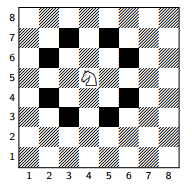
\includegraphics[scale = 1]{cab.PNG}\hspace{50mm}  
\end{center} 
\end{figure}
\\Tu tarea es ayudarnos a encontrar el número mínimo de movimientos que le tomará al caballo llegar a cierto punto, dada una configuración, para así poderle ganar a Moro.
\\
\\
\textrm{\large Entrada}
\\
La primer línea contendra un solo número $T (1 ≤ T ≤ 100)$ que representa la cantidad de casos de prueba, que se seguirá de $T$ casos de prueba. La primer línea de cada caso contendrá dos números enteros $n$ y $m (1 ≤ n, m ≤ 100)$. Seguirán $n$ lineas, una línea por cada fila del tablero, donde cada línea tendrá $m$ caracteres $c_{ij}$ , que representan el estado del $escaque^1$ de la i-ésima fila y la j-ésima columna (numerados de abajo hacia arriba y de izquierda a derecha como se muestra en el diagrama anterior). Donde $c_{ij}$ puede ser una casilla vacía (*), un peón (p) , una torre (t), un alfil (b), un rey (k), una reina (q) o un único caballo (c) para todo el tablero. La última línea de cada caso tendrá dos enteros $x$, y $(1 ≤ x ≤ n, 1 ≤ y ≤ m)$ que representan la fila y columna a las que quieres llegar.
\\
\\
\textrm{\large Salida}
\\
Por cada caso deberás imprimir una sola línea que contendrá un entero que es la cantidad mínima de movimientos del caballo para llegar a su destino o $-1$ en caso de que sea imposible llegar a esa casilla.
\\
\\
\textrm{\large Entrada Ejemplo}
\\
2\\
7 8\\
********\\
********\\
********\\
********\\
********\\
bbbqkptt\\
*c******\\
1 6\\
2 2\\
**\\
c*\\
2 2\\
\\
\\
\textrm{\large Salida Ejemplo}
\\
4\\
-1\\
\\Notas
\\En el primer caso se puede llegar de la siguiente manera:
\begin{figure}[h!] 
\begin{center} 
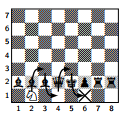
\includegraphics[scale = .6]{cab1.PNG}\hspace{50mm}  
\end{center} 
\end{figure}
\\En el segundo caso no hay manera de llegar a la casilla
(2, 2).
\\
\textrm{\large Entendiendo el problema}\\
Debemos determinar el mínimo número de movimientos requeridos para que el caballo llegue a cierta pocisión del tablero, si es que ésto es posible.
\\
\textrm{\large Solución}\\
El grafo es implícito y es el tablero de ajedrez, y decimos que un vértice (escaque) es vecino de otro si se puede llegar de uno a otro por medio de un movimiento de caballo, los vértices que tienen una pieza de ajedrez, que no es el caballo, en ellos no tienen vecinos.
Para resolver el problema realizamos una búsqueda en amplitud desde la posición inicial del caballo contando los movimientos requeridos para llegar a cierto lugar, si en la búsqueda no se encuentra la posción deseada decimos que es imposible.
\\
\textrm{\large Código}\\
\begin{minted}[breaklines,fontsize=\footnotesize,linenos]{java}
import java.util.*;
 
class Cmain
{
    static class pair
    {
        public int x, y;
        public pair(int _x, int _y)
        {
            x = _x;
            y = _y;
        }
    }
 
    static int dX[] = {-2, -1, 1, 2, 2, 1, -1, -2}, dY[] = {1, 2, 2, 1, -1, -2, -2, -1};
 
    public static void main(String[] args)
    {
        Scanner sc = new Scanner(System.in);
        int tt = sc.nextInt();
 
        while (tt-- > 0)
        {
            int n = sc.nextInt(), m = sc.nextInt();
            String board[] = new String[n];
 
            sc.nextLine();
            for (int i = 0; i < n; ++i)
                board[i] = sc.nextLine();
 
            int xf = sc.nextInt(), yf = sc.nextInt();
            xf = n-xf;
            --yf;
 
            int dist[][] = new int[n][m];
            Queue<pair> cola = new LinkedList<pair>();
 
            for (int i = 0; i < n; ++i)
                for (int j = 0; j < m; ++j)
                    if (board[i].charAt(j) == 'c')
                    {
                        cola.add(new pair(i, j));
                        dist[i][j] = 1;
                    }
 
            while (!cola.isEmpty())
            {
                pair act = cola.remove();
 
                if (act.x == xf && act.y == yf)
                    break;
 
                for (int k = 0; k < 8; ++k)
                {
                    int nx = act.x+dX[k], ny = act.y+dY[k];
 
                    if (nx < 0 || nx >= n || ny < 0 || ny >= m || board[nx].charAt(ny) != '*' || dist[nx][ny] != 0)
                        continue;
 
                    cola.add(new pair(nx, ny));
                    dist[nx][ny] = dist[act.x][act.y] + 1;
                }
            }
 
            System.out.println(dist[xf][yf]-1);
        }
    }
}
\end{minted}
\newpage
%\hspace{1 cm}--- Linus
\hspace{5 cm}---\textrm{\large D - Doncella Jean\footnote[1]{Kenny Yahir Méndez Ramírez - Grupo de Algoritmia Avanzada y Programación Competitiva}}\\
\\
\hspace{10 cm}---\textrm{\raggedright\normalsize  Límite de tiempo: 1 segundo}\\
\\

\begin{figure}[h!] 
\begin{center} 

\includegraphics[scale = 1]{cora.PNG}\hspace{50mm}  
\end{center} 
\end{figure}

\hfill
\begin{tabular}{@{}l@{}}
\textbf{Dificultad:} -$\star$ \\
\textbf{Temas:} Ad Hoc \\
\textbf{Complejidad:} $O(n)$
\end{tabular}
\\
\\En un lejano reino, existe una Doncella llamada Jean, es una chica muy bella pero también muy peculiar. Con lo anterior nos referimos a que tiene costumbres poco casuales. Para resumir, ella cuenta con muchos pretendientes en los reinos vecinos, incluyendo el suyo. Algunos de ellos son príncipes, duques y algunos otros con buen estatus social. No obstante hay un plebeyo que está enamorado de ella, para su fortuna (o no) es un “friend” de nuestra querida doncella, y como se imaginarán ambos tienen una amistad por Facebook.\\
\\Nuestro desdichado plebeyo (llamado Anselmo) últimamente ha tenido charlas muy frecuentes con la Doncella, él siente que varios de los mensajes de ella son indirectas pero no está muy seguro. Para serciorarse de ello ha seleccionado $N$ mensajes y los ha marcado como “Le gusto” y “No le gusto”. El piensa que si la proporción de “Le gusto” es significativamente mayor a la de “No le gusto” entonces decidirá si está en la friendzone o no. Para no complicarse define que si la proporción de “No le gusto” es $≥ 0,2$ entonces se encuentra en la friendzone.\\
\\Ayuda a Anselmo a determinar si se encuentra en la friendzone o no dados los $N$ mensajes de las últimas conversaciones.
\\
\\
\textrm{\large Entrada}
\\
La primer línea es un número $C$ que denota la cantidad de casos de entrada. En los siguientes $C$ bloques aparecerán un número $2 ≤ N ≤ 10000$ y $N$ mensajes. Los mensajes serán “si” y “no” para denotar “Le gusto” y “No le gusto” respectivamente.
\\
\\
\textrm{\large Salida}
\\
Para cada caso deberás imprimir como respuesta “friendzone” cuando $r ≥ 0.2$ donde $r$ denota la proporción de “No le gusto”, en caso contrario la carita feliz “:)”.
\\
\\
\textrm{\large Entrada Ejemplo}
\\
3\\
4\\
si\\
si\\
no\\
si\\
5\\
si\\
si\\
si\\
si\\
si\\
8\\
si\\
no\\
si\\
si\\
si\\
si\\
si\\
si\\
\\
\\
\textrm{\large Salida Ejemplo}
\\
friendzone\\
:)\\
:)\\
\\
\textrm{\large Entendiendo el problema}\\
En este caso, la solución es indirecta, se debe de contar cuantas veces aparece la cadena ya sea ``si'' o ``no'' y determinar su proporción.
\\
\textrm{\large Solución}\\
En el caso en el que la proporción de ``no'' sea $\geq 0{.}2$ se imprime \texttt{friendzone}, en caso contrario \texttt{:)}.
\\
\textrm{\large Código}\\
\begin{minted}[breaklines,fontsize=\footnotesize,linenos]{cpp}
#include <iostream>
#include <cstdio>
#include <cstring>
#include <algorithm>
#include <cmath>
using namespace std;

#define For(x,a,b) for(unsigned int x = (a); x < (unsigned int)(b); x++)

typedef long long ll;


int main()
{
	int C, n, x;
	double r, tol = 0.2;
	string cad;

	scanf("%d",&C);

	while(C--)
	{
		scanf("%d", &n);
		x = 0;
		For(i,0,n){
			cin >> cad;
			x += cad == "no";
		}


		r = (double)x / (double)n;

		if(r < tol)
			printf(":)\n");
		else
			printf("friendzone\n");
	}
	
	return 0;
}
\end{minted}
\newpage
%\hspace{1 cm}--- Linus
\hspace{5 cm}---\textrm{\large E - Explanada\footnote[1]{David Felipe Castillo Velázquez - Grupo de Algoritmia Avanzada y Programación Competitiva}}\\
\\
\hspace{10 cm}---\textrm{\raggedright\normalsize  Límite de tiempo: 1 segundo}\\
\\

\hfill
\begin{tabular}{@{}l@{}}
\textbf{Dificultad:} $\star\star\star \star$ \\
\textbf{Temas:} Matemáticas, Geometría \\
\textbf{Complejidad:} $O(n)$
\end{tabular}\\
\\
Uno de tus amigos ha decido visitarte en la escuela, sin embargo él nunca ha venido a la FES y no sabe cómo encontrarte, por lo tanto has decidido ayudarle para que llegue a la explanada de MAC. La explanada la podemos ver como un polígono $convexo^2$
en el plano, y tú sabes muy bien las coordenadas de todos sus vértices, pues fue lo
primero que te enseñaron en PIMAC. Para poder darle indicaciones a tu amigo necesitas saber si ya ha llegado a la explanada, así que le has pedido que te mande sus coordenadas. Ahora sólo necesitas hacer un programa que te diga si tu amigo está \\
\\
\textrm{\large Entrada}
\\
La primera línea contendrá un entero $1 ≤ t ≤ 100$, el número de casos de prueba. La primera línea de cada caso de prueba será un entero $3 ≤ n ≤ 100$ que denota el número de vértices del polígono que representa a la explanada.\\
\\En las siguientes $n$ líneas de cada caso de prueba habrá dos enteros $0 ≤ x_i
, y_i ≤ 100$ representando las coordenadas del i-ésimo vértice del polígono. Los puntos estarán dados en orden de tal forma que forme un polígono convexo (puede ir en el sentido de las manecillas del reloj o en sentido contrario a las manecillas del reloj). La última línea de cada caso de prueba serán dos enteros $0 ≤ x_a, y_a ≤ 100$, las coordenadas de tu amigo. El punto $(x_a, y_a)$ no va a estar nunca sobre el perímetro del polígono.
\\
\\
\textrm{\large Salida}
\\
Para cada caso de prueba deberás imprimir “si” (sin comillas) si tu amigo está dentro de la explanada, o “no” en caso contrario
\\
\\
\textrm{\large Entrada Ejemplo}
\\
2\\
5\\
1 3\\
2 5\\
4 5\\
5 3\\
2 1\\
4 2\\
5\\
1 3\\
2 5\\
4 5\\
5 3\\
2 1\\
3 3\\
\\
\\
\textrm{\large Salida Ejemplo}
\\
no\\
si\\
\\
\textrm{\large Entendiendo el problema}\\
Dado un polígono convexo de $n$ vértices ($p_0, p_1, \dots , p_{n-1}$ en el orden de las manecillas del reloj o inverso), debemos determinar si un punto $a$ se encuentra dentro del polígono.\\
\\
\textrm{\large Solución}\\
Este un problema bien conocido de geometría computacional que se puede resolver con el Counter Clockwise Test.
Sean $\overrightarrow{ap_i}$ y $\overrightarrow{ap_{i+1}}$ dos vectores obtenidos de estos $3$ puntos. EL producto cruz de $\overrightarrow{ap_i} \times \overrightarrow{ap_{i+1}}$ en otro vector que es perpendicular a ambos. Si la magnitud del vector resultante es positiva/cero/negativa, entonces tenemos que $a$ se encuentra a la derecha/es colineal/izquierda, respectivamente. Entonces si se cumple que para todo $i$ el vector resultante $\overrightarrow{ap_i} \times \overrightarrow{ap_{(i+1) \mod n}}$ tiene el mismo signo, quiere decir, que el punto siempre estuvo del mismo lado de las aristas y por lo tanto se encuentra dentro del polígono convexo.\\
\\
\textrm{\large Código}\\
\begin{minted}[breaklines,fontsize=\footnotesize,linenos]{cpp}
#include <bits/stdc++.h>
#define For(i, a, b) for(int i=(a); i<(b); ++i)
#define INF 1000000000
#define MP make_pair
#define x first
#define y second

using namespace std;

typedef long long ll;
typedef pair <int, int> ii;

ii p[105];
bool ccw(ii A, ii B, ii C)
{
	return (B.x-A.x)*(C.y-A.y) - (B.y-A.y)*(C.x-A.x) >= 0;
}

int main()
{
	int tt;
	scanf("%d", &tt);
	while (tt--)
	{
		int n;
		scanf("%d", &n);
		For(i, 0, n)
			scanf("%d %d", &p[i].x, &p[i].y);
		ii f;
		scanf("%d %d", &f.x, &f.y);
		bool sgn = ccw(f, p[0], p[1]), ok = true;
		For(i, 1, n)
			if (ccw(f, p[i], p[(i+1)%n]) != sgn)
			{
				ok = false;
				break;
			}
		printf("%s\n", ok ? "si" : "no");
	}

	return 0;
}
\end{minted}
\newpage
%\hspace{1 cm}--- Linus
\hspace{5 cm}---\textrm{\large F - Fiesta\footnote[1]{Édgar García Rodríguez - Grupo de Algoritmia Avanzada y Programación Competitiva}}\\
\\
\hspace{10 cm}---\textrm{\raggedright\normalsize  Límite de tiempo: 1 segundo}\\
\\

\hfill
\begin{tabular}{@{}l@{}}
\textbf{Dificultad:} $\star\star\star$ \\
\textbf{Temas:} Matemáticas \\
Probabilidad \\
\textbf{Complejidad:} $O(n*m)$
\end{tabular}\\
\\
Después del intenso concurso de programación de la XIV Semana de MAC tu equipo piensa dar una gran fiesta en tu casa para celebrar su aplastante triunfo sobre los demás equipos.\\
\\El problema es que para entonces tu cerebro ya no podrá trabajar muy bien, puesto que lo exprimiste al máximo en el concurso, y necesitas saber cuál es el valor esperado de la cantidad de personas que asistiran a tu fiesta, por lo que desde ahora harás un programa que te ayude en esta tarea.\\
\\Lamentablemente es probable que no todas las persona asistan a tu fiesta, porque algunas no resolvieron muchos problemas y no se sienten de ánimo.\\
\\Se han invitado $n$ personas a tu fiesta y cada persona tiene una probabilidad $p_i (i = 1, 2, . . . , n)$ de asistir, que está dada en función de su desempeño, es decir,
\begin{figure}[h!] 
\begin{center} 
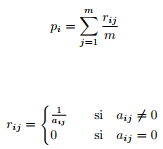
\includegraphics[scale = 1]{form.PNG}\hspace{50mm}  
\end{center} 
\end{figure}
\\donde $a_{ij}$ es igual a la cantidad de intentos que le tomó a la persona $i$ resolver el problema $j$, aij = 0 en caso de
que la i-ésima persona no haya resuelto el j-ésimo problema, $(j = 1, 2, . . . , m)$, y $m$ es la cantidad de problemas en
total .\\
\\
\\
\textrm{\large Entrada}
\\
La primer línea contendra un solo número $T (1 ≤ T ≤ 100)$ que representa la cantidad de casos de prueba.\\
\\La primer línea de cada caso contendrá dos números enteros $n$ y $m (1 ≤ n ≤ 100 , 1 ≤ m ≤ 11)$.\\
\\Seguirán n lineas, una línea por cada persona, donde la i-ésima línea tendrá $m$ enteros $a_{ij} (0 ≤ a_{ij} ≤ 100)$ separados por un espacio.\\
\\
\\
\textrm{\large Salida}
\\
Por cada caso deberás imprimir usa sola línea que contendrá el valor esperado de personas en tu fiesta redondeado a 2 decimales.
\\
\\
\textrm{\large Entrada Ejemplo}
\\
2\\
5 3\\
1 0 1\\
1 1 1\\
0 19 2\\
11 0 2\\
3 0 7\\
4 7\\
1 1 1 1 1 1 1\\
1 1 1 1 1 1 1\\
1 1 1 1 1 1 1\\
1 1 1 1 1 1 1\\
\\
\\
\textrm{\large Salida Ejemplo}
\\
2.21\\
4.00\\
\\Notas
\\En el primer caso la primer persona pudo resolver el primer y tercer problema en un intento, mientras que la segunda resolvió todos, por lo que sus probabilidades de ir son 0,66 y 1 respectivamente.\\
\\En el segundo caso todos resolvieron todos los problemas en un solo intento, por lo que se espera que todos asistan.\\
\\
\textrm{\large Entendiendo el problema}\\
Debemos encontrar el valor esperado del número de personas que asistirán a la fiesta, el cual está dado por la siguiente ecuación:
$$E(X)= \sum_{x=0}^n x f(x)$$
donde $f(x)$ es la probabilidad de que asistan $x$ personas a la fiesta.\\ 
\\
\textrm{\large Solución}\\
Obtner $f(x)$ es algo complicado, ya que para poder obtener esto debemos encontrar todos los subconjuntos $A$ de tamaño $x$ del conjunto $[n]=\{1, 2,\dots, n\}$. Después considerando a $f(x)=1$, decimos que para cada subconjunto $A$, si $i \in A$ entonces $f_A(x)=f_A(x)*p_i$ o en caso contrario $f_A(x)=f_A(x)*(1-p_i)$. Y $f(x)=\sum f_A(x)$
Esta tarea puede sonar bastante complicada, aún así hemos probado que:
\begin{align*} 
E(X) &=  \sum_{i=1}^n p_i \\ 
 &=  \sum_{i=1}^n \sum_{j=1}^m \frac{r_{ij}}{m}\\
 &=\frac{1}{m} \sum_{i=1}^n \sum_{j=1}^m \frac{1}{a_{ij}}
\end{align*}
\\
\textrm{\large Código}\\
\begin{minted}[breaklines,fontsize=\footnotesize,linenos]{cpp}
#include <bits/stdc++.h>
using namespace std;
//look at my code my code is amazing
#define FOR(i, a, b) for (int i = int(a); i < int(b); i++)
#define FOREACH(it, a) for (typeof(a.begin()) it = (a).begin(); it != (a).end(); it++)
#define ROF(i, a, b) for (int i = int(a); i >= int(b); i--)
#define REP(i, a) for (int i = 0; i < int(a); i++)
#define INF 1000000000
#define INFLL 1000000000000000000LL
#define ALL(x) x.begin(), x.end()
#define MP(a, b) make_pair((a), (b))
#define X first
#define Y second
#define EPS 1e-9
#define DEBUG(x)   cerr << #x << ": " << x << " "
#define DEBUGLN(x) cerr << #x << ": " << x << " \n"
typedef pair<int, int> ii;
typedef vector<int> vi;
typedef long long ll;
typedef vector<bool> vb;
//ios_base::sync_with_stdio(0);//fast entrada/salida ;-)
 
void solve()
{
    int n, m;
    scanf("%d %d", &n, &m);
    double ev = 0.0, p = 0.0;
    REP(i, n)
    {
        p = 0.0;
        REP(j, m)
        {
            int a;
            scanf("%d", &a);
            p += (a ? (1.0/a) : 0 );
 
        }
        ev += p/m;
    }
    printf("%.2lf\n", ev);
}
 
int main()
{
    int T;
    scanf("%d", &T);
    REP(i, T)
        solve();
    return 0;
}
\end{minted}
\newpage
%\hspace{1 cm}--- Linus
\hspace{5 cm}---\textrm{\large G - Guiando a Edgar\footnote[1]{David Felipe Castillo Velázquez - Grupo de Algoritmia Avanzada y Programación Competitiva}}\\
\\
\hspace{10 cm}---\textrm{\raggedright\normalsize  Límite de tiempo: 1 segundo}\\
\\

\hfill
\begin{tabular}{@{}l@{}}
\textbf{Dificultad:} $\star\star\star$ \\
\textbf{Temas:} Teoría de Grafos
\textbf{Complejidad:} $O(n^3)$
\end{tabular}\\
\\
Edgar es una persona a la que le gusta optimizar su tiempo, por lo tanto cada que se tiene que desplazar de un lugar a otro dentro de la FES, le gusta irse por el camino que minimice el tiempo que le toma desplazarse. Además
a él le gusta siempre pasar por lugares nuevos, porque asegura que eso ayuda a crear nuevas conexiones neuronales, entonces cada que planea la trayectoria para llegar de un lugar a otro, él considera un camino en específico por el
que debe pasar obligatoriamente.\\
\\En este momento Edgar está demasiado ocupado encargándose del concurso, así que te ha pedido que le ayudes a organizar sus siguientes $Q$ rutas para no tener que perder el tiempo.\\
\\Dado que la FES es muy grande, nos vamos a concentrar sólo en los $N$ lugares favoritos de Edgar, numerados del 1 al N, con caminos entre cada uno de los N lugares. Los caminos entre cada par de lugares i, j, son bidireccionales, es decir, Edgar puede recorrer el camino de i a j o de j a i.
\\
\\
\textrm{\large Entrada}
\\
La primera línea tendra un entero $1 ≤ T ≤ 100$, el número de casos de prueba.\\ La primer línea de cada caso de prueba será un entero $2 ≤ N ≤ 50$, los lugares favoritos en la FES de Edgar, seguido vendrán $N$ líneas, con N enteros cada una. El j-ésimo valor de la i-ésima línea, $1 ≤ w_{ij} ≤ 1000$, indicará el tiempo que le toma a Edgar recorrer el camino del lugar $i$ al lugar $j (w_{ij} = w_{ji})$. La $N + 2$ línea de cada caso de prueba será un entero $1 ≤ Q ≤ 100$, el número de rutas que tienes que planear para Edgar, seguido de $Q$ líneas, cada una con cuatro enteros $1 ≤ a, b, c, d ≤ N$, indicando que Edgar quiere ir del lugar $a$ al lugar $b$ pasando obligatoriamente por el camino entre $c$ y $d$ (en cualquier sentido), a $6= b, c 6= d$.
\\
\\
\textrm{\large Salida}
\\
Para cada caso de prueba deberás imprimir $Q$ enteros, representando el tiempo que el toma a Edgar realizar cada una de las rutas en el mismo orden en que fueron solicitadas.
\\
\\
\textrm{\large Entrada Ejemplo}
\\
1\\
5\\
0 9 5 2 1\\
9 0 5 2 2\\
5 5 0 2 6\\
2 2 2 0 7\\
1 2 6 7 0\\
2\\
5 1 5 2\\
5 1 2 3\\
\\
\\
\textrm{\large Salida Ejemplo}
\\
5\\
11\\
\\Explicación de la entrada ejemplo:
Para le primera ruta, Edgar puede tomar la siguiente sucesión de caminos: 5-2-5-1, con un tiempo total de 2+2+1=5.\\
\\Para la segunda ruta, Edgar puede tomar la siguiente sucesión de caminos: 5-2-3-4-1, con un tiempo total de 2+5+2+2=11.\\
\\
\textrm{\large Entendiendo el problema}\\
Dado un grafo con $1 \leq n \leq 50$ vértices, y una serie de consultas, donde cada consulta se compone por dos vértices $s$, $t$ y una arista $\{u, v\}$. Se te pide encontrar la distancia más corta de $s$ a $t$ pasando por la arista $\{u, v\}$.\\
\\\
\textrm{\large Solución}\\
Sea $d(a, b)$ la distancia mínima entre los vértices $a$ y $b$. La solución es \[ \min\big(d(s,u) + w(u,v) + d(v,t), d(s,v) + w(u, v) + d(u, t)\big) \]
donde $w(u, v)$ es el peso de la arista $\{u, v\}$. Como vamos a procesar varias consultas, es necesario obtener todas las distancias mínimas, lo que podemos hacer con Floyd Warshall.\\
\\
\textrm{\large Código}\\
\begin{minted}[breaklines,fontsize=\footnotesize,linenos]{cpp}
#include <bits/stdc++.h>
 
#define For(i, a, b) for(int i=(a); i<(b); ++i)
#define INF 1000000000
#define MP make_pair
 
using namespace std;
 
typedef long long ll;
typedef pair <int, int> ii;
 
int dist[55][55], AdjMat[55][55];
 
int main()
{
    //std::ios_base::sync_with_stdio(false);
 
    int tt;
    scanf("%d", &tt);
 
    while (tt--)
    {
        int n;
        scanf("%d", &n);
 
        For(i, 0, n)
            For(j, 0, n)
                scanf("%d", &AdjMat[i][j]);
 
        For(i, 0, n)
            For(j, 0, n)
                dist[i][j] = AdjMat[i][j];
 
        For(k, 0, n)
            For(i, 0, n)
                For(j, 0, n)
                    dist[i][j] = min(dist[i][j], dist[i][k] + dist[k][j]);
 
        int Q;
        scanf("%d", &Q);
        while (Q--)
        {
            int a, b, c, d;
            scanf("%d %d %d %d", &a, &b, &c, &d);
            --a, --b, --c, --d;
 
            printf("%d\n", min(dist[a][c]+AdjMat[c][d]+dist[d][b], dist[a][d]+AdjMat[d][c]+dist[c][b]));
        }
    }
 
    return 0;
}
\end{minted}
\newpage
%\hspace{1 cm}--- Linus
\hspace{5 cm}---\textrm{\large H - Hurgando en el CEDETEC\footnote[1]{David Felipe Rodríguez Velázques, Moroni Silverio Flores - Grupo de Algoritmia Avanzada y Programación Competitiva}}\\
\\
\hspace{10 cm}---\textrm{\raggedright\normalsize  Límite de tiempo: 1 segundo}\\
\\

\hfill
\begin{tabular}{@{}l@{}}
\textbf{Dificultad:} $\star\star\star$ \\
\textbf{Temas:} Matemáticas \\
Teoría de Números \\
\textbf{Complejidad:} $O(log n)$
\end{tabular}\\
\\
Por fortuna el CEDETEC acaba de recibir presupuesto ilimitado y ha aumentado el número de cubículos desde −∞ a ∞. El grupo de Algoritmia ha aprovechado la expansión del CEDETEC y se mudó de cubículo.\\
\\Lamentablemente Kenny no se enteró de la mudanza y ahora no sabe en qué cubículo quedó el grupo de Algoritmia, pero como es muy importante que lo encuentre decidió ir buscando de cubículo a cubículo, sin embargo resulta que Kenny quiere ir preguntando de una manera un poco peculiar: puede empezar a buscar en cualquier cubículo, una vez que haya buscado en el cubículo $n$ sólo puede buscar en el cubículo $n ± a$ o $n ± b$.\\
\\Tu tarea consiste en saber si Kenny podrá algún día encontrar el cubículo de Algoritmia, sin importar a qué cubículo se mudó, conociendo los valores $a$ y $b$ que escogió Kenny.
\\
\\
\textrm{\large Entrada}
\\
La primera línea será un entero $1 ≤ T ≤ 100$, indicando los números de casos de prueba. Para cada caso de prueba habrá una única línea con dos enteros $1 ≤ a, b ≤ 108$, explicados anteriormente.
\\
\\
\textrm{\large Salida}
\\
Para cada caso de prueba debes imprimir “si” (sin las comillas) si Kenny podrá encontrar el cubículo de Algoritmia o “no” (sin las comillas), en caso contrario.
\\
\\
\textrm{\large Entrada Ejemplo}
\\
2\\
3 4\\
2 4\\
\\
\\
\textrm{\large Salida Ejemplo}
\\
si\\
no\\
\\
\textrm{\large Entendiendo el problema}\\
Para poder determinar si Kenny podrá algún día llegar al cubículo del CEDETEC o no, tenemos que saber si la combinación lineal $ax+by=d$ tiene solciones enteras para todo número. Suena complicado, aun así veremos que es una sencilla ecuación diofántica.
\\
\textrm{\large Solución}\\
La ecuación $ax+by=d$ tiene soluciones enteras $si$ $y$ $solo$ $si$ el $\textnormal{mcd}(a, b)$ divide a $d$, y como $d$ puede ser cualquier número, el único número que divide a todos es el $1$, entonces hay solución si $\textnormal{mcd}(a,b)=1$, o en otras palabras si $a$ y $b$ son $primos$ $relativos$. Utilizamos entonces el algoritmo de Euclides podemos obtener la solución.
\\
\textrm{\large Código}\\
\begin{minted}[breaklines,fontsize=\footnotesize,linenos]{cpp}
#include <bits/stdc++.h>
 
#define For(i, a, b) for(int i=(a); i<(b); ++i)
#define INF 1000000000
#define MP make_pair
 
using namespace std;
 
typedef long long ll;
typedef pair <int, int> ii;
 
int gcd(int a, int b){ return b ? gcd(b, a % b) : a; };
 
int main()
{
    //std::ios_base::sync_with_stdio(false);
 
    int tt;
    scanf("%d", &tt);
 
    while (tt--)
    {
        int a, b;
        scanf("%d %d", &a, &b);
        printf("%s\n", gcd(a, b) == 1 ? "si" : "no");
    }
 
    return 0;
}
\end{minted}
\bibliographystyle{plain}
\bibliography{biblist}


\end{document}